
\chapter{Skin Statistics}\label{sec:ChapSkin}
\epstopdfsetup{outdir=Chapter3/Figs/PDF/}
\ifpdf
    \graphicspath{{Chapter3/Figs/Raster/}{Chapter3/Figs/PDF/}{Chapter3/Figs/}}
\else
    \graphicspath{{Chapter3/Figs/Vector/}{Chapter3/Figs/}}
\fi

\section{Objective}\label{sec:Objective}
We are trying to describe monochromatic objects which have a small variation around an average color --- the implicit assumption here is that skin is, essentially, monochromatic. Chromatic skin statistics have been collected by several authors (\cite{yang1998a,kollias1995,jedynak2003a,gomez2002a,Lee2002,Sigal2000a,Terrillon1999a}) using a variety of different approaches, but most have found that the statistics are well-described by 2D Gaussians in the chromatic plane. The goal of this chapter is to find the standard deviations $\sigma_1$ and $\sigma_2$; the position for the mean, $\mu$; and $\theta^\prime$, the angle of the major axis of the 2D Gaussian found in the LCaCb $\theta = 0$ color-space. This will allow us to use the methods presented in Chapter 2 to design a bespoke color-space which will preserve all the chromatic information about the target model.

\section{iPhone Camera Characteristics} \label{sec:iPhoneCameraCharacteristics}
There are two aspects of the camera which affect the collection of the color statistics: the CCD sensitivity as detailed in Chapter 1 and the processing of the detected raw channel values before the AP layer. Unfortunately, neither the details of the CCD nor the action of the preprocessing are publicly documented. The relevant effects are discovered and described in this section 

\subsection{The White Point}\label{sec:WhitePoint}
The iPhone's camera pre-processes the raw image before it reaches the AP layer which causes difficulties in collecting reliable statistics. Typically, cameras have a specific white point value, which is the RGB value corresponding to white which isn't necessarily the corner of the RGB cube; finding this value is part of the camera calibration. It also determines the orientation of the luminosity axis, which passes through zero to the white point. This is why pre-defined color-space functions have an implicit white point correction. 

\begin{figure}[h!]
  \centering
    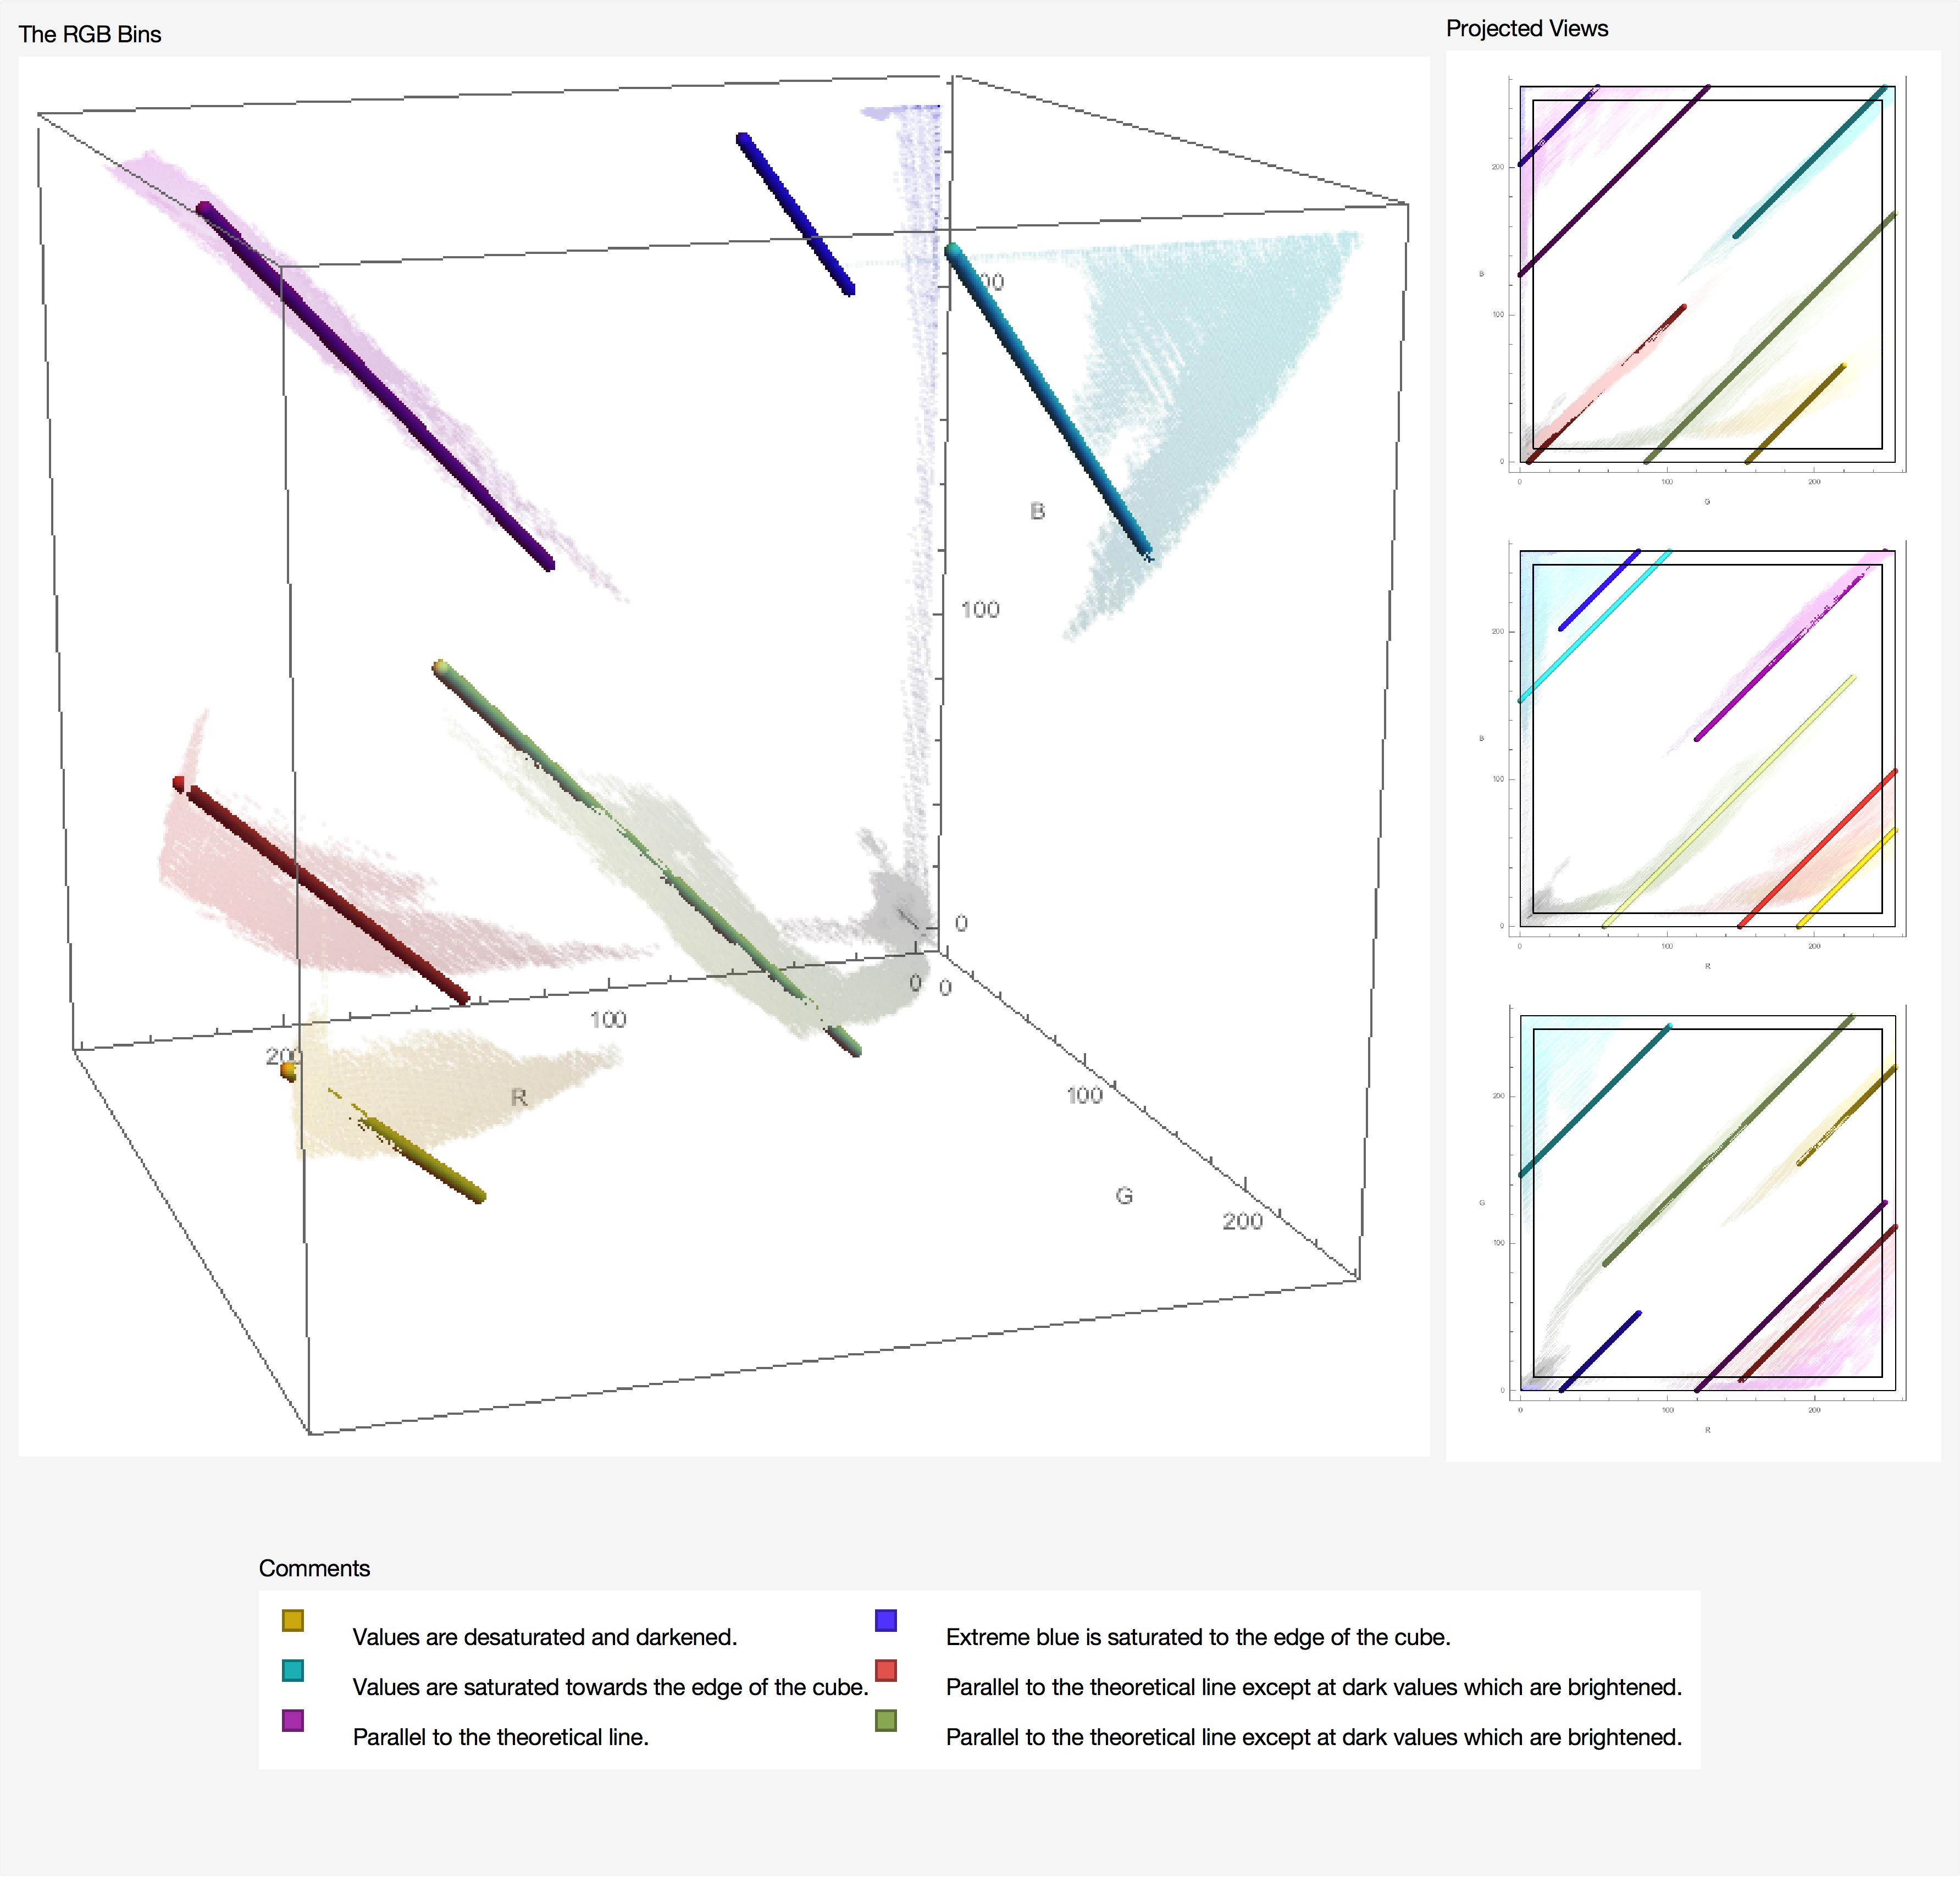
\includegraphics[width=0.98\textwidth]{Chapter3/Figs/Theory_And_Practice.jpg}
    \caption{The Bins for 6 randomly colored blobs varying only in luminosity with lines indicating the source image colors.}  \label{fig:WhitePoint}
\end{figure}

The white point for the iPhone camera was found by taking a random set of 6 colors $X=\left\{ \left\{X^1_R +\lambda, X^1_G  +\lambda, X^1_B +\lambda \right\}, \cdots \right\} $. and varying the luminosity between  $ \lambda(X)_B < \lambda  < \lambda(X)_W$. This produces a set of 6 colors which vary only in luminosity and which do not suffer from white-out or black-out. Panels of these 6 colors with randomly selected luminosity for each were presented to the camera. This produced a set of images and the statistics were collected for this set. Theoretically we expect there to be 6 distinct parallel lines which are also parallel to the line from black to the white point of the camera. If the white point of the camera is not $\left\{ 255,255,255\right\}$ then this test should allow the determination of the real white point. 

The iPhone's white point is always set to the corner of the RGB cube before the image reaches the AP layer. So, when developing an algorithm for the iPhone, white point correction is not necessary, while on other devices the algorithm may need to be adapted accordingly.
\subsection{Color Correction Pre-processing}
A second undocumented pre-processing stage became apparent while gathering skin statistics. The original approach taken used a set of photos of an individual's skin  under different lighting conditions against a constant monochromatic background captured with the iPhone camera. The background was included in order to obtain data on the edges of the skin. A background set of photos captured under the same conditions but without the presence of a hand would then be used to produce a statistical model which would be used to negate bin counts from the individual's skin set which corresponded to background values.

Surprisingly, this approached failed to work; the background was not represented well by the collected background statistics (Figure~\ref{fig:BGFailure}).

\begin{figure}[h!]
  \centering
    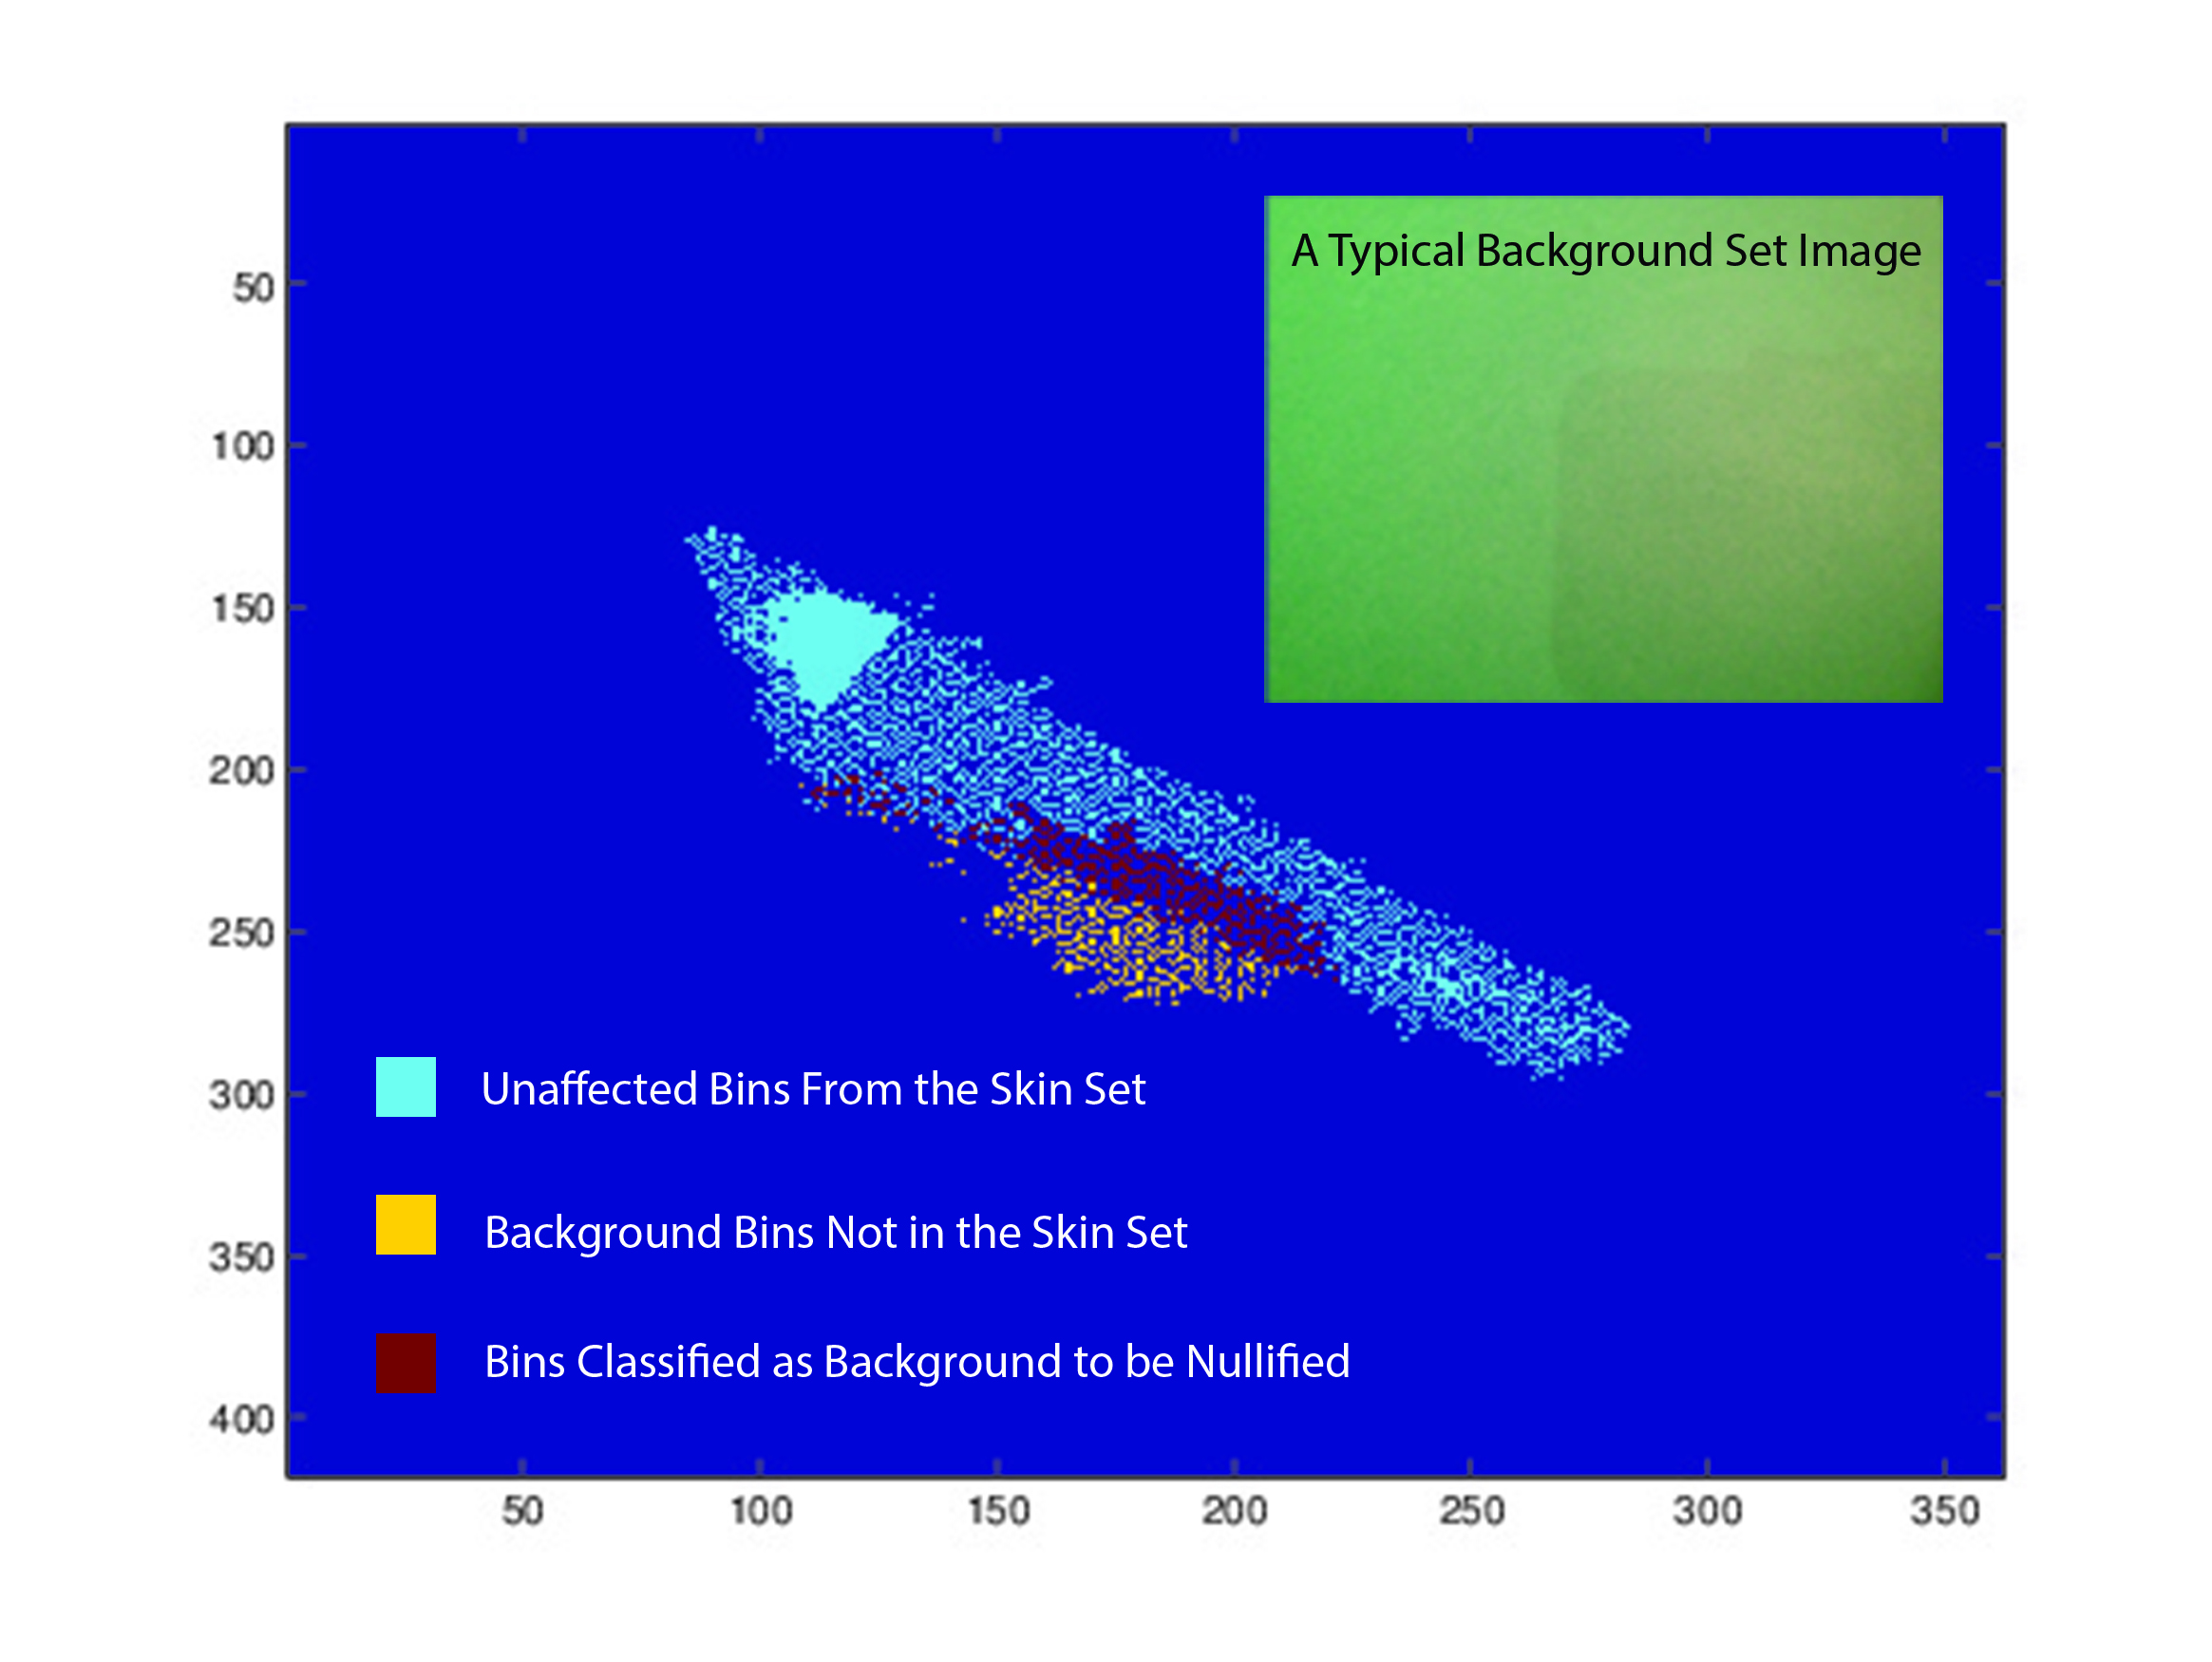
\includegraphics[width=0.95\textwidth]{Chapter3/Figs/CaCb_bg_failed.jpg}
    \caption{Initial attempt at removing background; unsuccessful.} \label{fig:BGFailure}
\end{figure}

The background statistics changed with the skin present in the photo. This is because the iPhone adjusts to images with very strong color characteristics. This color correction is an undocumented feature of the iPhone processing. The only way to compensate for this unwelcome pre-processing is to photograph the background with a strongly contrasting object present, but one which is easily cropped out of the image before the background statistics are collected. After collecting the statistics again, the result was much improved (Figure~\ref{fig:BGSuccess1}).

\begin{figure}[h!]
  \centering
    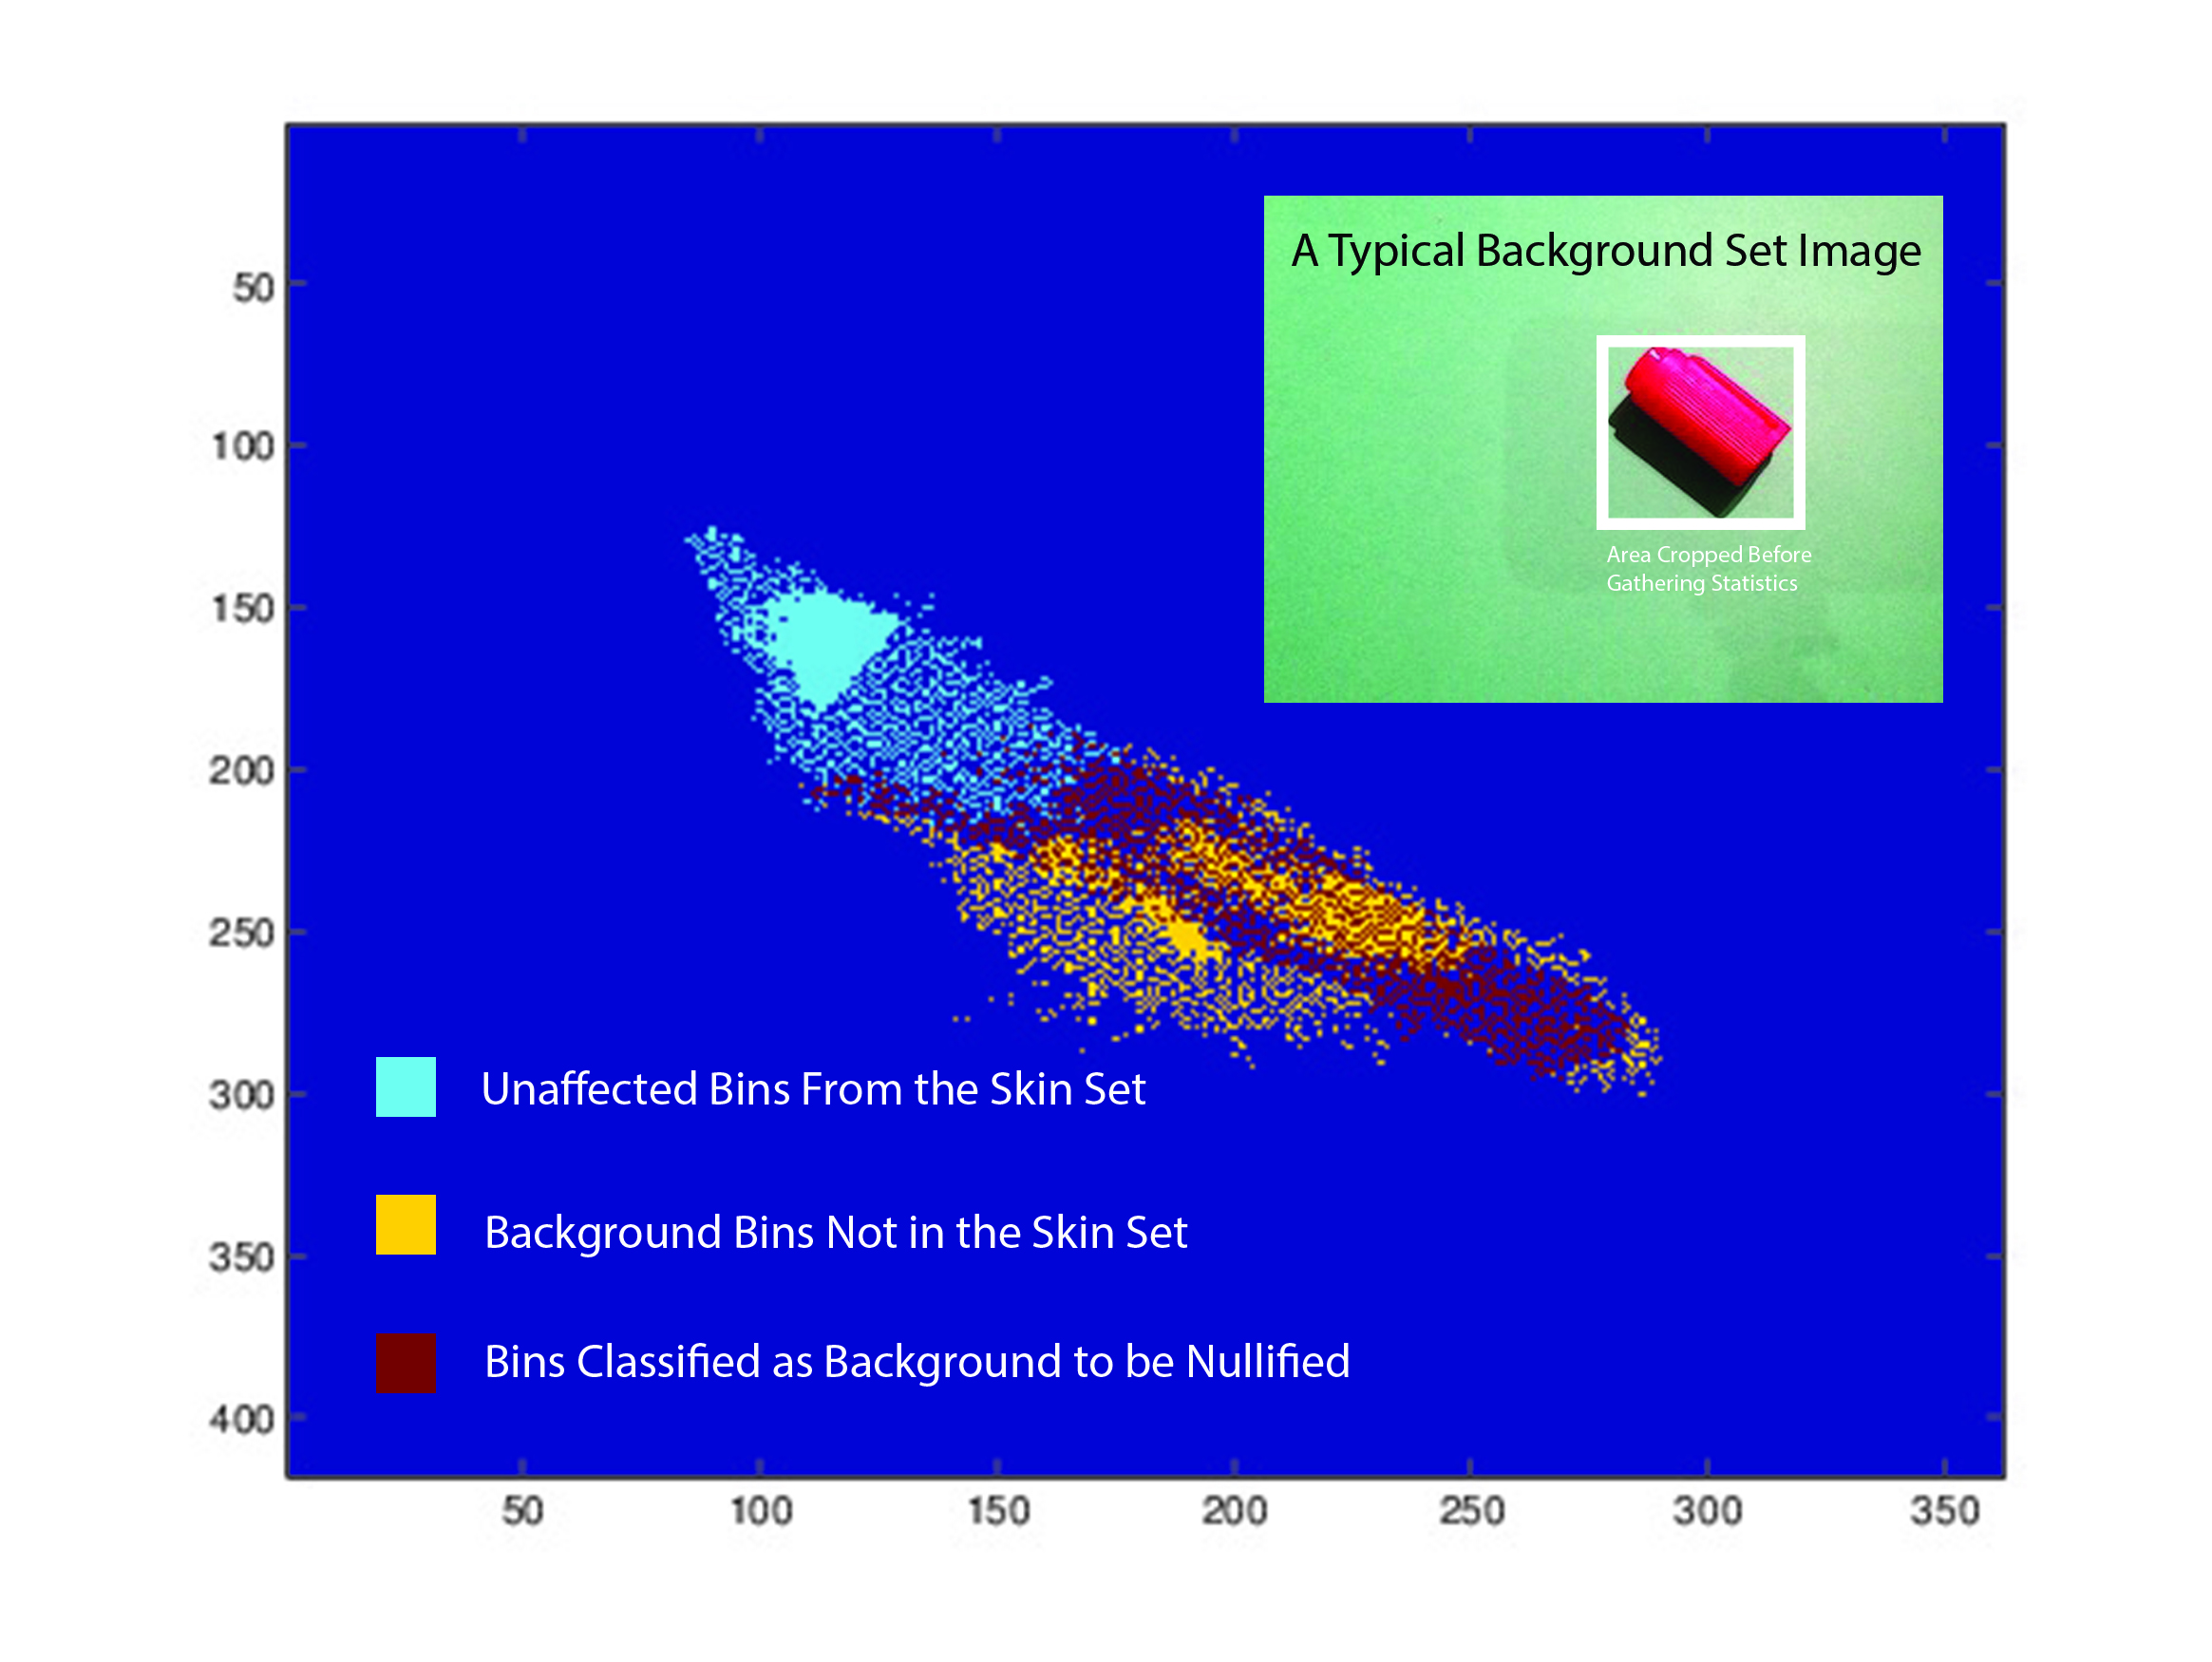
\includegraphics[width=0.80\textwidth]{Chapter3/Figs/CaCb_bg_success.jpg}
    \caption{Successful background removal.}  \label{fig:BGSuccess1}
\end{figure}

In a real world context, it is relatively safe to presume that the scene will be chromatically complex enough that the color correction won't be detrimental to detection, and perhaps even beneficial under unusual lighting conditions. But for gathering statistics, it proved to be a massive pain.

\subsection{White-Out and Black-Out}\label{sec:WhiteoutAndBlackout}
A monochromatic object with average RGB color $\mathbf{\mu}=\left\{\mu_R, \mu_G, \mu_B \right\}$ under different lighting conditions produce an in-camera value of $\left\{\mu_R +\lambda, \mu_G  +\lambda, \mu_B +\lambda \right\}$. Each channel has a numerical limit which means that when that limit is reached further change in luminosity $\lambda$ will result in a change in chromatic value. At high luminosities the colors converge on white becoming washed out. This is referred to as white-out. Similarly at low luminosities the colors converge on black which is referred to as black-out.

\begin{figure}[h!] %hi-res
  \centering
    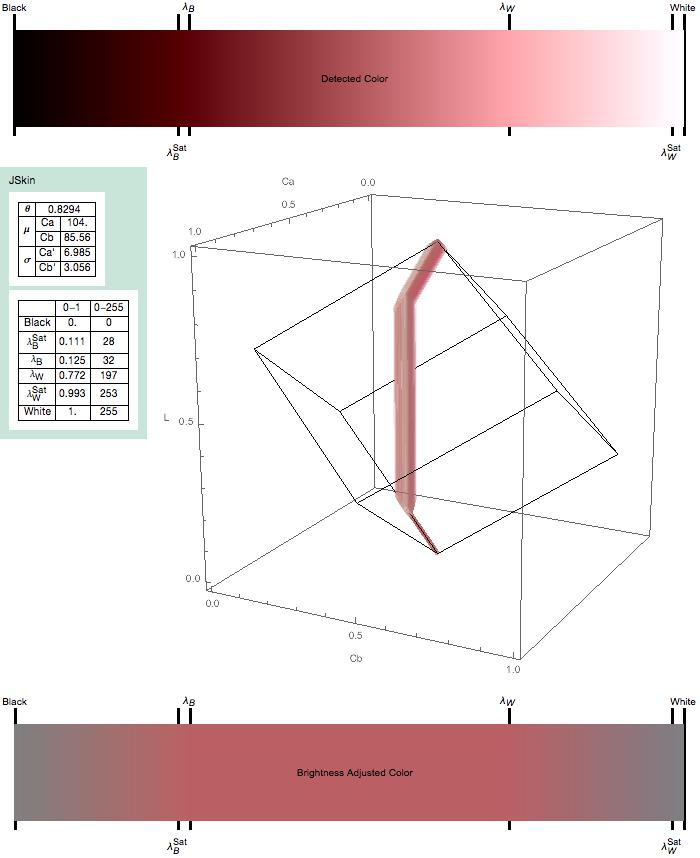
\includegraphics[width=0.80\textwidth]{Chapter3/Figs/WOBOFig.jpg}
    \caption{White-out and Black-out.}  \label{fig:WoBo1}
\end{figure}

It is reasonable to assume that pixel values which contain fully saturated channel elements are unreliable as they may be the result of white-out or black-out. Unfortunately the iPhone also performs an auto brightness and contrast adjustment moving pixel values away from the sides of the RGB cube. The result of this processing is that the values with a luminosity above $\lambda_w$ and below $\lambda_b$ are unreliable.

\section{Algorithm for Generating the Model}\label{sec:AlgorithmForGeneratingModel}
Here we present the algorithm which is used to generate the chromatic model. It's assumed we have RGB image sets for the target with simple, monochromatic backgrounds.

%\animategraphics[loop,autoplay,controls]{12}{Chapter3/Figs/FSkin/RGB_FSkin_Bin_Animation/frame}{0001}{0025}
%\animategraphics[loop,autoplay,controls]{12}{Chapter3/Figs/FSkin/RGB_FSkin_Bin_Skinned_Animation/frame}{0001}{0025}
%\animategraphics[loop,autoplay,controls]{12}{Chapter3/Figs/FSkin/RGB_FSkin_Bin_Skinned_Rot_Animation/frame}{0001}{0025}
%\animategraphics[loop,autoplay,controls]{12}{Chapter3/Figs/FSkin/RGB_FSkin_Bin_Skinned_Rot_TopTail_Animation/frame}{0001}{0025}


%\includemedia[
%  label=cube_test,
%  width=0.7\linewidth,height=0.7\linewidth,
%  addresource=Chapter3/Figs/Animation/RGB_FSkin_Hand_Bin.swf, %two video files
%  transparent,
%  activate=pageopen,
%  flashvars={
%    source=Chapter3/Figs/Animation/RGB_FSkin_Hand_Bin.swf
%   &loop=true
%   &scaleMode=letterbox
%  }
%]{}{Chapter3/Figs/Animation/RGB_FSkin_Hand_Bin.swf}


\subsection{RGB Bin Allocation}\label{sec:RGBBinAllocation}


% Choose an individual for the plots
%\def\individual{FJN}
\def\individual{FSkin}
%\def\individual{JSkin}
%\def\individual{NSkin}


\begin{figure}[h!]
  \centering
    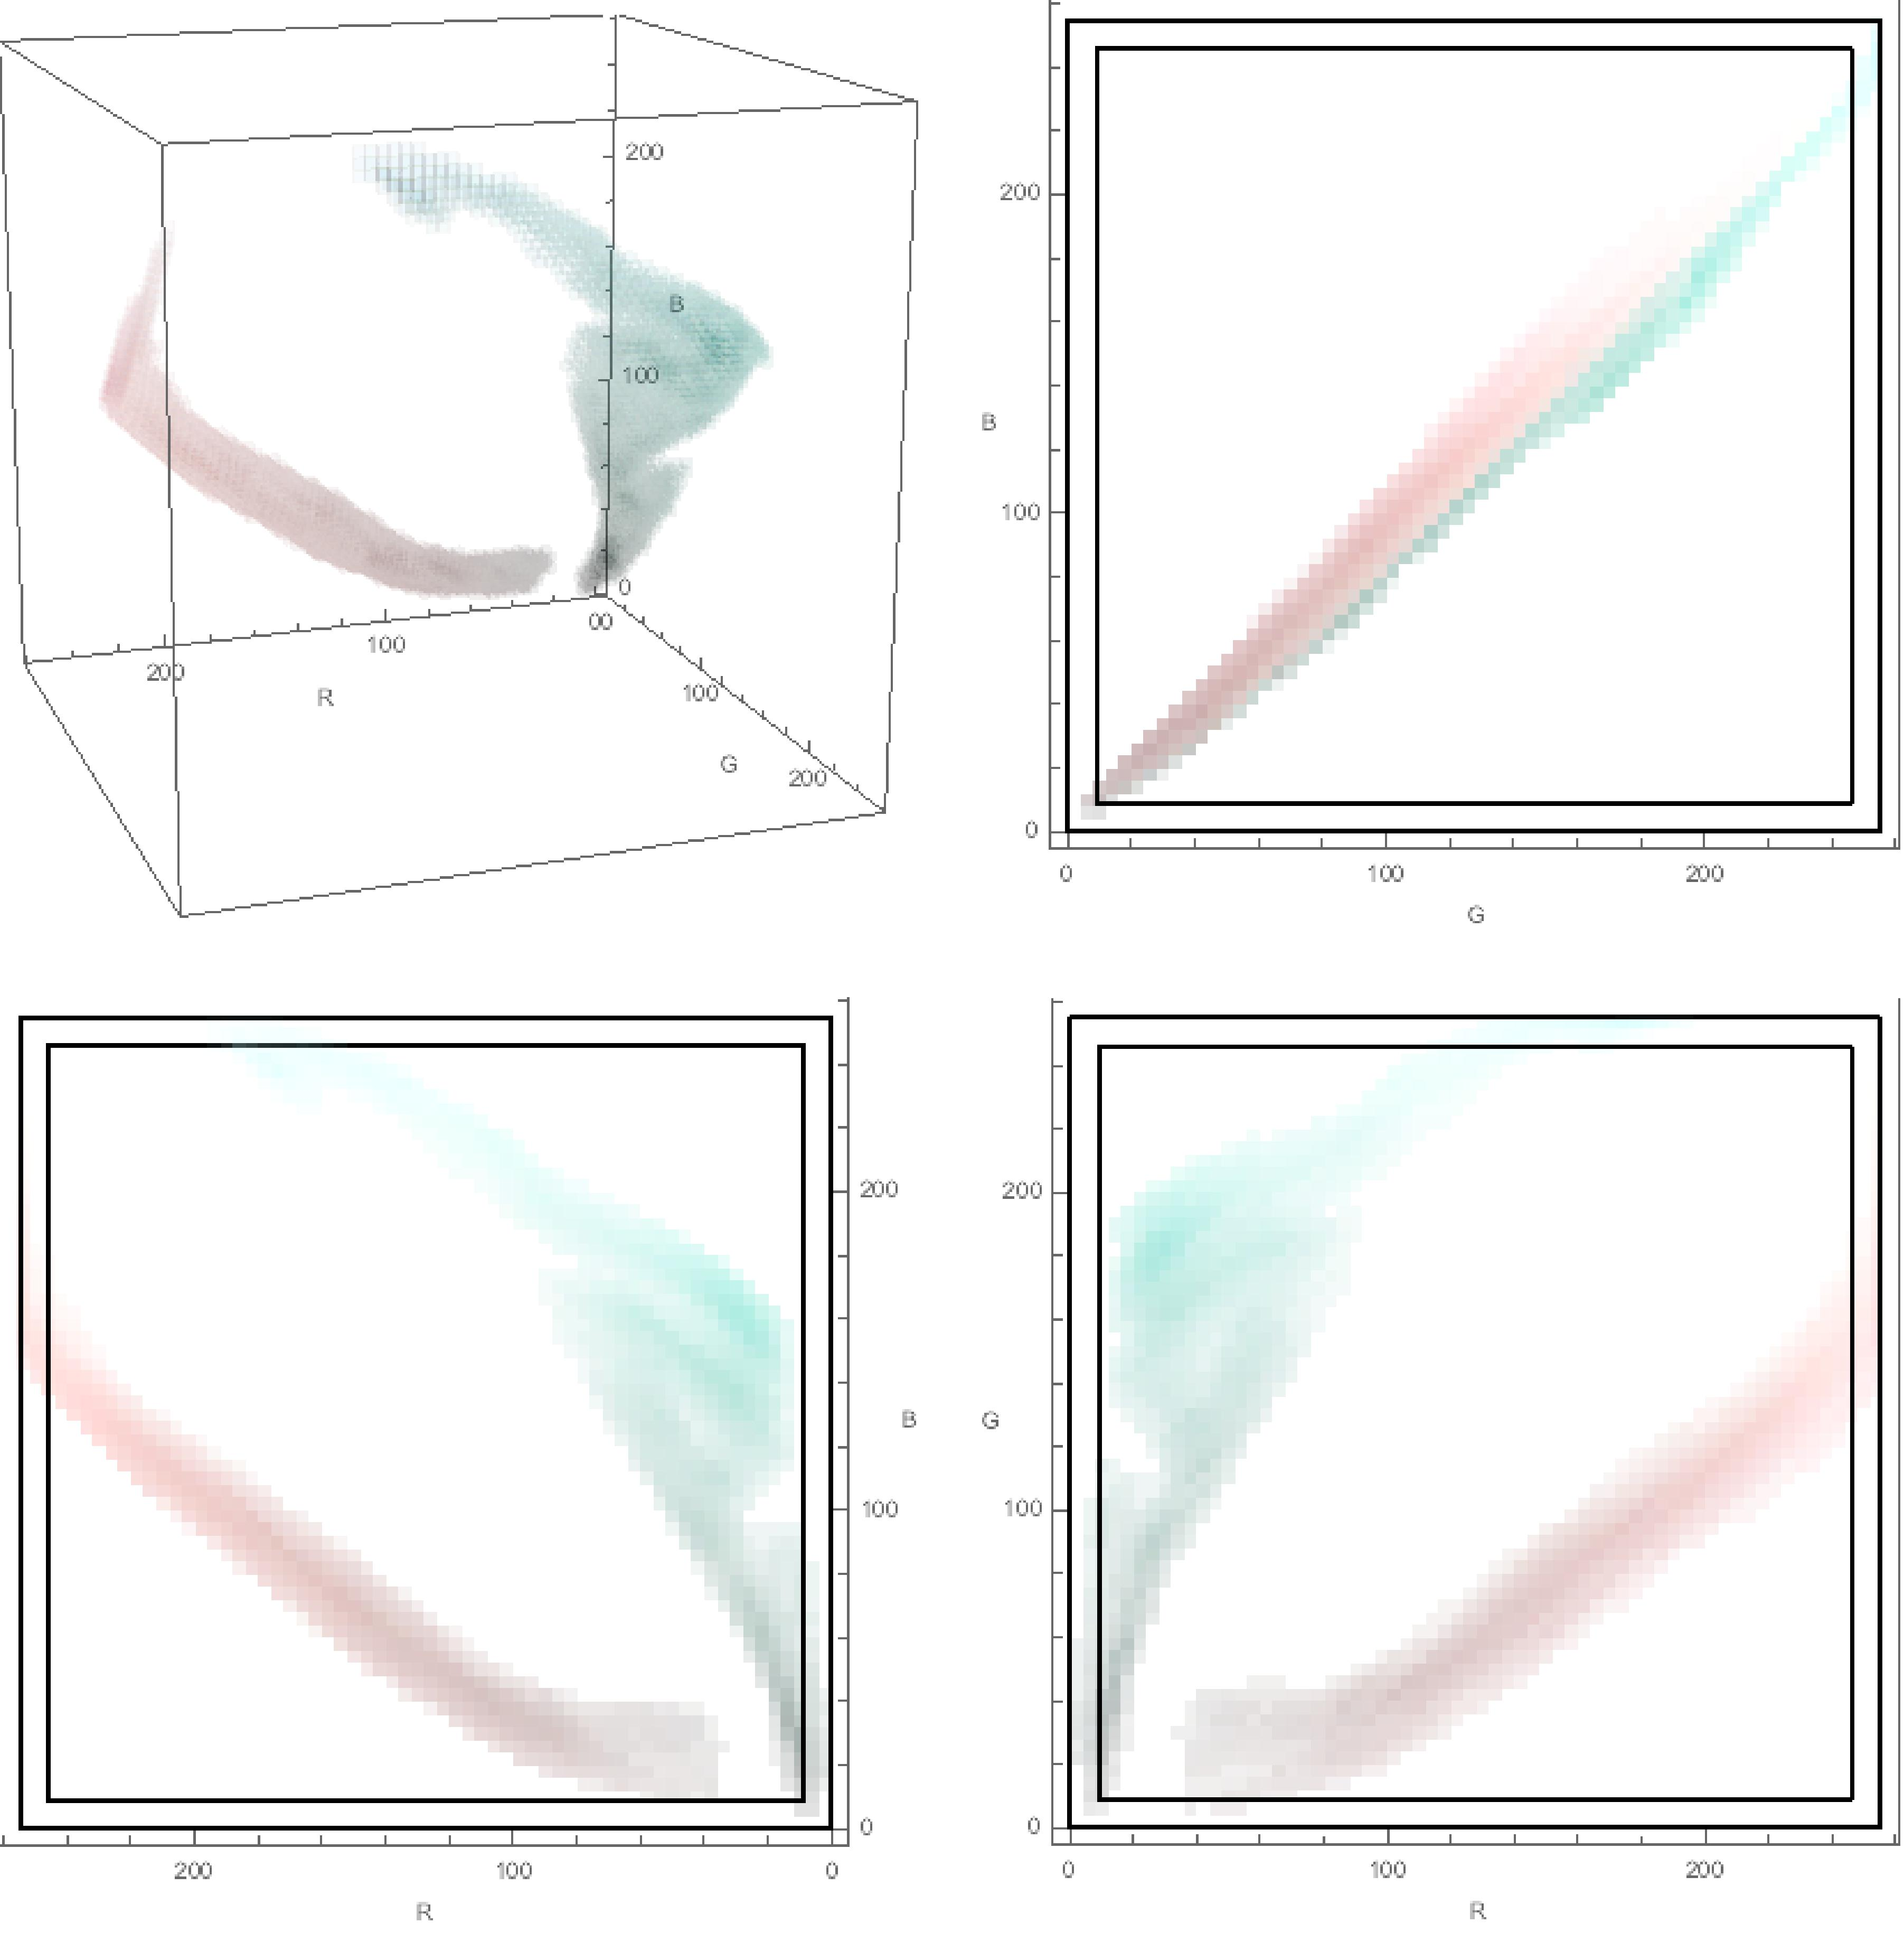
\includegraphics[width=0.9\textwidth]{Chapter3/Figs/\individual/Fill_the_Bins.jpg}
        \caption{\textbf{The 3D RGB histogram}. Distinct distributions can be seen for the Skin and the background. Here the bin color corresponds to the color which that bin represents and the opacity indicates the frequency of that bin value. }  \label{fig:Fill_the_Bins}
    \end{figure}

The first problem is that we have a large image set with large images. We're only interested in the individual pixel values so we produce a 3D histogram with one bin for each RGB combination giving 256x256x256 bins. This is a large data set but it's easier to work with than the set of images and is guaranteed to contain all the relevant information for the statistics.

The histogram bin counting algorithm is written in MATLAB. It runs through each pixel in the image set, proceeding as follows:

\begin{itemize}
\item Increment the corresponding bin.
\item Increment the total pixel count.
\item Is the current bin count larger than the largest bin count so far? If so, increment the largest bin count.
\end{itemize}

So now we have a 3D histogram with a total bin count and a largest bin count.


\subsection{Skinning the Bins}\label{sec:SkinningTheBins}

\begin{figure}[h!] %hi-res
  \centering
    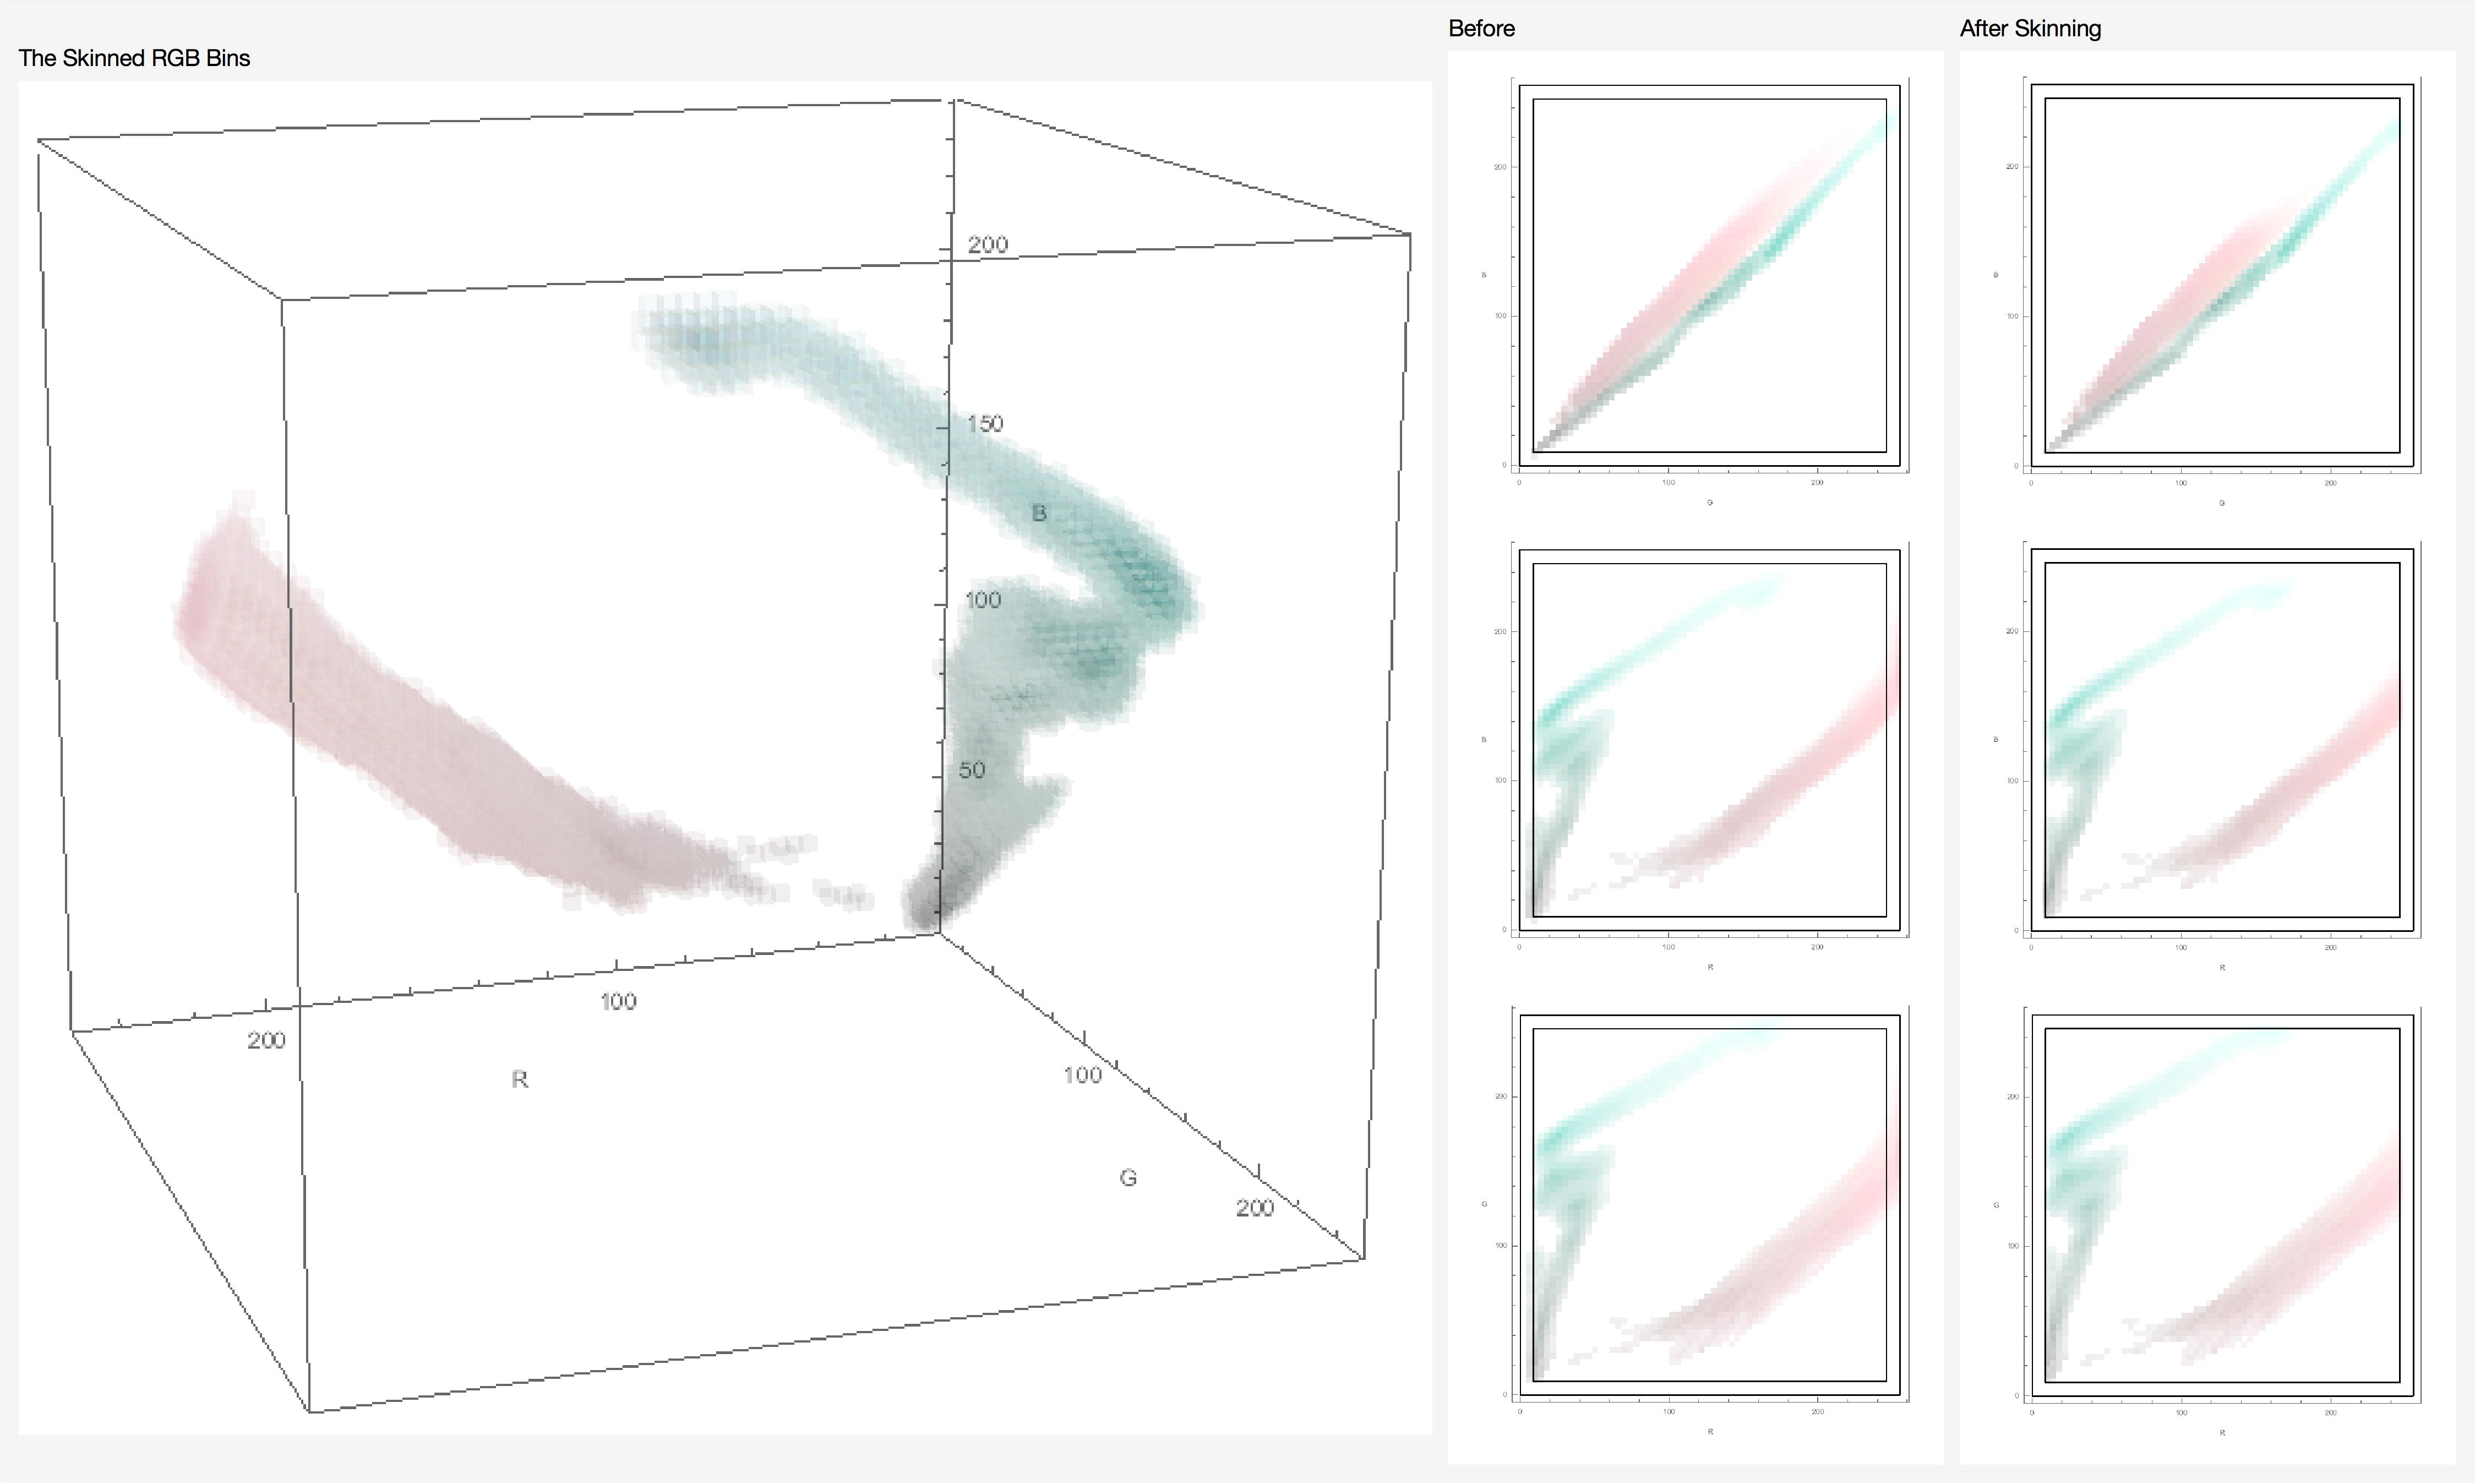
\includegraphics[width=1.0\textwidth]{Chapter3/Figs/\individual/Skin_the_Bins.jpg}
        \caption{\textbf{The 3D RGB histogram after 'skinning'}. Distinct distributions can be seen for the Skin and the background. Here the bin color corresponds to the color which that bin represents and the opacity indicates the frequency of that bin value. Bin counts outside the black lines are set to zero. }  \label{fig:Skin_the_Bins}
    \end{figure}

Next, the bins which are at the extreme edges (i.e. the ones which correspond to the outer faces of the RGB cube) are set equal to 0 with a specified depth. For example: if a depth of 3 is requested, bins of positions 0, 1 and 2, and 253, 254 and 255 are set to 0 in all three dimensions, and the total pixel count is adjusted to compensate for the nulled bin counts. This is done to address problems of white-out and black-out as described in \ref{sec:WhiteoutAndBlackout}.



It should be noted that the reason the RGB cube is skinned before rotation is because it's not as easy to do in the rotated color-space.


\subsection{Rotating the Bins}\label{sec:RotatingTheBins}

\begin{figure}[h!] %hi-res
  \centering
    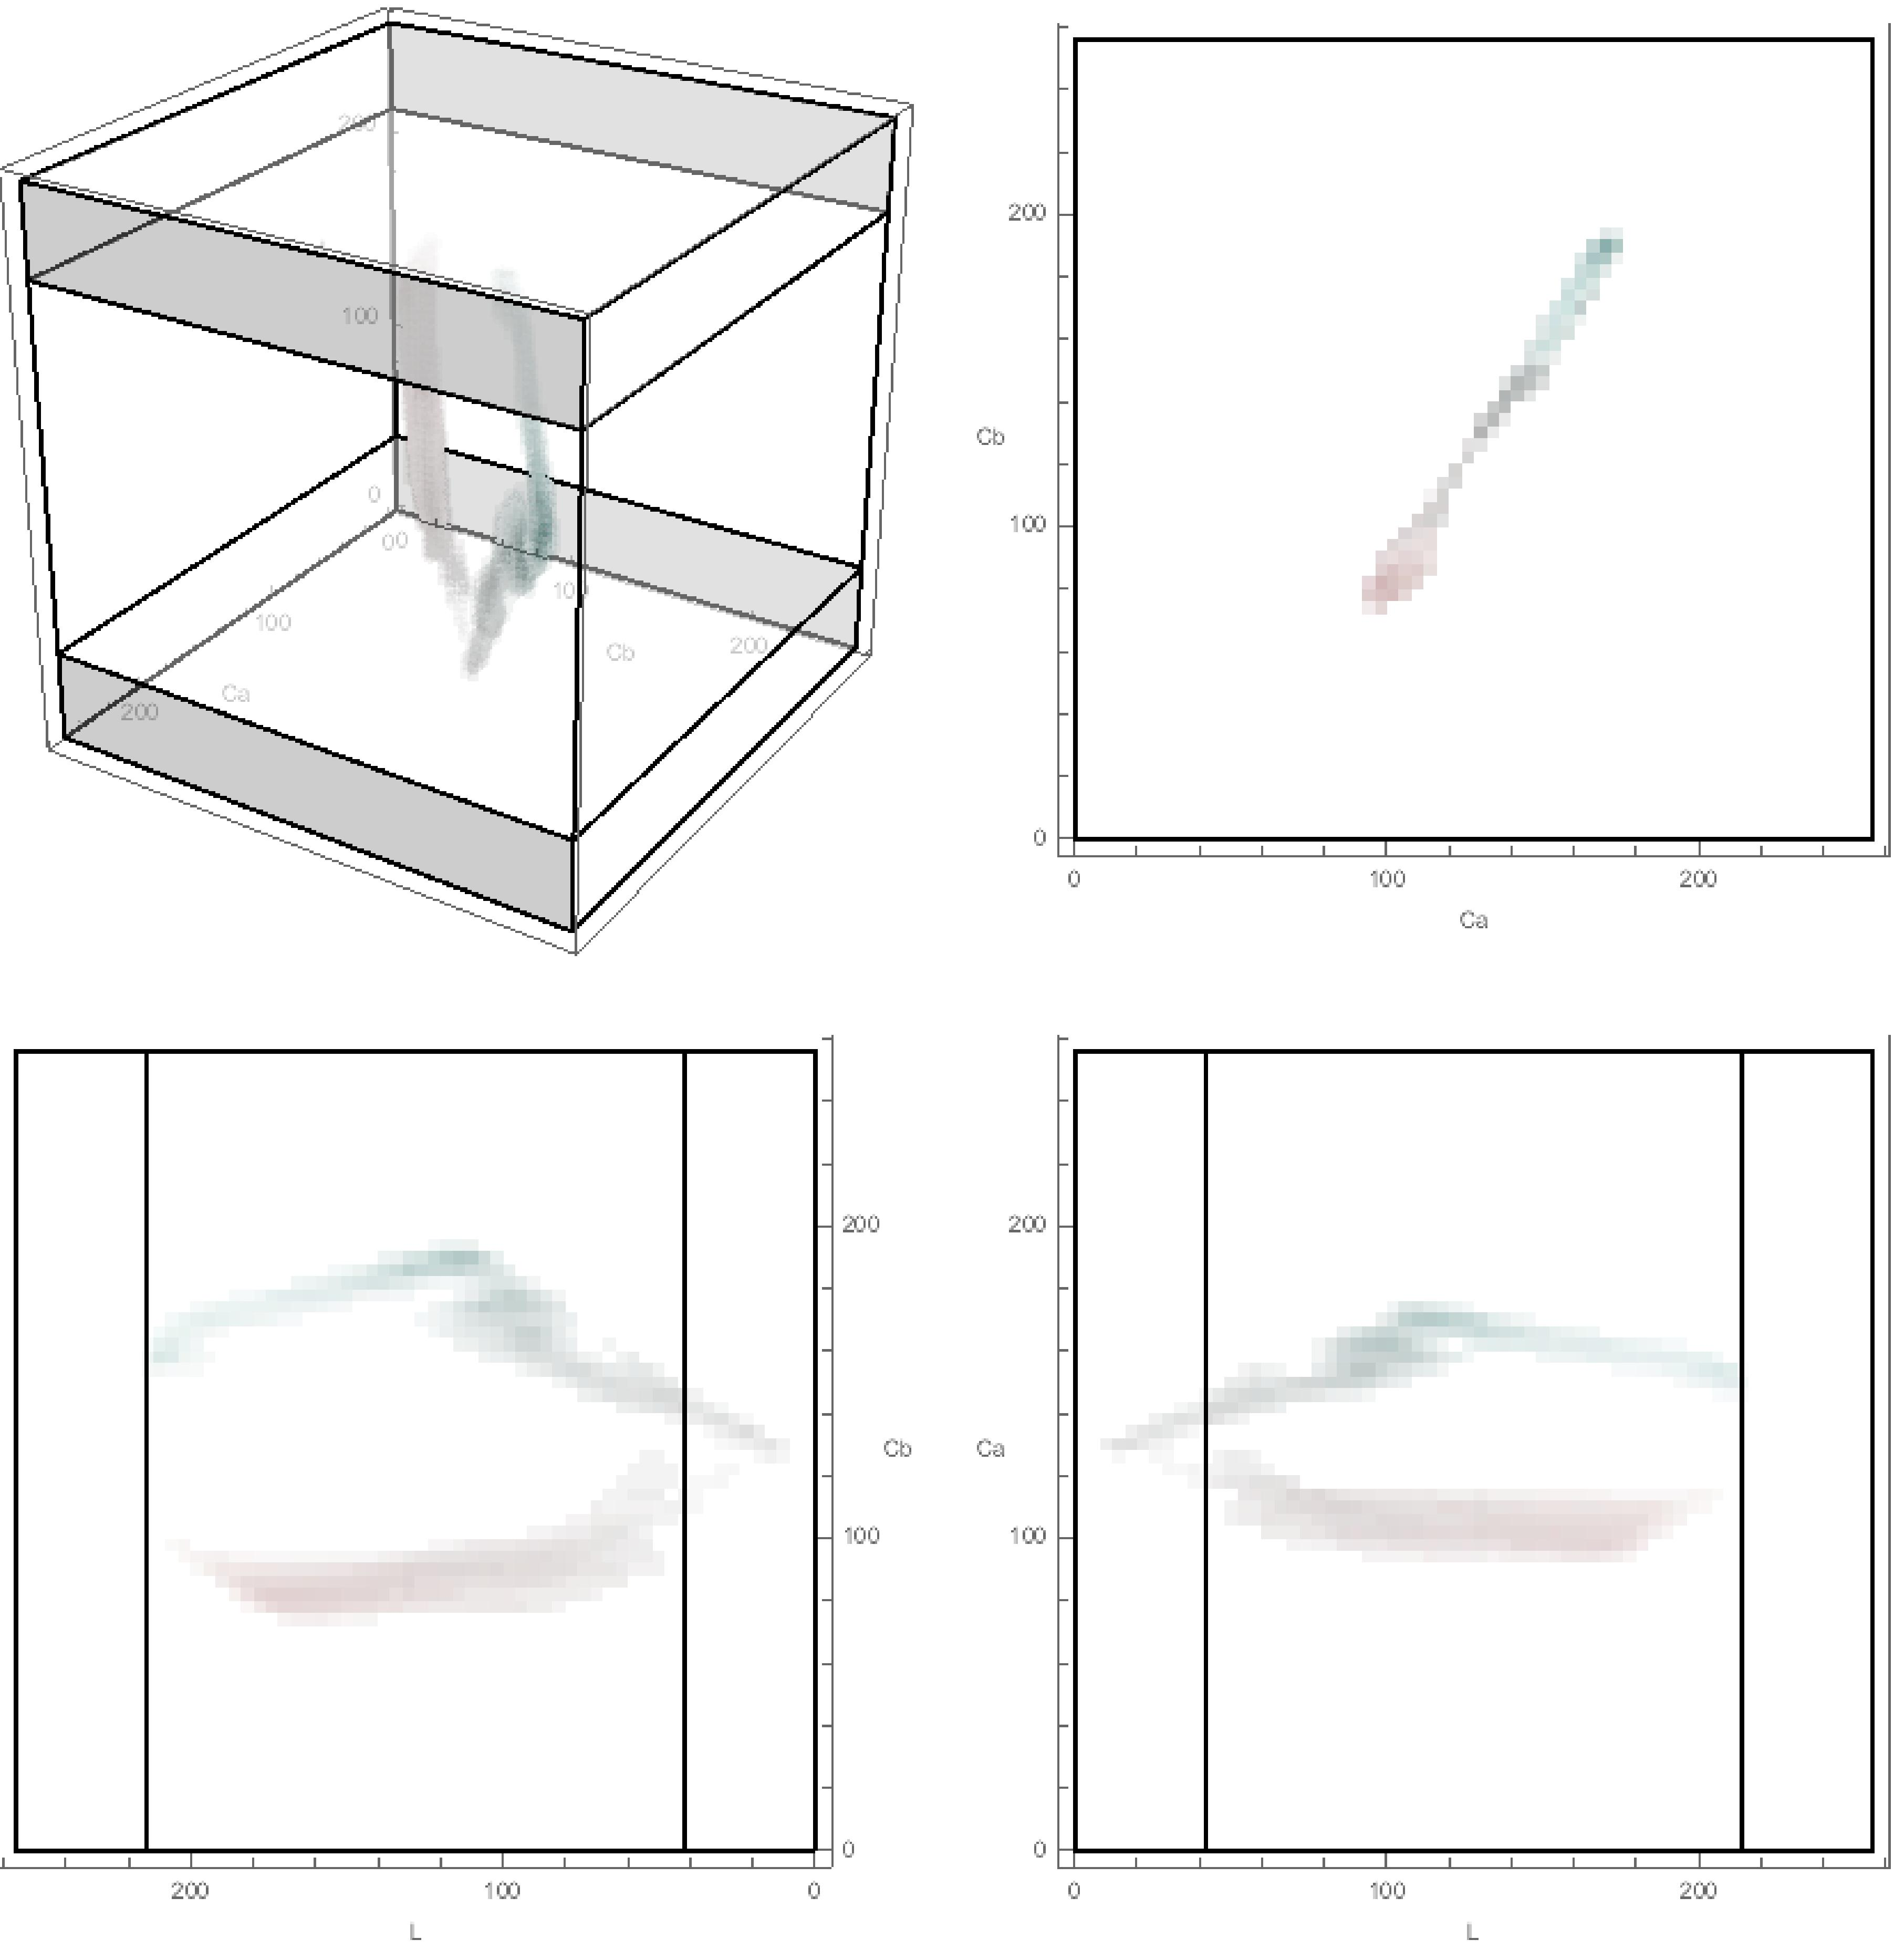
\includegraphics[width=1.0\textwidth]{Chapter3/Figs/\individual/Rotate_the_Bins.jpg}
        \caption{\textbf{The 3D RGB histogram after rotation}. The skin and background distributions can be seen for the Skin and the background. Here the bin color corresponds to the color which that bin represents and the opacity indicates the frequency of that bin value. Bin counts outside the black lines are set to zero. }   \label{fig:Rotate_the_Bins}
\end{figure}

Because each of the bins corresponds to just one RGB value, we can find the equivalent bin in the LCaCb space simply by rotating the bin index. This is done using the normalized rotation as described in Chapter 2. The normalized rotation is used as we desire the mean $\mu$ and standard deviation $\sigma$ to be specified in the $0:1$ range, which is easier to find where all the axes are of the same length. With this done, we now have a set of bins in the LCaCb color-space equivalent to that which would be found if we had applied the transform to each of the images and then collected the statistics from the transformed images.





\subsection{Top and Tail}\label{sec:TopAndTail}

\begin{figure}[h!] %hi-res
  \centering
    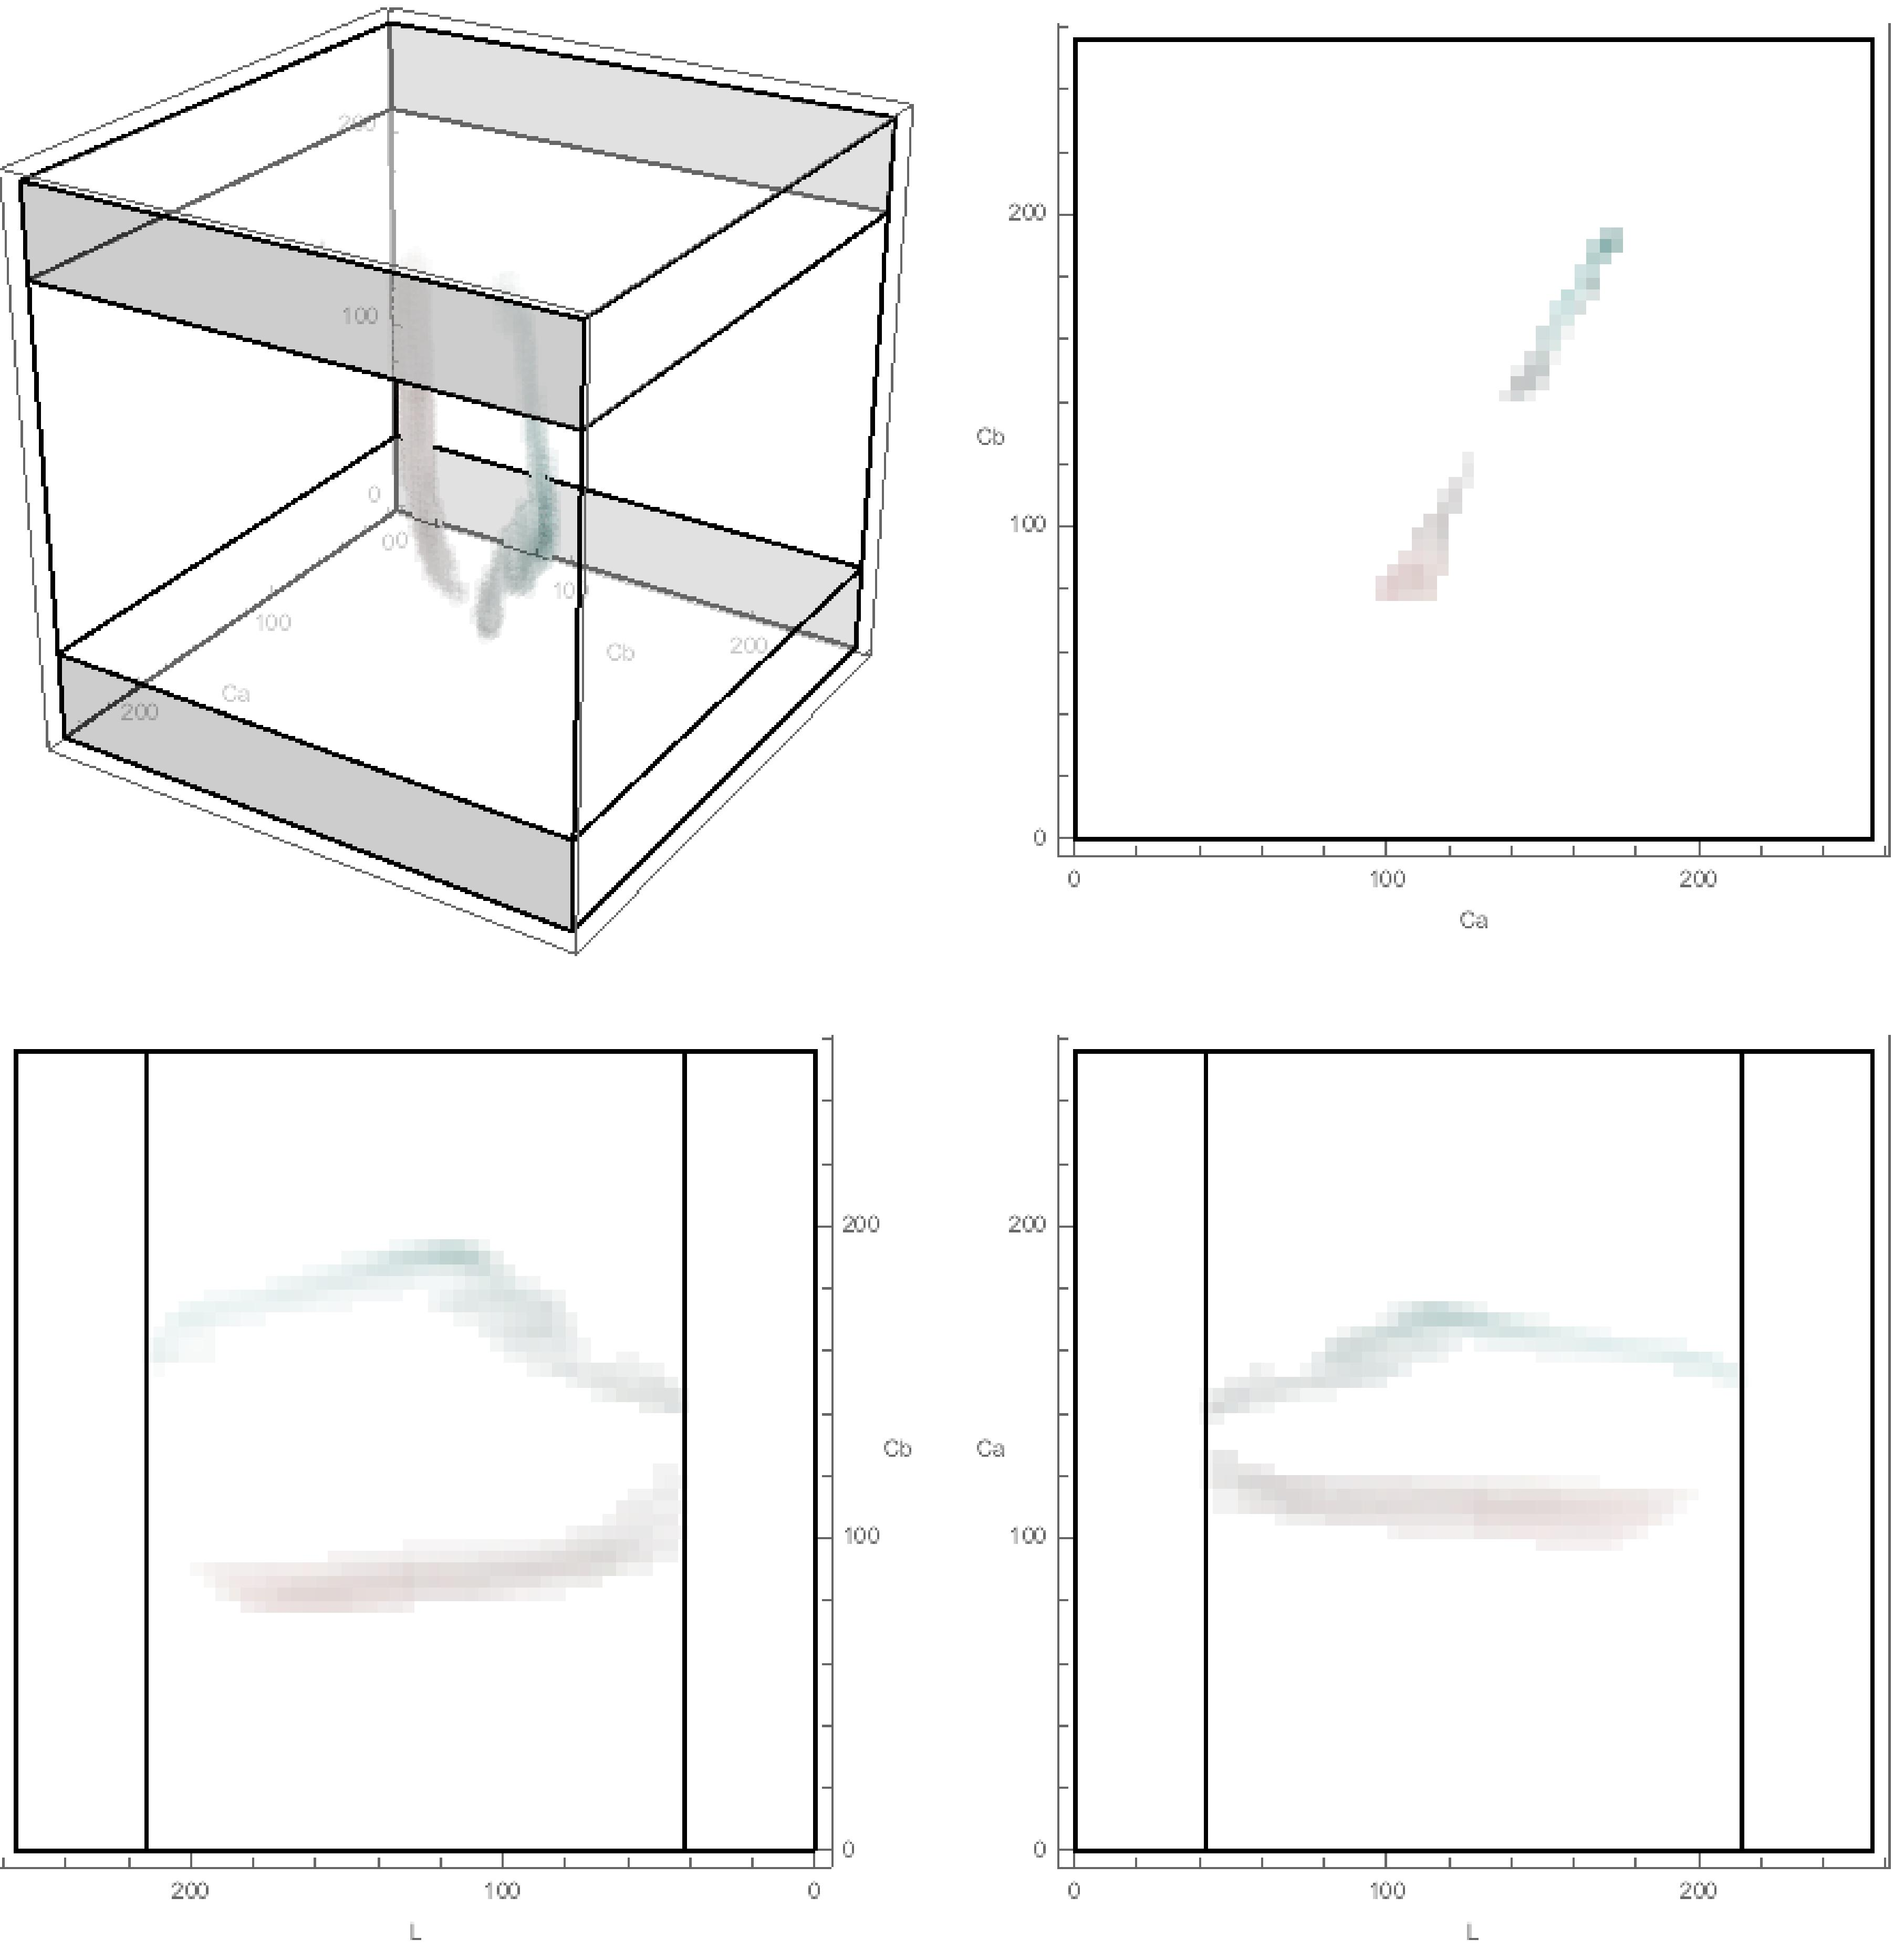
\includegraphics[width=0.9\textwidth]{Chapter3/Figs/\individual/Top_and_Tail_the_Bins.jpg}
        \caption{Filling the RGB Bins}  \label{fig:Top_and_Tail_the_Bins}
    \end{figure}


Naively collapsing the bins along the luminosity axis artificially skews the chromatic distribution along the axis which passed through the luminosity axis; this is easily explained due to white-out and black-out (\ref{sec:WhiteoutAndBlackout}). 
Although we've "skinned" the bins, the white and black tips of the cube suffer from white-out and black-out more than any other regions, and there's a tendency for pixel values to converge under the white point and the black point without necessarily hitting the side of the cube first due to the iPhone contrast and brightness adjustment. This can be seen in Figure   \ref{fig:Top_and_Tail_the_Bins}. 

We collapse the bins excluding the bins which are clearly suffering from white-out and black-out. This could be done mathematically by taking the bin of the distribution which is furthest from the luminosity axis, and then finding the intersection with the RGB cube when this chromatic value is at its limits, just before it reaches the edge of the cube where it suffers from white-out or black-out. But it's a simple matter to look at the three projections of the 3D LCaCb bins and manually determine the limits for the valid region.


\subsection{Collapsing the Bins}\label{sec:CollapsingTheBins}

\begin{figure}[h!]
  \centering
    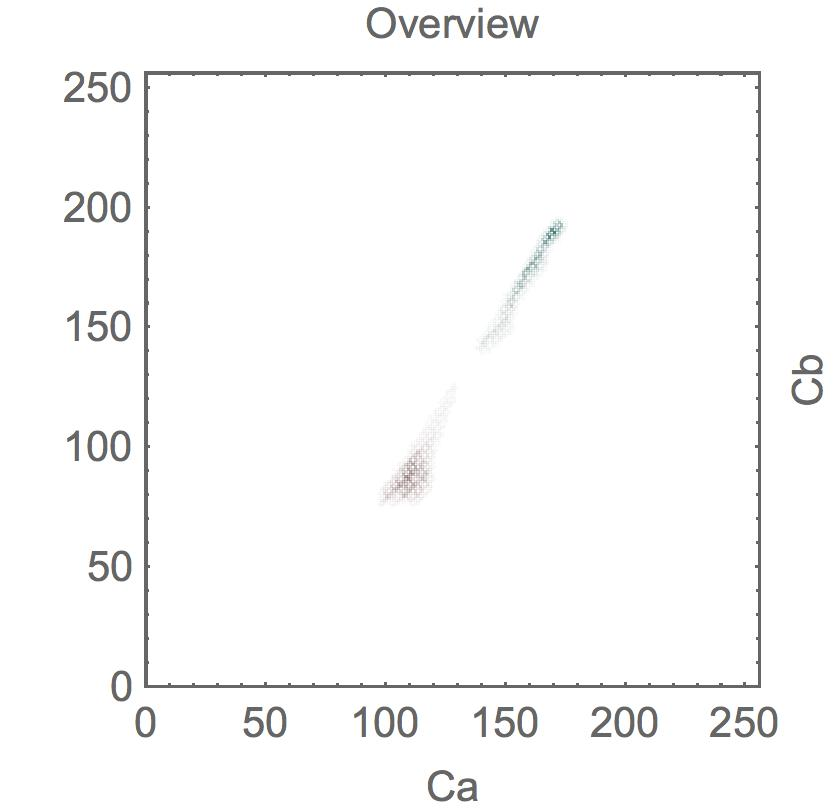
\includegraphics[width=0.6\textwidth]{Chapter3/Figs/\individual/Collapse_the_Bins.jpg}
        \caption{\textbf{The 2D histogram after summing along the luminosity axis}. The color corresponds to the chromatic value of the bin at average luminosity. The opacity corresponds to the frequency of the chromatic value. }  \label{fig:Collapse_the_Bins}
    \end{figure}
    
Because we're modelling the chromatic space and not the luminosity, we now collapse the 3D histogram by summing the bin values along the luminosity axis. So, we now have a 2D histogram in CaCb chromatic space.





\subsection{De-Speckling the Bin Values}\label{sec:DeSpeckle}

\begin{figure}[h!]
  \centering
    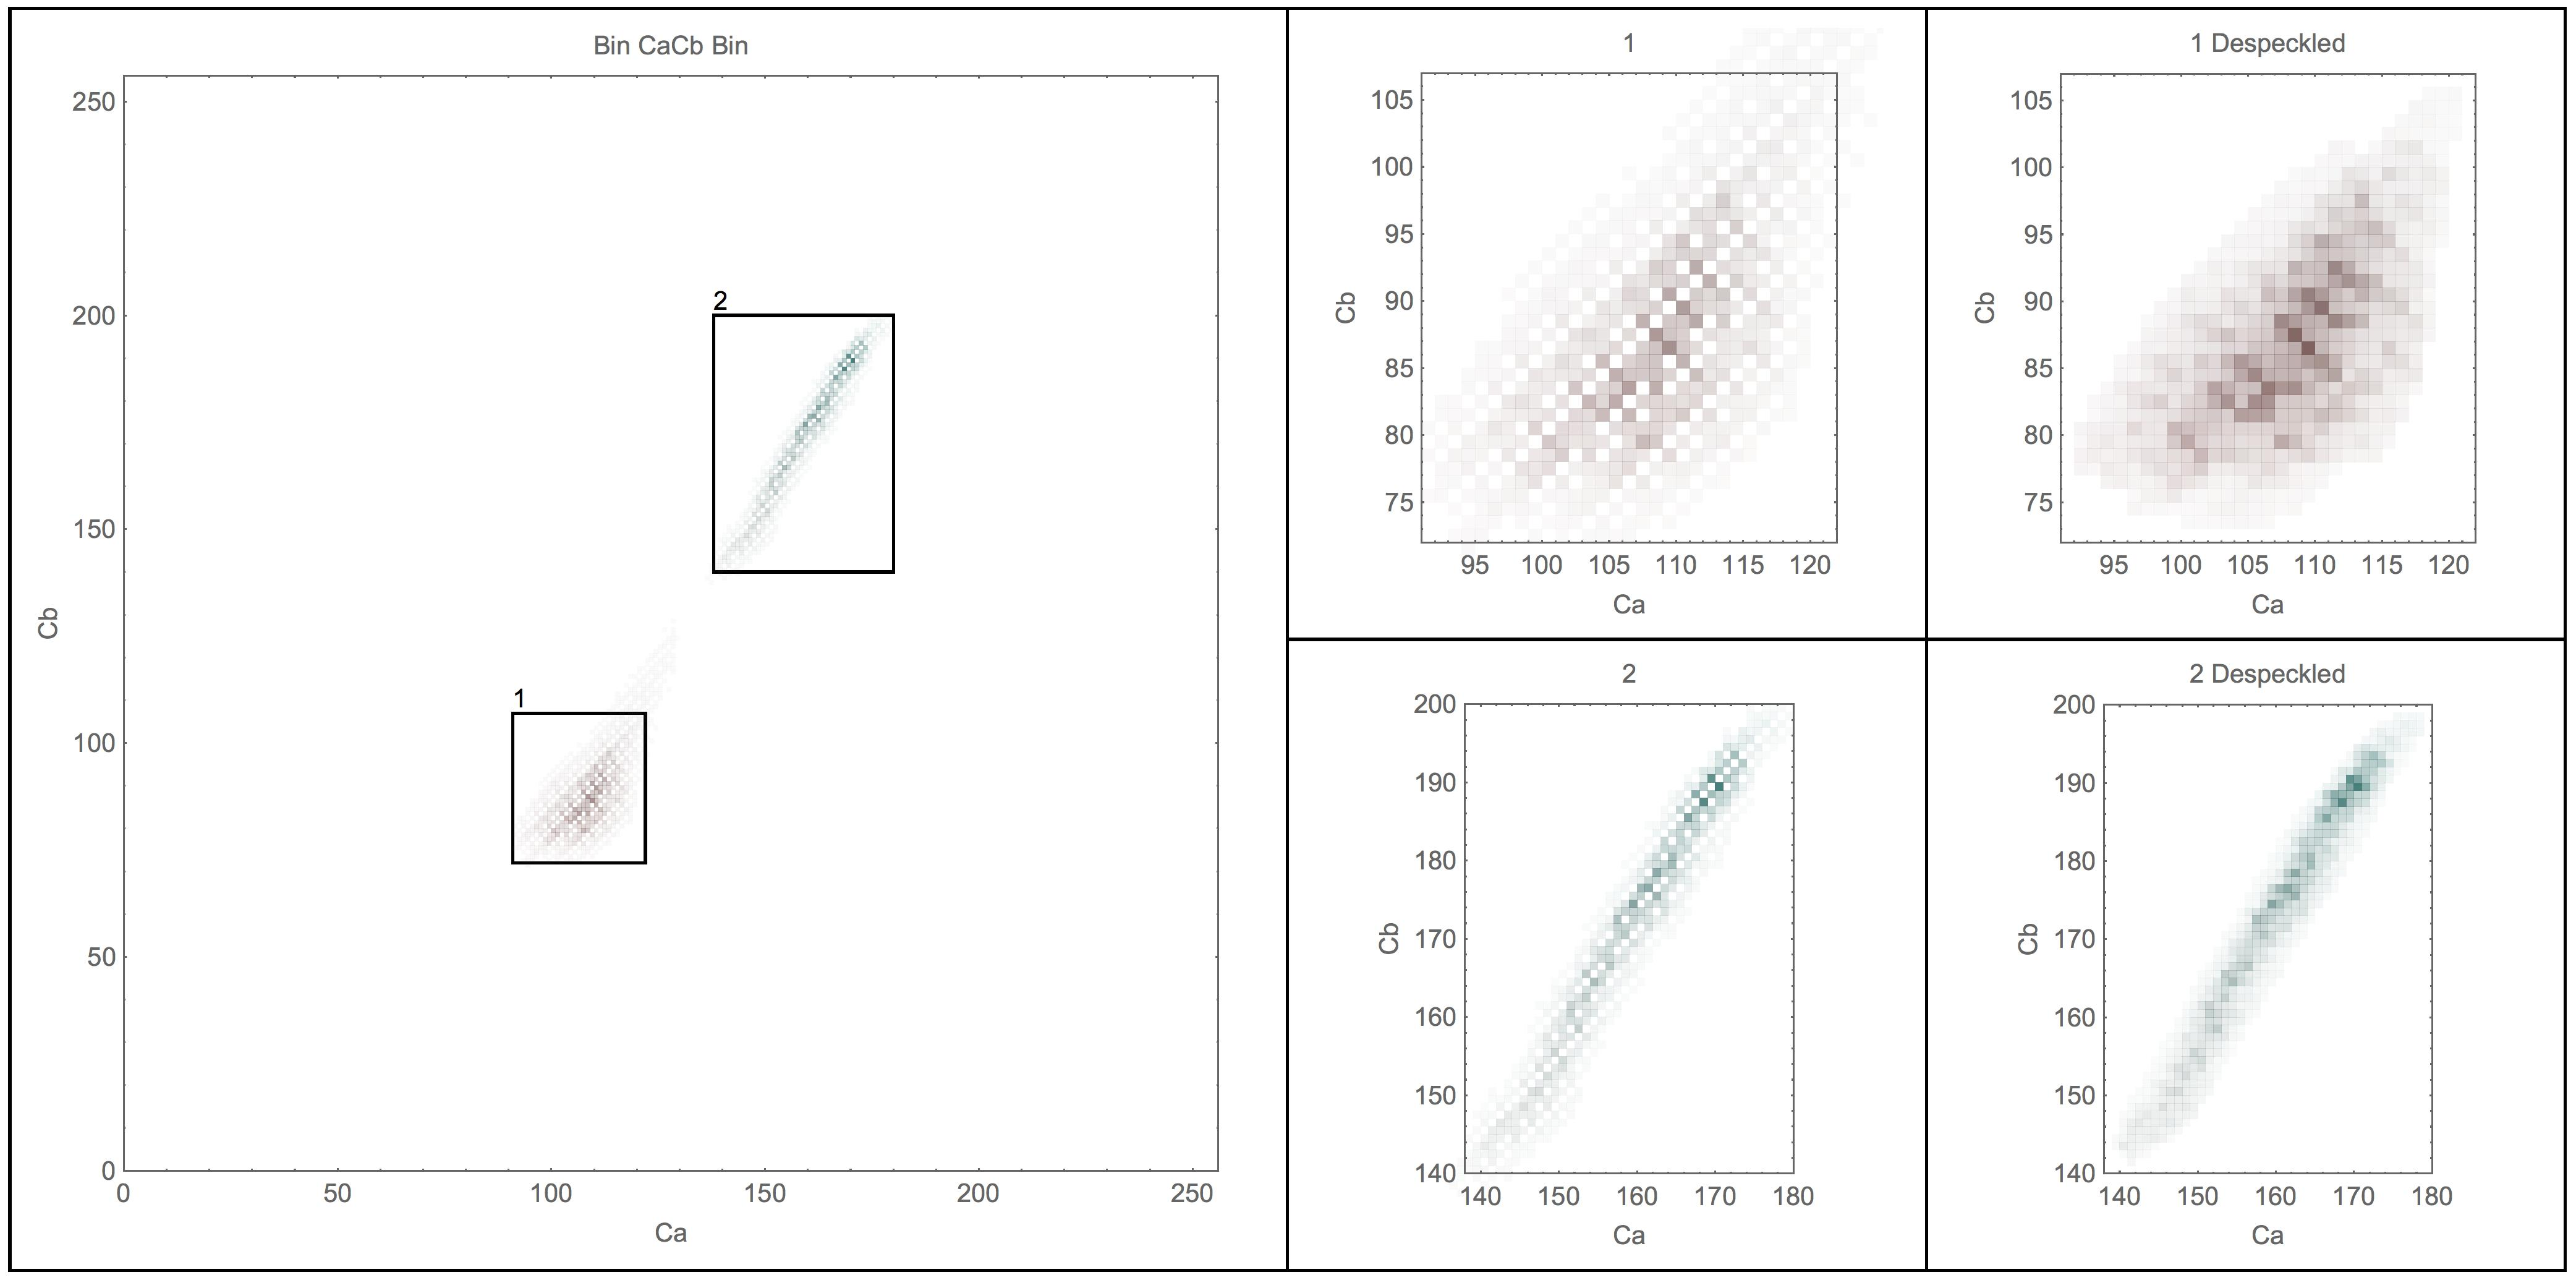
\includegraphics[width=1.0\textwidth]{Chapter3/Figs/\individual/Despeckle_the_Bins.jpg}
        \caption{\textbf{The De-speckled Bins}. The action of the de-speckling algorithm can be seen in the right-hand close-up panels}  \label{fig:Despeckle_the_Bins}
    \end{figure}
    
The raw camera output has, by this stage, undergone two rounds of processing --- first in the device, before the AP layer, creating an 8-bit RGB image; and then in the rotation to the LCaCb space. These processes are, unfortunately, not $1\rightarrow 1$. This results in some bins being artificially overpopulated and other bins becoming artificially empty. The effect of the LCaCb rotation can be controlled by extending the axis lengths; this process can make for at worst $1\rightarrow 1$ correspondence. However, this necessarily introduces a greater number of inaccessible bins. In terms of collecting the statistics, these effects are not problematic aside from the fact that it introduces empty bins inside the main region of interest, which causes difficulties for the algorithm further down the line. Graphically, this problem looks like speckling. This speckling is also apparent in the RGB bins, and so is a result of the pre-processing of the image by the device before the AP layer. It is noteworthy that although the camera claims to capture full 3-channel, 8-bit RGB information, this is not quite true. 

In attempting to solve this problem, the obvious idea is to find all the non-zero bins and fit an interpolating function between them. This will effectively remove the empty bin artefacts within the densely-packed region which is the distribution we're interested in. However, the empty bins outside the main distribution are not artefacts and are genuinely empty bins, so removing all the empty bins and then fitting the function joins together any outlying points or secondary distributions corresponding to regions such as the background. We therefore desire a method which will allow us to keep all the non-empty bins and the empty bins outside the main distribution, i.e. all the genuinely empty bins. To achieve this, we designed a MATLAB routine which essentially paints a region around each non-zero point, marking it as part of the main distribution. It then takes all the unmarked regions and includes all the empty bins in those regions. So, the set of points which is all the non-empty bins and all the empty bins in the unmarked regions satisfies the requirement, and a simple interpolating function can easily be fitted to those points.





\subsection{Blob Detection}\label{sec:BlobDetection}

\begin{figure}[h!]
  \centering
    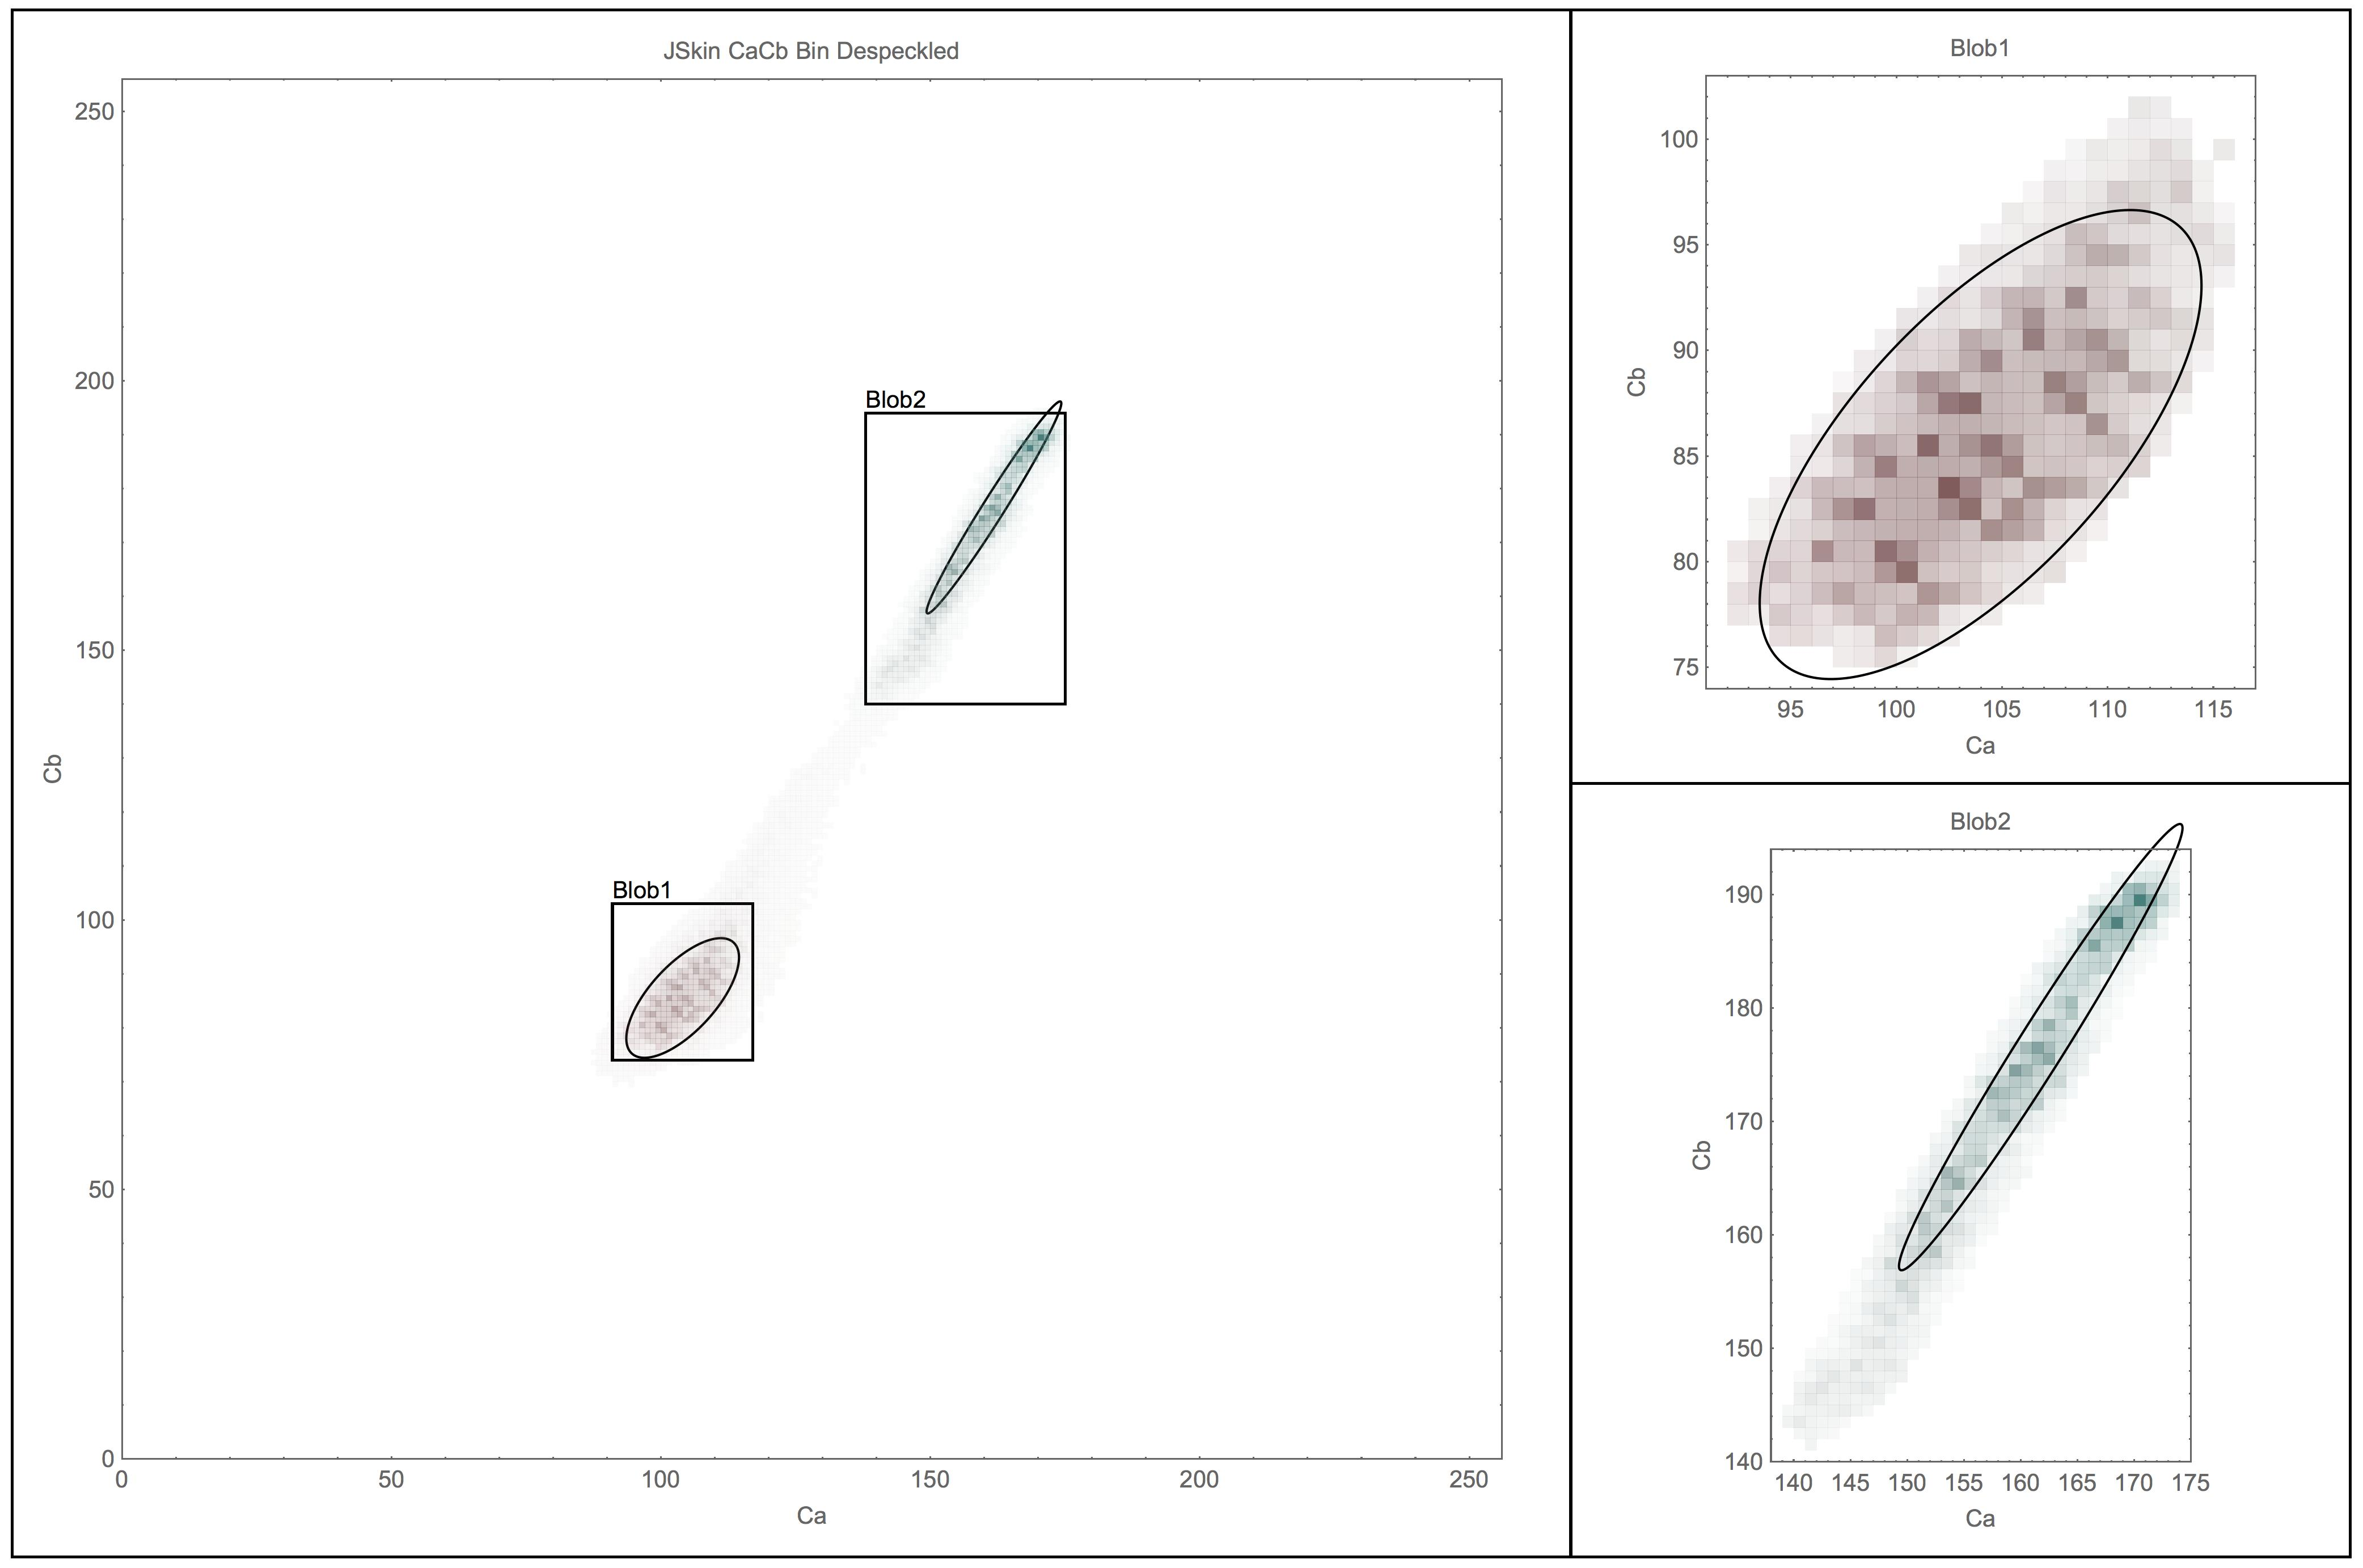
\includegraphics[width=1.0\textwidth]{Chapter3/Figs/\individual/Find_the_Blobs.jpg}
        \caption{\textbf{The Blob Detection.} The detected blobs can be seen in the right-hand panel with the ellipse fit overlayed. The split does not depend on the ellipse but on the extreme edges of the blob.} \label{fig:Find_the_Blobs}
    \end{figure}
    
Having removed the empty bin artefacts and compensated for white-out/black-out effects, the final step is to remove the bin counts of the bins which are associated with the background, thereby leaving a distribution which corresponds to chromatic skin values and which is artefact and systematic-error-free. With the chromatic bins processed as they have been so far, it is clear that there is a distinct distribution for the skin and a distinct distribution for the background.

Using MATLAB's blob detection algorithm, we can find the distinct patches of chromatic information. We expect there to be two distinct blobs: one corresponding to the target skin values, and one to the monochromatic background. The distribution is divided into two, one for each of the detected blobs (Figure \ref{fig:Find_the_Blobs}). The blob detection algorithm also returns the center $\widetilde{\mu}$, eccentricity $\widetilde{\theta}$ and major and minor axis $\widetilde{\sigma}$ for an ellipse which most closely fits the blob shape. The distribution which contains the blob center closest to a reference skin value is chosen to be the skin distribution and the ellipse values are passed to the next step where the Gaussian fit is obtained. Only the bin values between the extreme edges of the blob are passed on to the next stage.

\subsection{The Gaussian Fit}\label{sec:TheGaussianFit}

\begin{figure}[h!] %hi-res
  \centering
    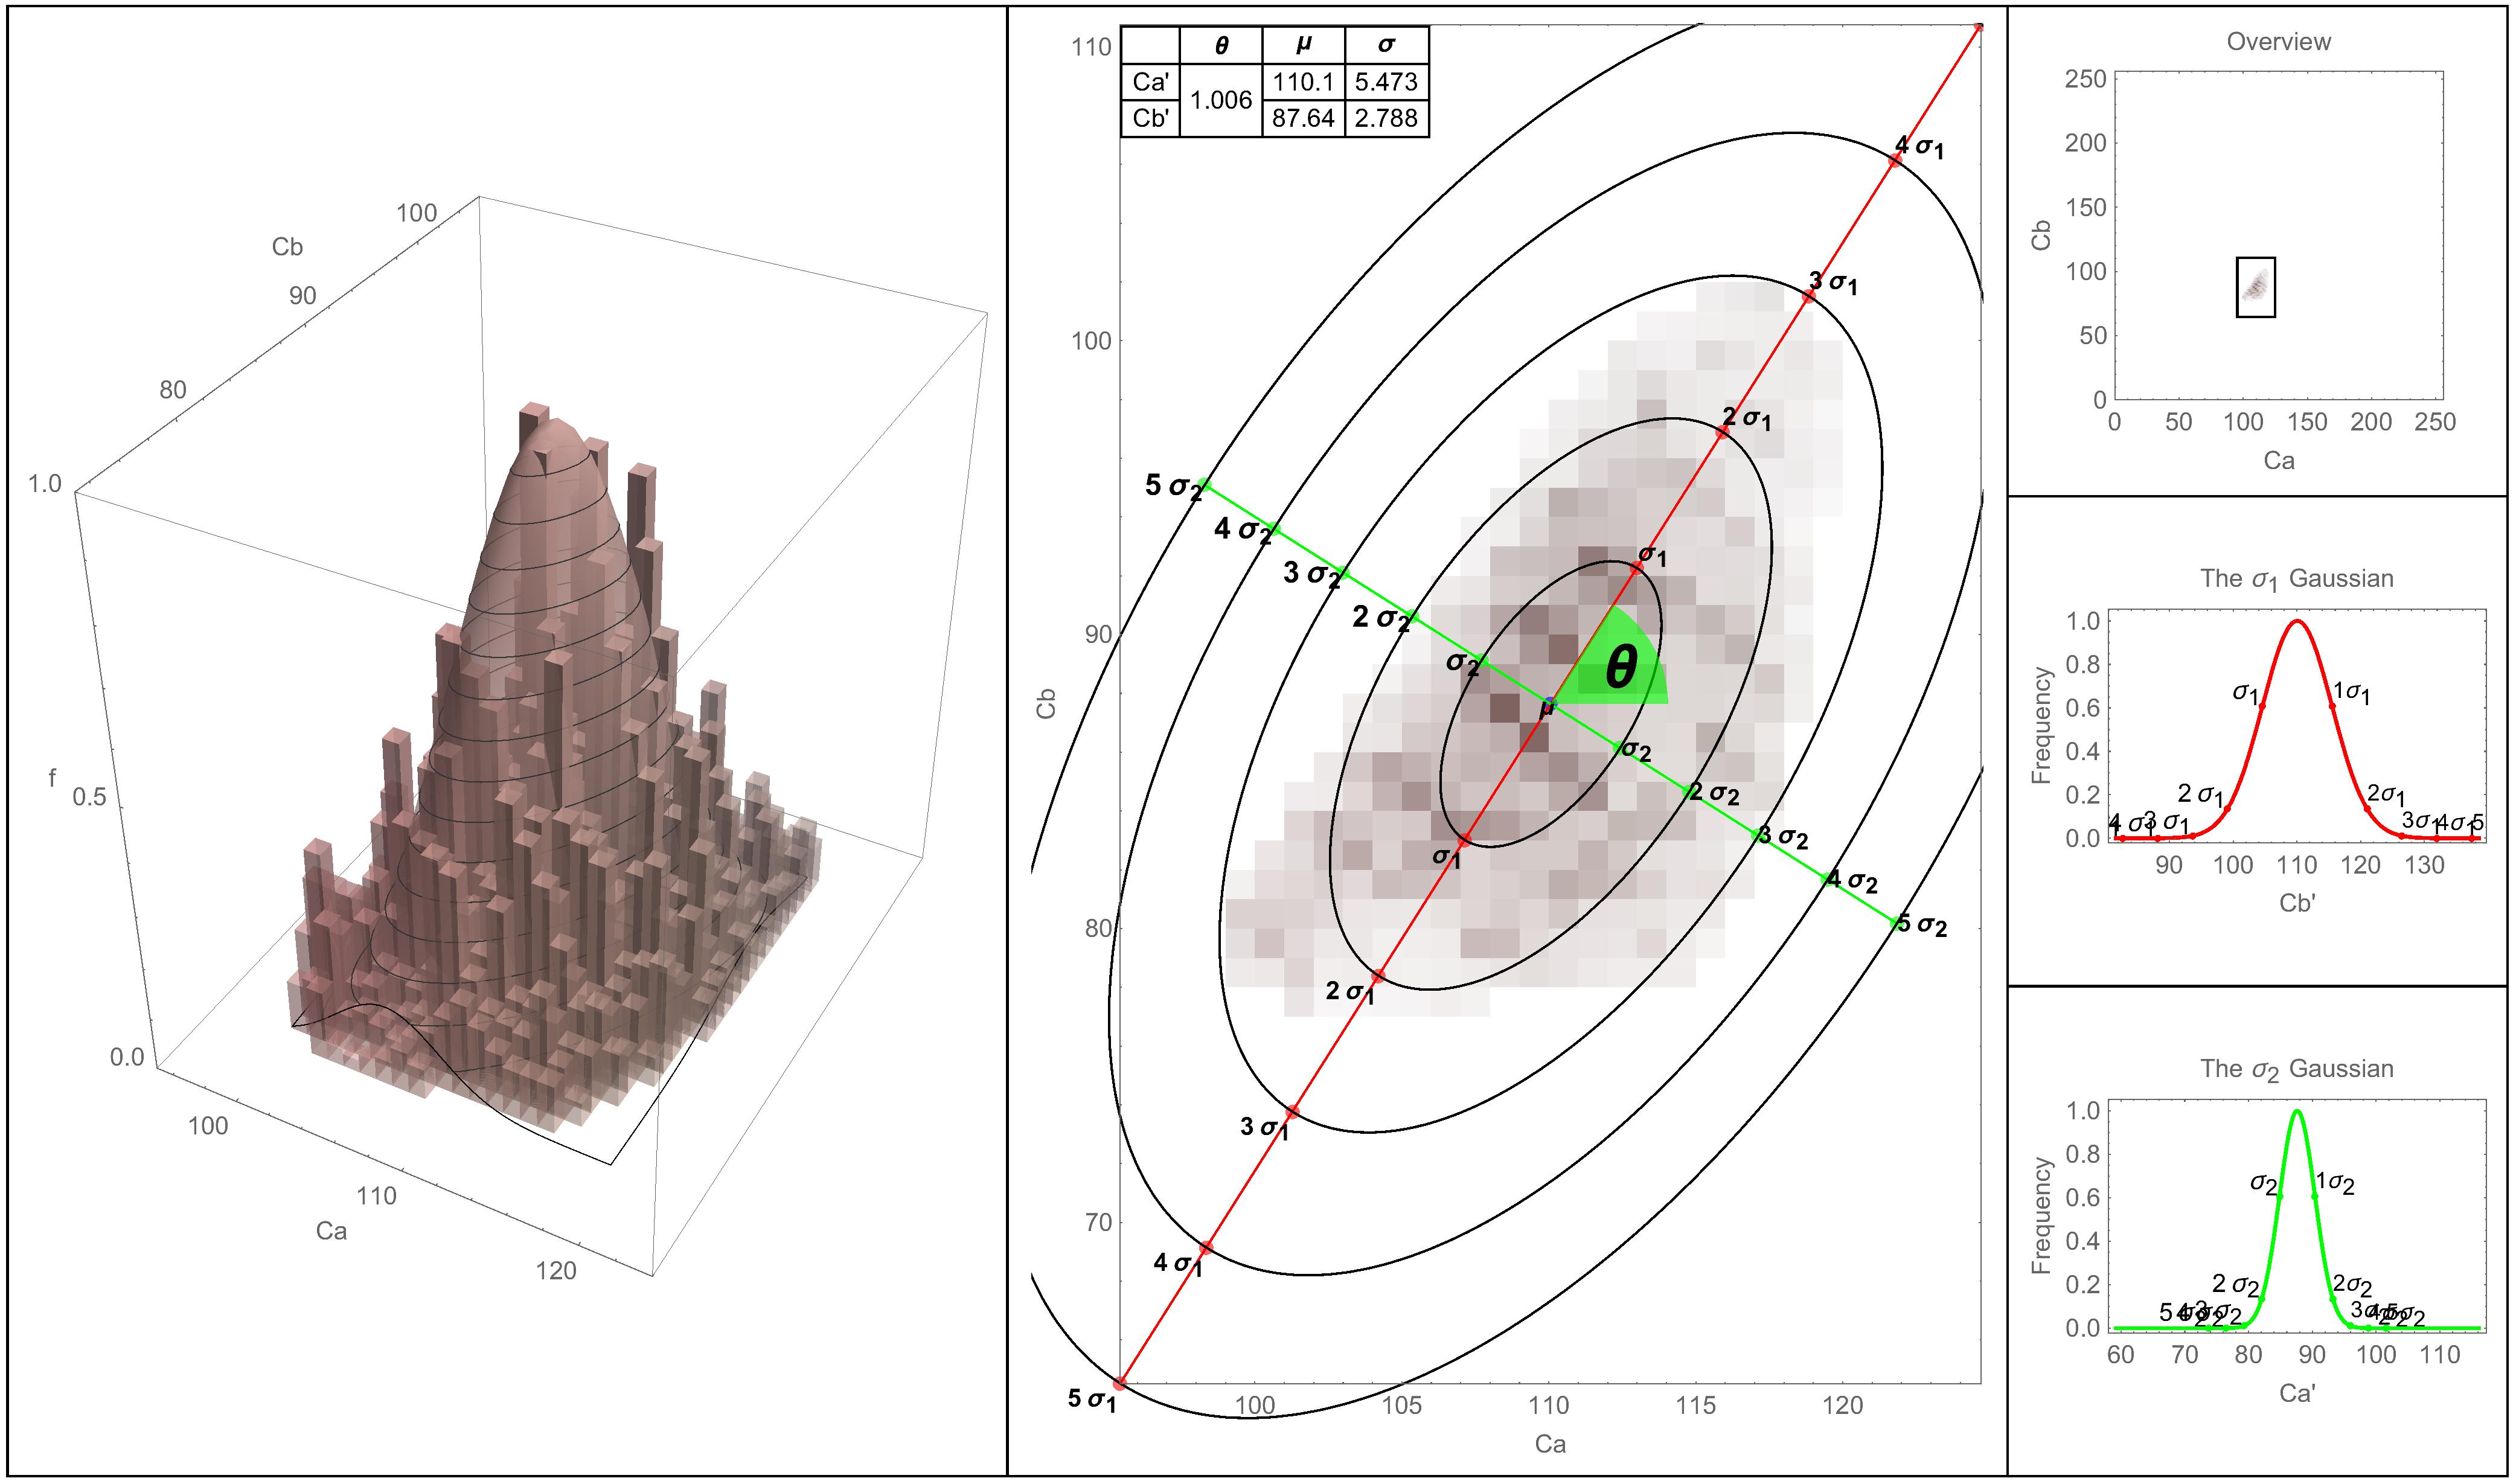
\includegraphics[width=1.0\textwidth]{Chapter3/Figs/\individual/Fit_the_Gaussian0.jpg}
        \caption{The Gaussian fit to the blob}  \label{fig:Fit_the_Gaussian0}
    \end{figure}


We now have a histogram which has bin values relevant to the target and no others. The elliptical blob fit values are used to initialize a 2D Gaussian fit to the normalized histogram. 

A least squares fit of the 2D Histogram with a 2D Gaussian function (Equation \ref{eq:2DGaussian}) is found using MATLAB's lsqcurvefit function.
\newcommand{\CaMu}{ \overline{\mathbf{Ca}} }
\newcommand{\CbMu}{\overline{\mathbf{Cb}}  }
\begin{equation}\label{eq:2DGaussian}
    \begin{gathered}
\textbf{Initialize} \quad \mu = \widetilde{\mu} \quad \sigma = \widetilde{\sigma} \quad \theta = \widetilde{\theta} \\
\textbf{ Perform Least Squares Fit Using:} \\
\textbf{Let} \quad \CaMu = \text{Ca}-\mu_1 \quad \text{and} \quad \CbMu = \text{Cb}-\mu_2 \\
\exp \left(
-\frac{\left( - \CaMu \; \sine{     \theta } + \CbMu \; \cosine{ \theta } \right){}^2}{2 \sigma_2^2} - 
\frac{\left(      \CaMu \; \cosine{ \theta } + \CbMu \; \sine{      \theta} \right){}^2}{2 \sigma_1^2} \right)
\end{gathered}
\end{equation}


\section{Sample Sets and Results}\label{sec:SampleSets}

\begin{figure}[h!]
  \centering
    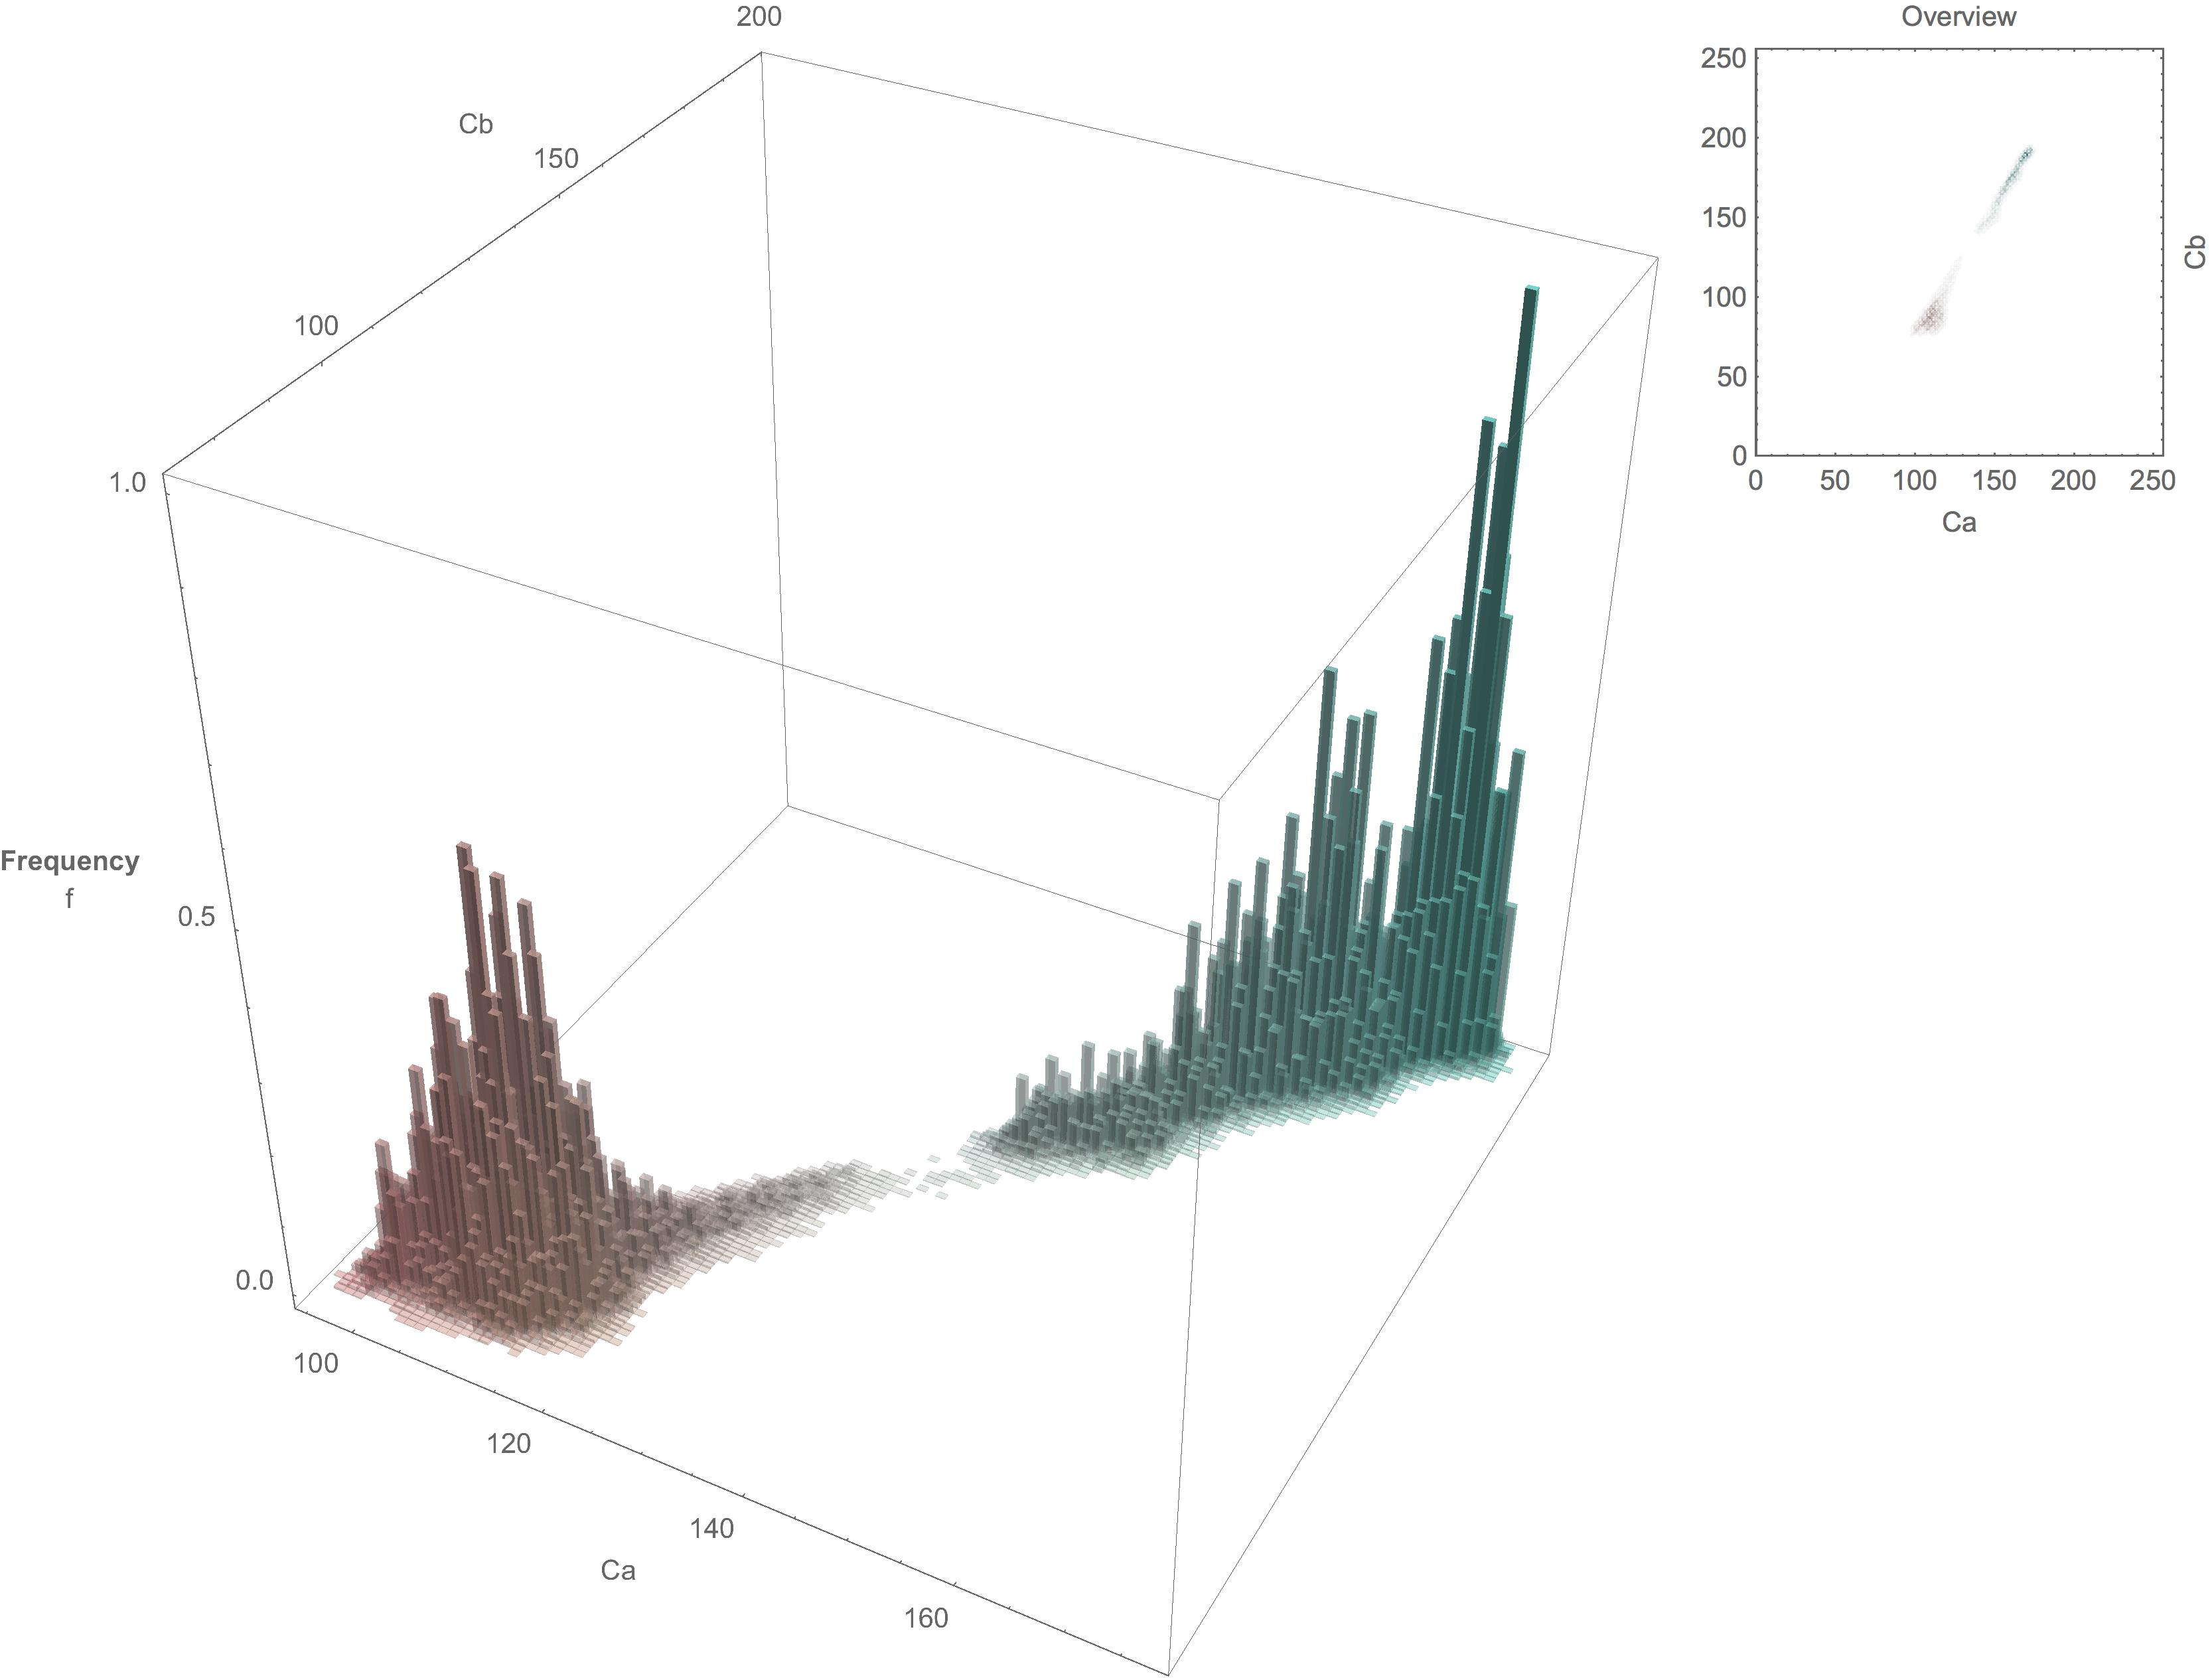
\includegraphics[width=1.0\textwidth]{Chapter3/Figs/\individual/Despeckle_the_Bins_Surf.jpg}
        \caption{The Ca Cb histogram for the combined F,J\&N sets incliding the background. The colors indicate the pixel color corresponding to the bin. }  \label{fig:Despeckle_the_Bins_Surf}
    \end{figure}

\begin{figure}[h!]
  \centering
    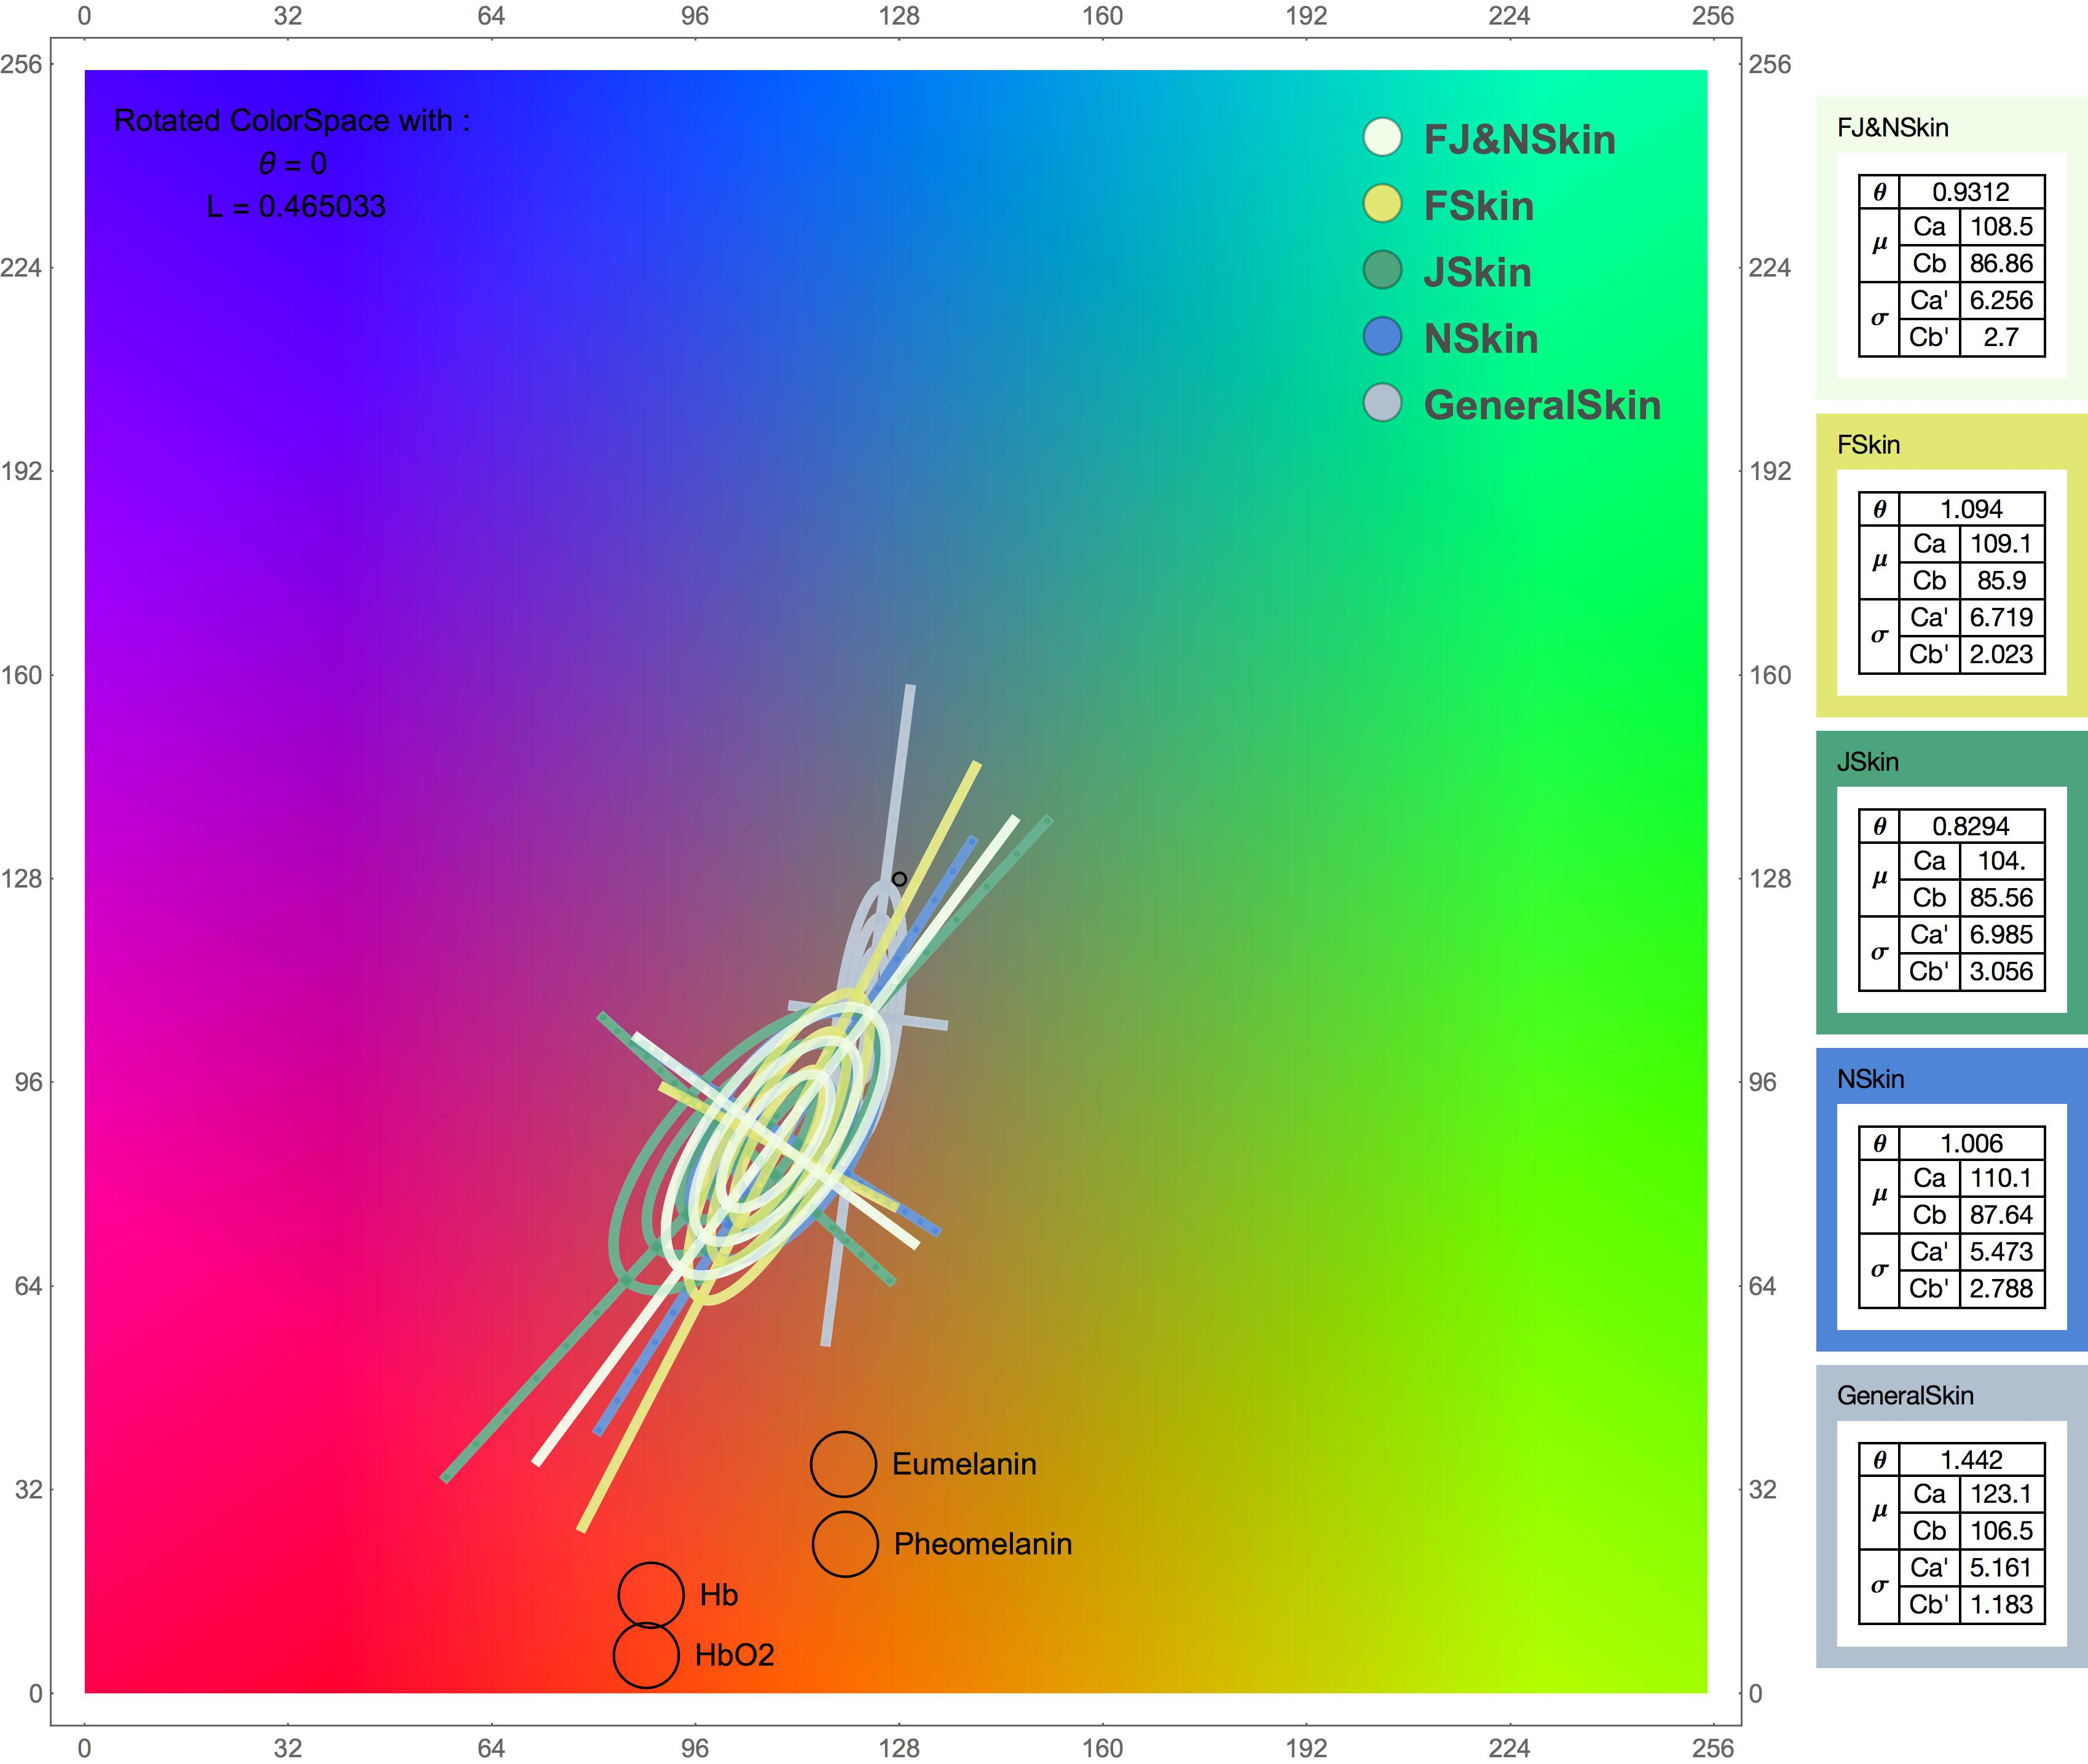
\includegraphics[width=\textwidth]{Chapter3/Figs/All_Together_2D.jpg}
    \caption{The four sets and the combined set of individuals. The ellipses are placed at $2\sigma$, $3\sigma$ and $4\sigma$ positions. Values inside $2\sigma$ would be kept by the distribution function.}  \label{fig:AllTogether2D}
\end{figure}


\begin{figure}[h!]
  \centering
    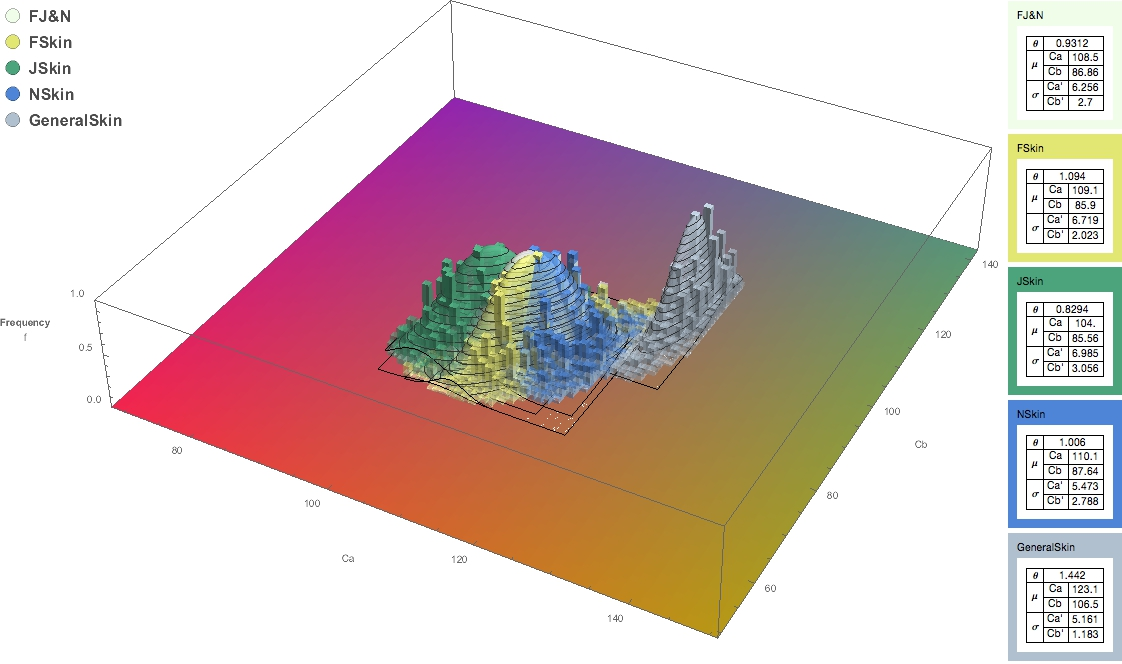
\includegraphics[width=\textwidth]{Chapter3/Figs/All_Together_3D.jpg}
    \caption{The histograms for the four data sets and the combined set of individuals are shown alongwith the Gaussian fits to the histogram. The color indicates the data set.}  \label{fig:AllTogether3D}
\end{figure}

Sample image sets were collected using the iPhone for three individuals with varying skin tones. Sets of images were taken for each digit and the hand as a whole under different lighting conditions and orientations. A selection of the images can be seen in Figure \ref{fig:SetSamples}.


\begin{figure}[h!]
  \centering
  \begin{tabular}{||c||c||c||}
  \hline \rule[-2ex]{0pt}{5.5ex}  FSkin &  JSkin & NSkin \\ 
  \hline \rule[-2ex]{0pt}{5.5ex} 
  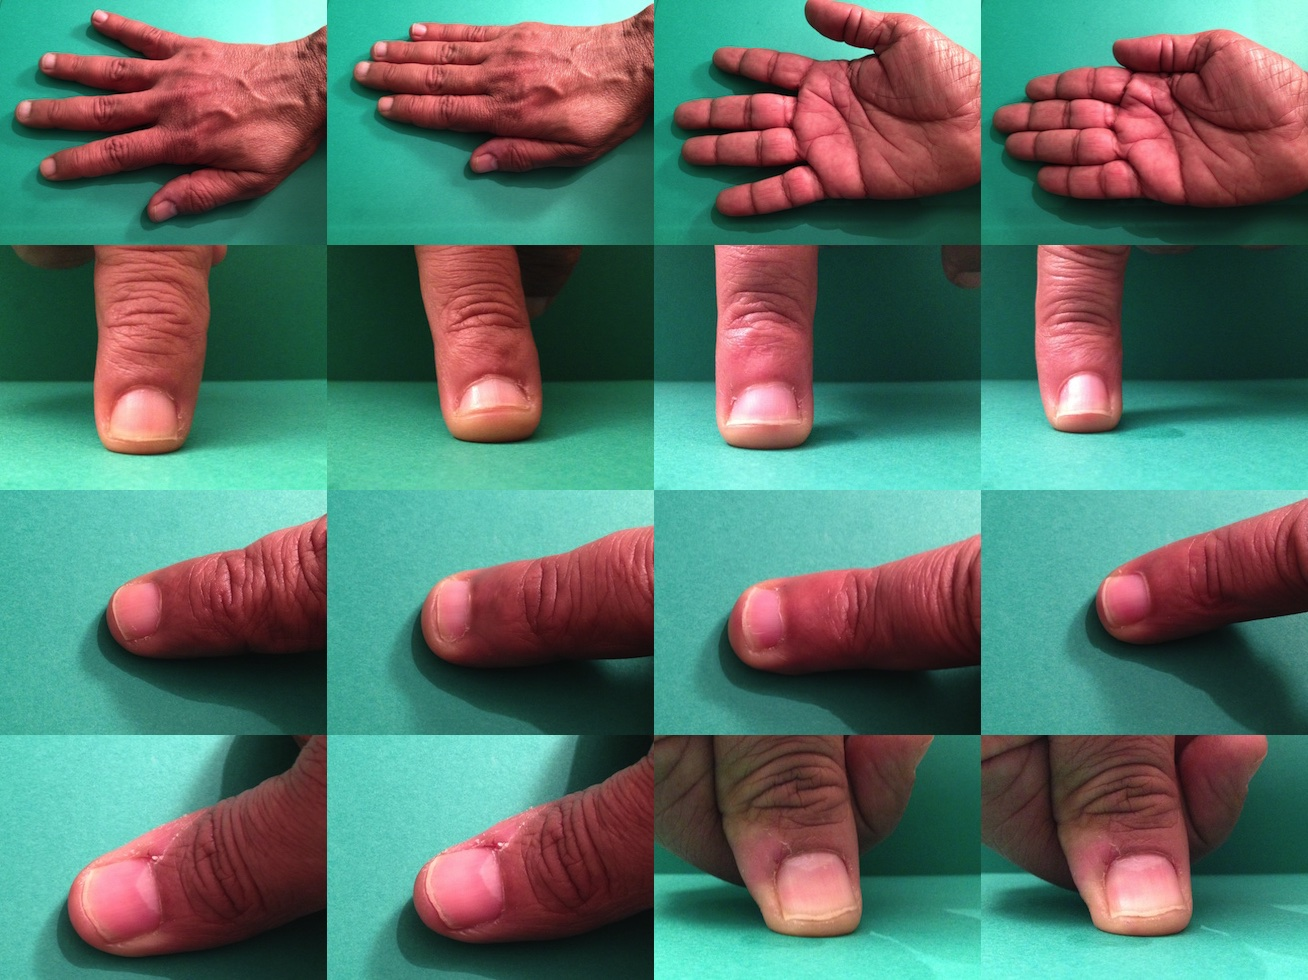
\includegraphics[width=0.3 \textwidth]{Chapter3/Figs/SampleCollages/FSkin_Sample.jpg} & 
  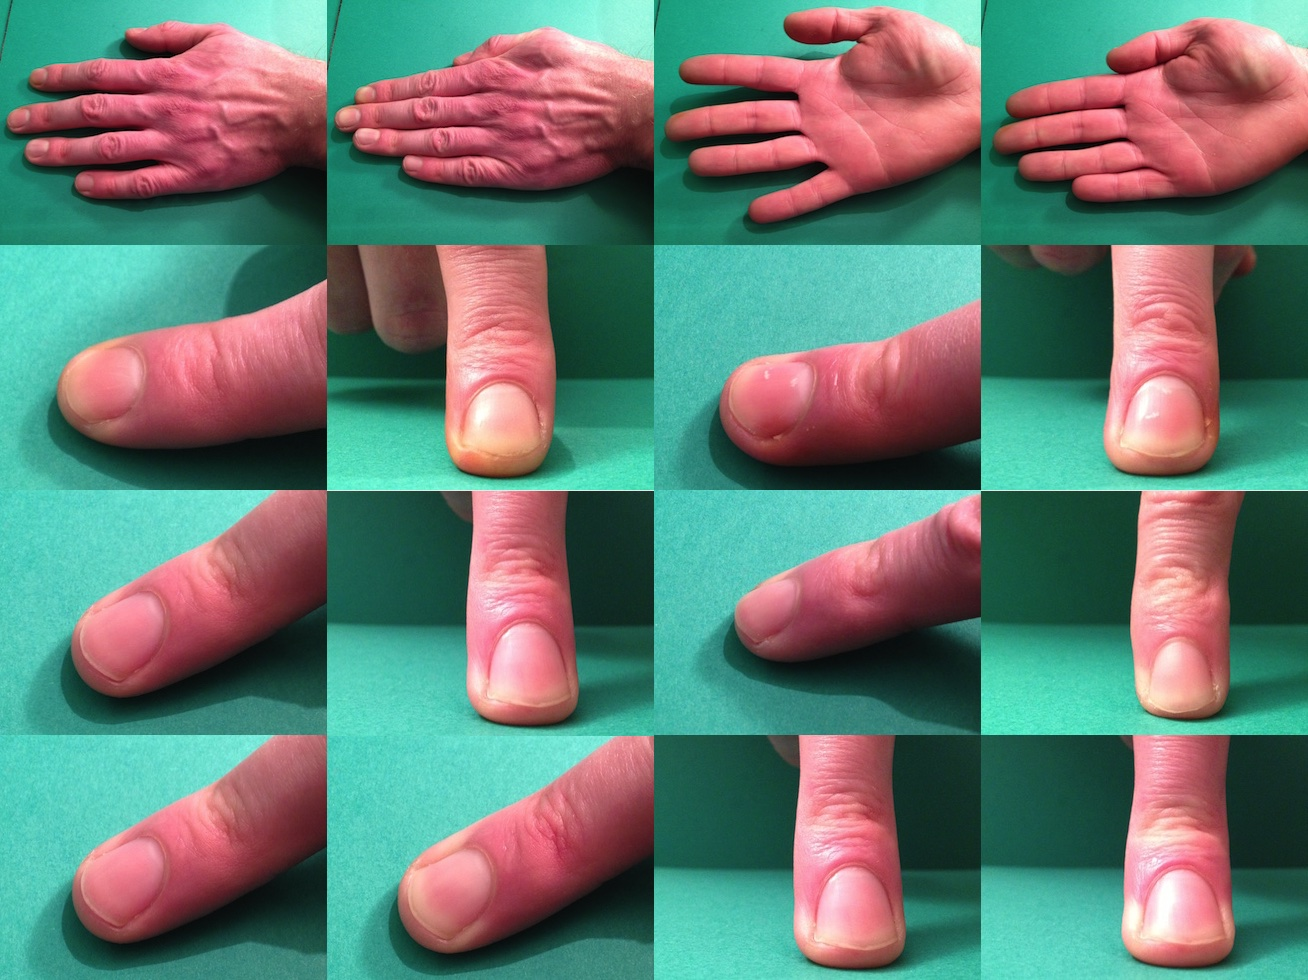
\includegraphics[width=0.3 \textwidth]{Chapter3/Figs/SampleCollages/JSkin_Sample.jpg} &  
  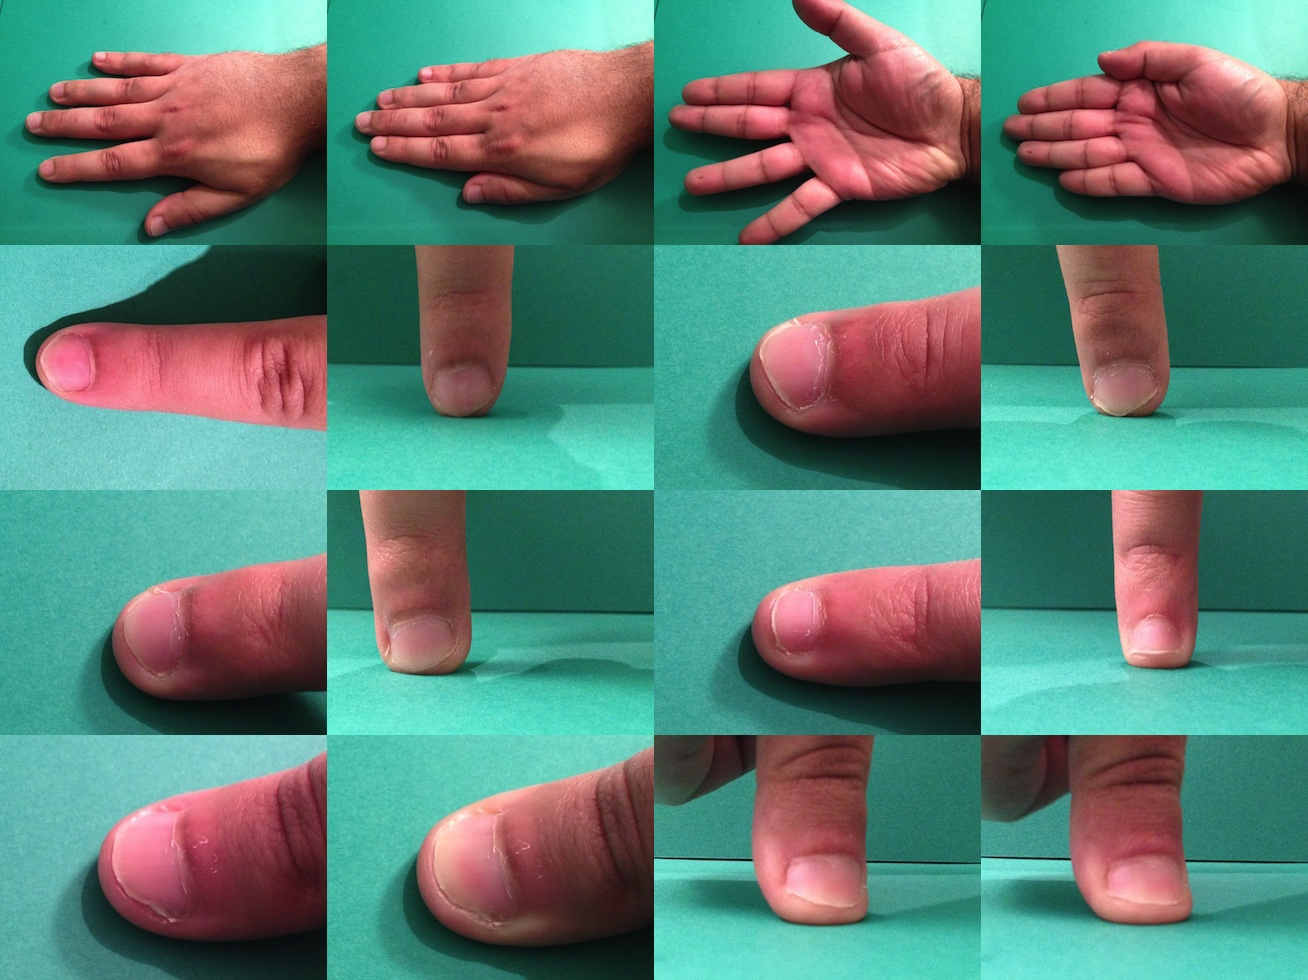
\includegraphics[width=0.3 \textwidth]{Chapter3/Figs/SampleCollages/NSkin_Sample.jpg}\\ 
  \hline 
  \end{tabular} 
    \caption{Samples from the image sets for each individual.}  \label{fig:SetSamples}
\end{figure}

The MATLAB bin class was written so that the combined statistics for the three individuals could be found by adding the RGB bins together, and then following the same steps 3.3.1-3.3.8 as described previously. All three distributions along with the combined distribution can be seen in Figures \ref{fig:AllTogether2D} and \ref{fig:AllTogether3D}.


In an attempt to identify a larger range of values for the skin space, a large number of skin samples were taken from photographs from the Humane project by Angelica Dass, an ongoing "chromatic inventory" art project which aims to compile every possible human skin color, categorized by the PANTONE guide color classification system~(\cite{Dass2012}). The skin colors catalogued thus far are independent of race or ethnicity, so the samples are representative of human skin tones in general.

The image set consists of approximately 200 skin samples  each showing only one individuals skin. The result can be seen in Figures \ref{fig:AllTogether2D} and \ref{fig:AllTogether3D} as the GeneralSkin set. The distribution stands apart from the others and surprisingly has a smaller standard deviation. This is probably due to camera differences and the sampling techniques used in the Humane project which focus on finding an average color rather than the channel values in camera. The orientation and position of the distribution is more consistent with the theoretical values for the skin pigments than those for the individual sets. This is likely due to the fact that the theoretical values were calculated for a different camera CCD, the iPhone CCD characteristics not being available. For this reason the general distribution is excluded from further consideration aside from the recognition that different cameras will require bespoke statistics to be gathered. 

In contrast to the GeneralSkin set the individual sets are close together with similar standard deviations, however the angle varies significantly. The angle needs to be fixed so that the statistics can be gathered in the rotated color-space. The angles are summarized in the table below:

\begin{tabular}{|c|c|c|c|}
\hline   Set                                                             & Decimal   & Approx                       & Relative \\ 
\hline   $\text{FJ$\&$NSkin }\theta _{\text{FJN}}$ & $0.9312$ & $\frac{75 \pi }{253}$ & $\theta _{\text{FJN}}$ \\
\hline   $\text{FSkin }\theta _F$                            & $1.0940$ & $\frac{39 \pi }{112}$ & $\theta _{\text{FJN}}+\frac{3 \pi }{58}$ \\
\hline   $\text{JSkin }\theta _J$                             & $0.8294$ & $\frac{33 \pi }{125}$ & $\theta _{\text{FJN}}-\frac{\pi }{31}$ \\
\hline   $\text{NSkin }\theta _N$                          & $1.0060$ & $\frac{49 \pi }{153}$ & $\theta _{\text{FJN}}+\frac{\pi }{42} $\\
\hline 
\end{tabular} 

This suggests that taking $\theta'$ to be in the range $\theta _{\text{FJN}} -\frac{\pi}{84} < \theta' < \theta _{\text{FJN}} +\frac{\pi}{84}$ is safe as it is, at most, half way to the nearest individual and the position of the mean remains within 2 standard deviations 
$\left(\begin{array}{c} 84 \\ 117 \end{array} \right) < \mu'  < \left(\begin{array}{c} 83 \\ 121 \end{array} \right) $. This is somewhat arbitrary and we could extend the region if we had reason but this range is sufficient to ensure that a computationally advantageous value will be within the range being 1/7th of a Pi/6 region.  The perturbation to the channels for the range of possible $\theta'$ values can be seen in Figures \ref{fig:PerturbationNearThetaAB} and \ref{fig:PerturbationNearThetaT}.


\begin{figure}[h!]
  \centering
  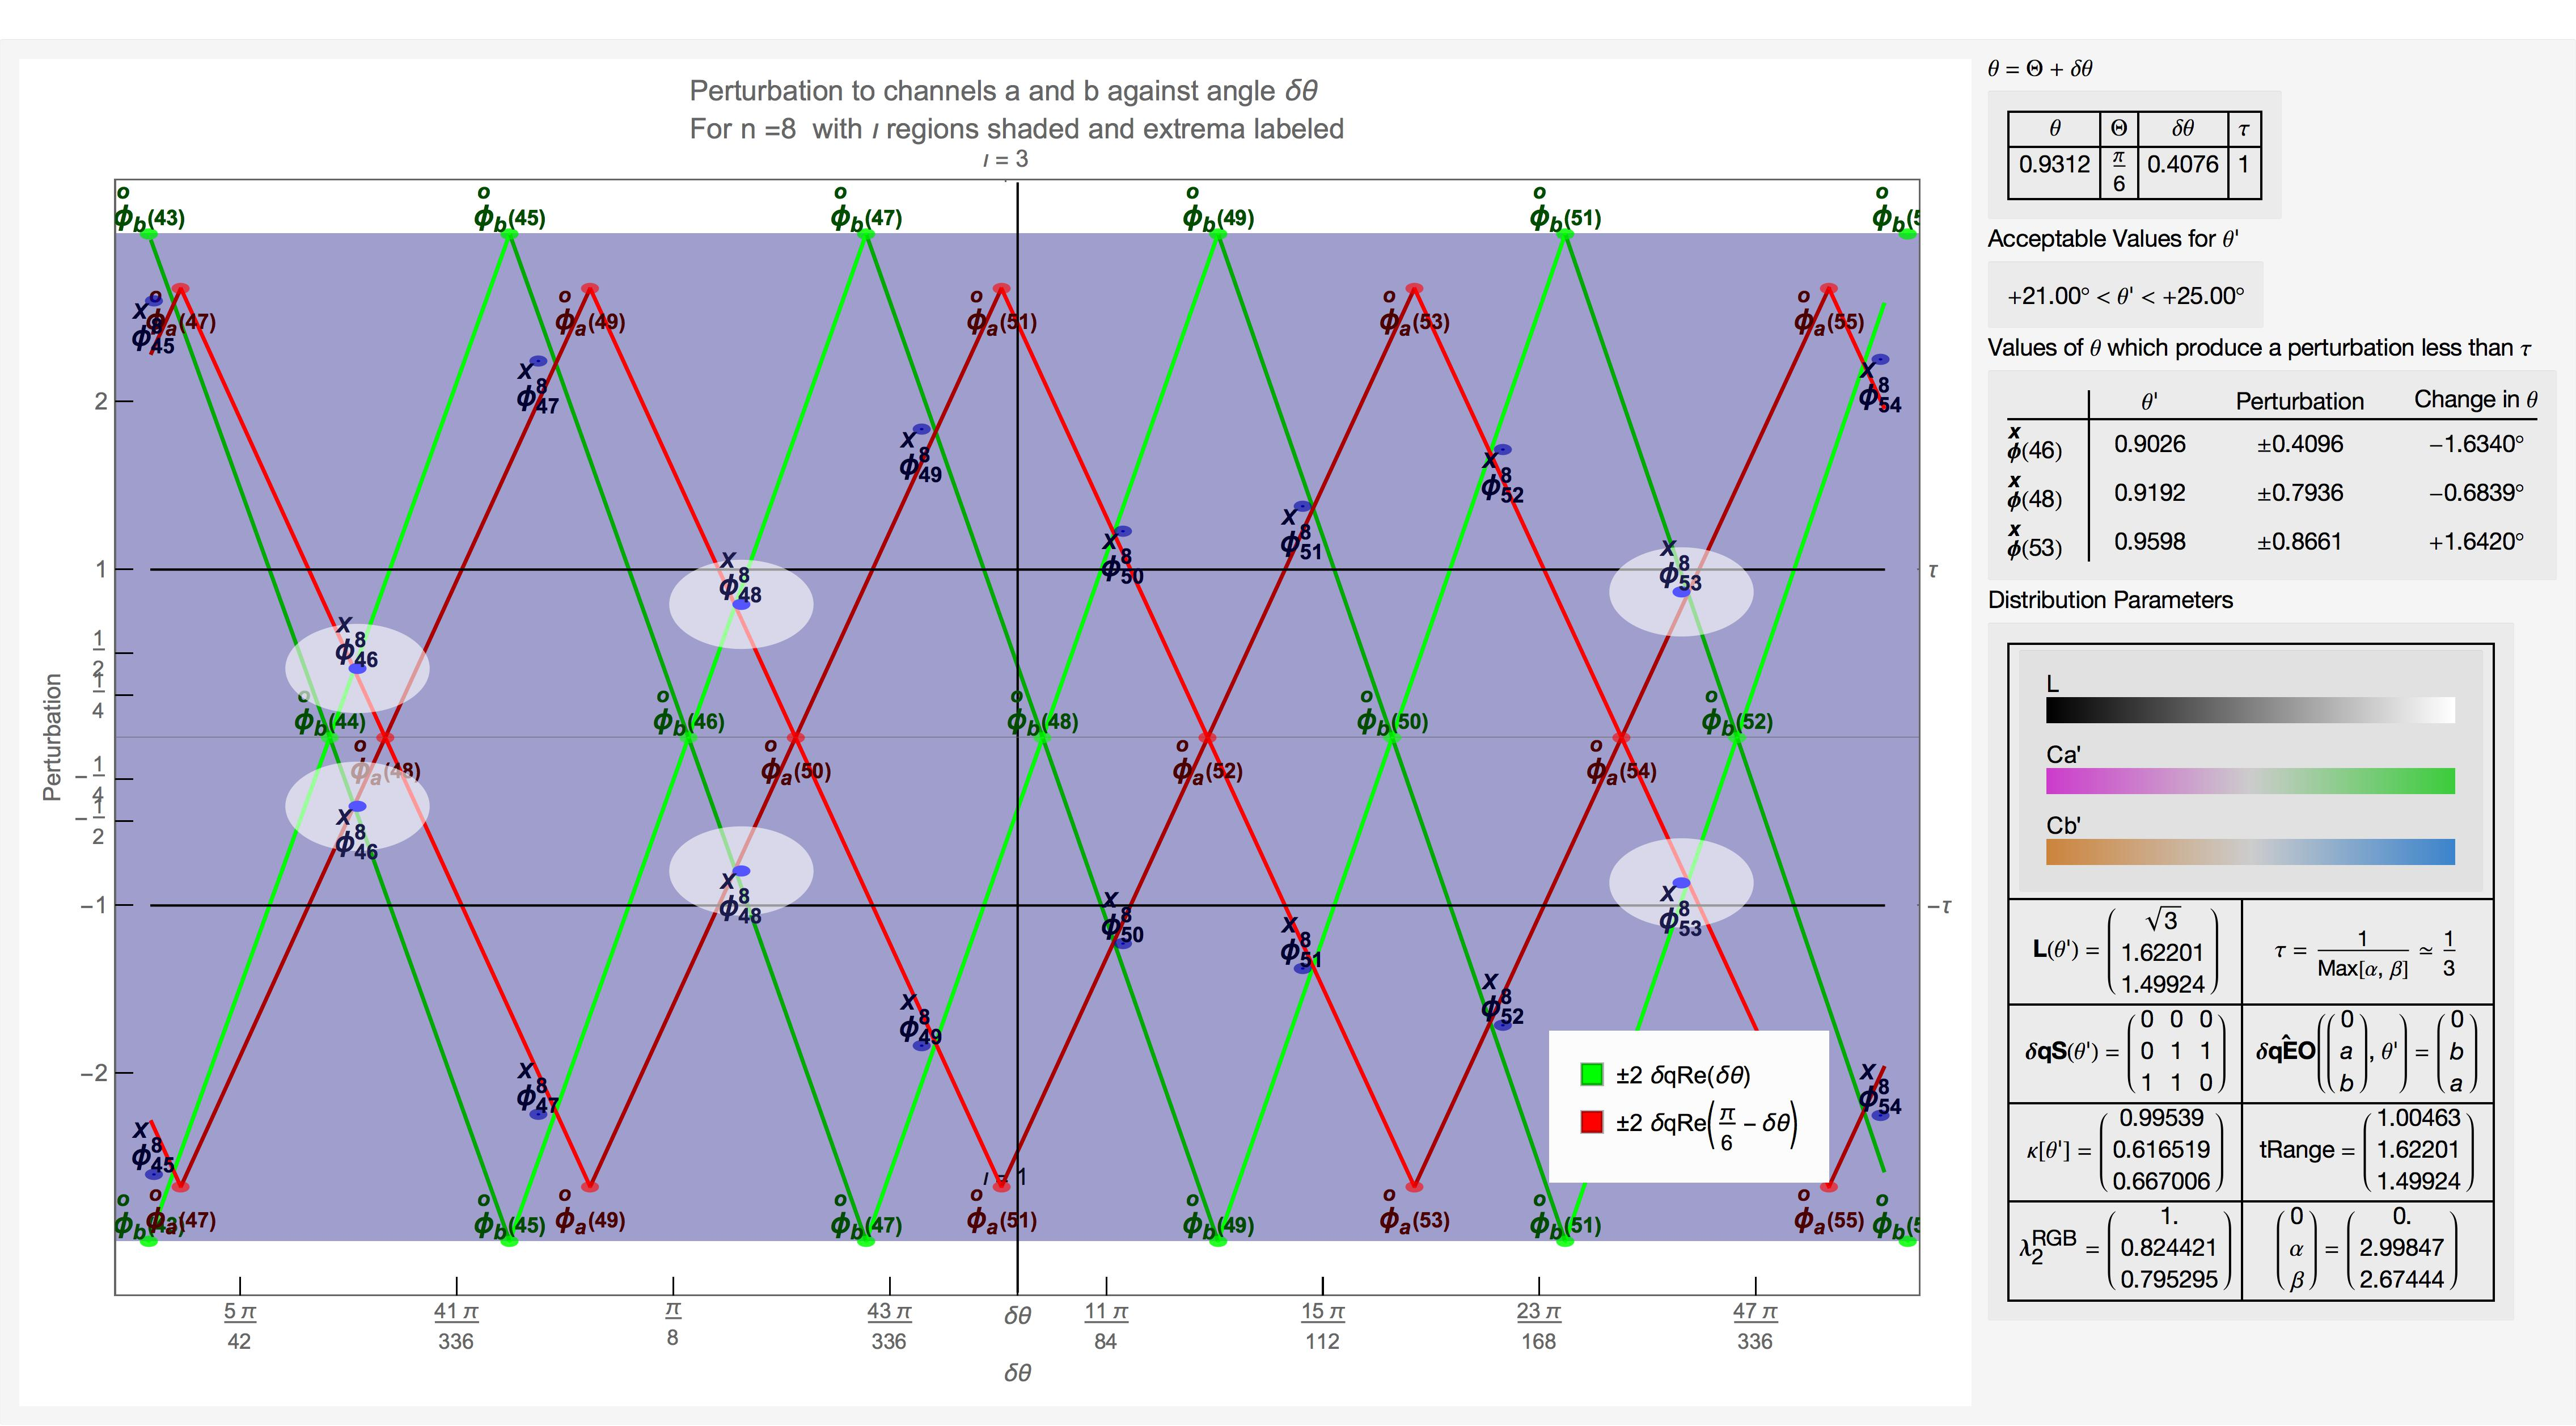
\includegraphics[width=1.0 \textwidth]{Chapter3/Figs/Channel_Perturbations_Angle_Decision_AB.jpg} 
    \caption{The channel perturbations within $\frac{\pi}{84}$ of $\theta'$. The channel perturbations are scaled by $\alpha$ and $\beta$ so a tolerance $\tau=1$ is used. Three angles satisfy the requirements}  \label{fig:PerturbationNearThetaAB}
\end{figure}

\begin{figure}[h!]
  \centering
  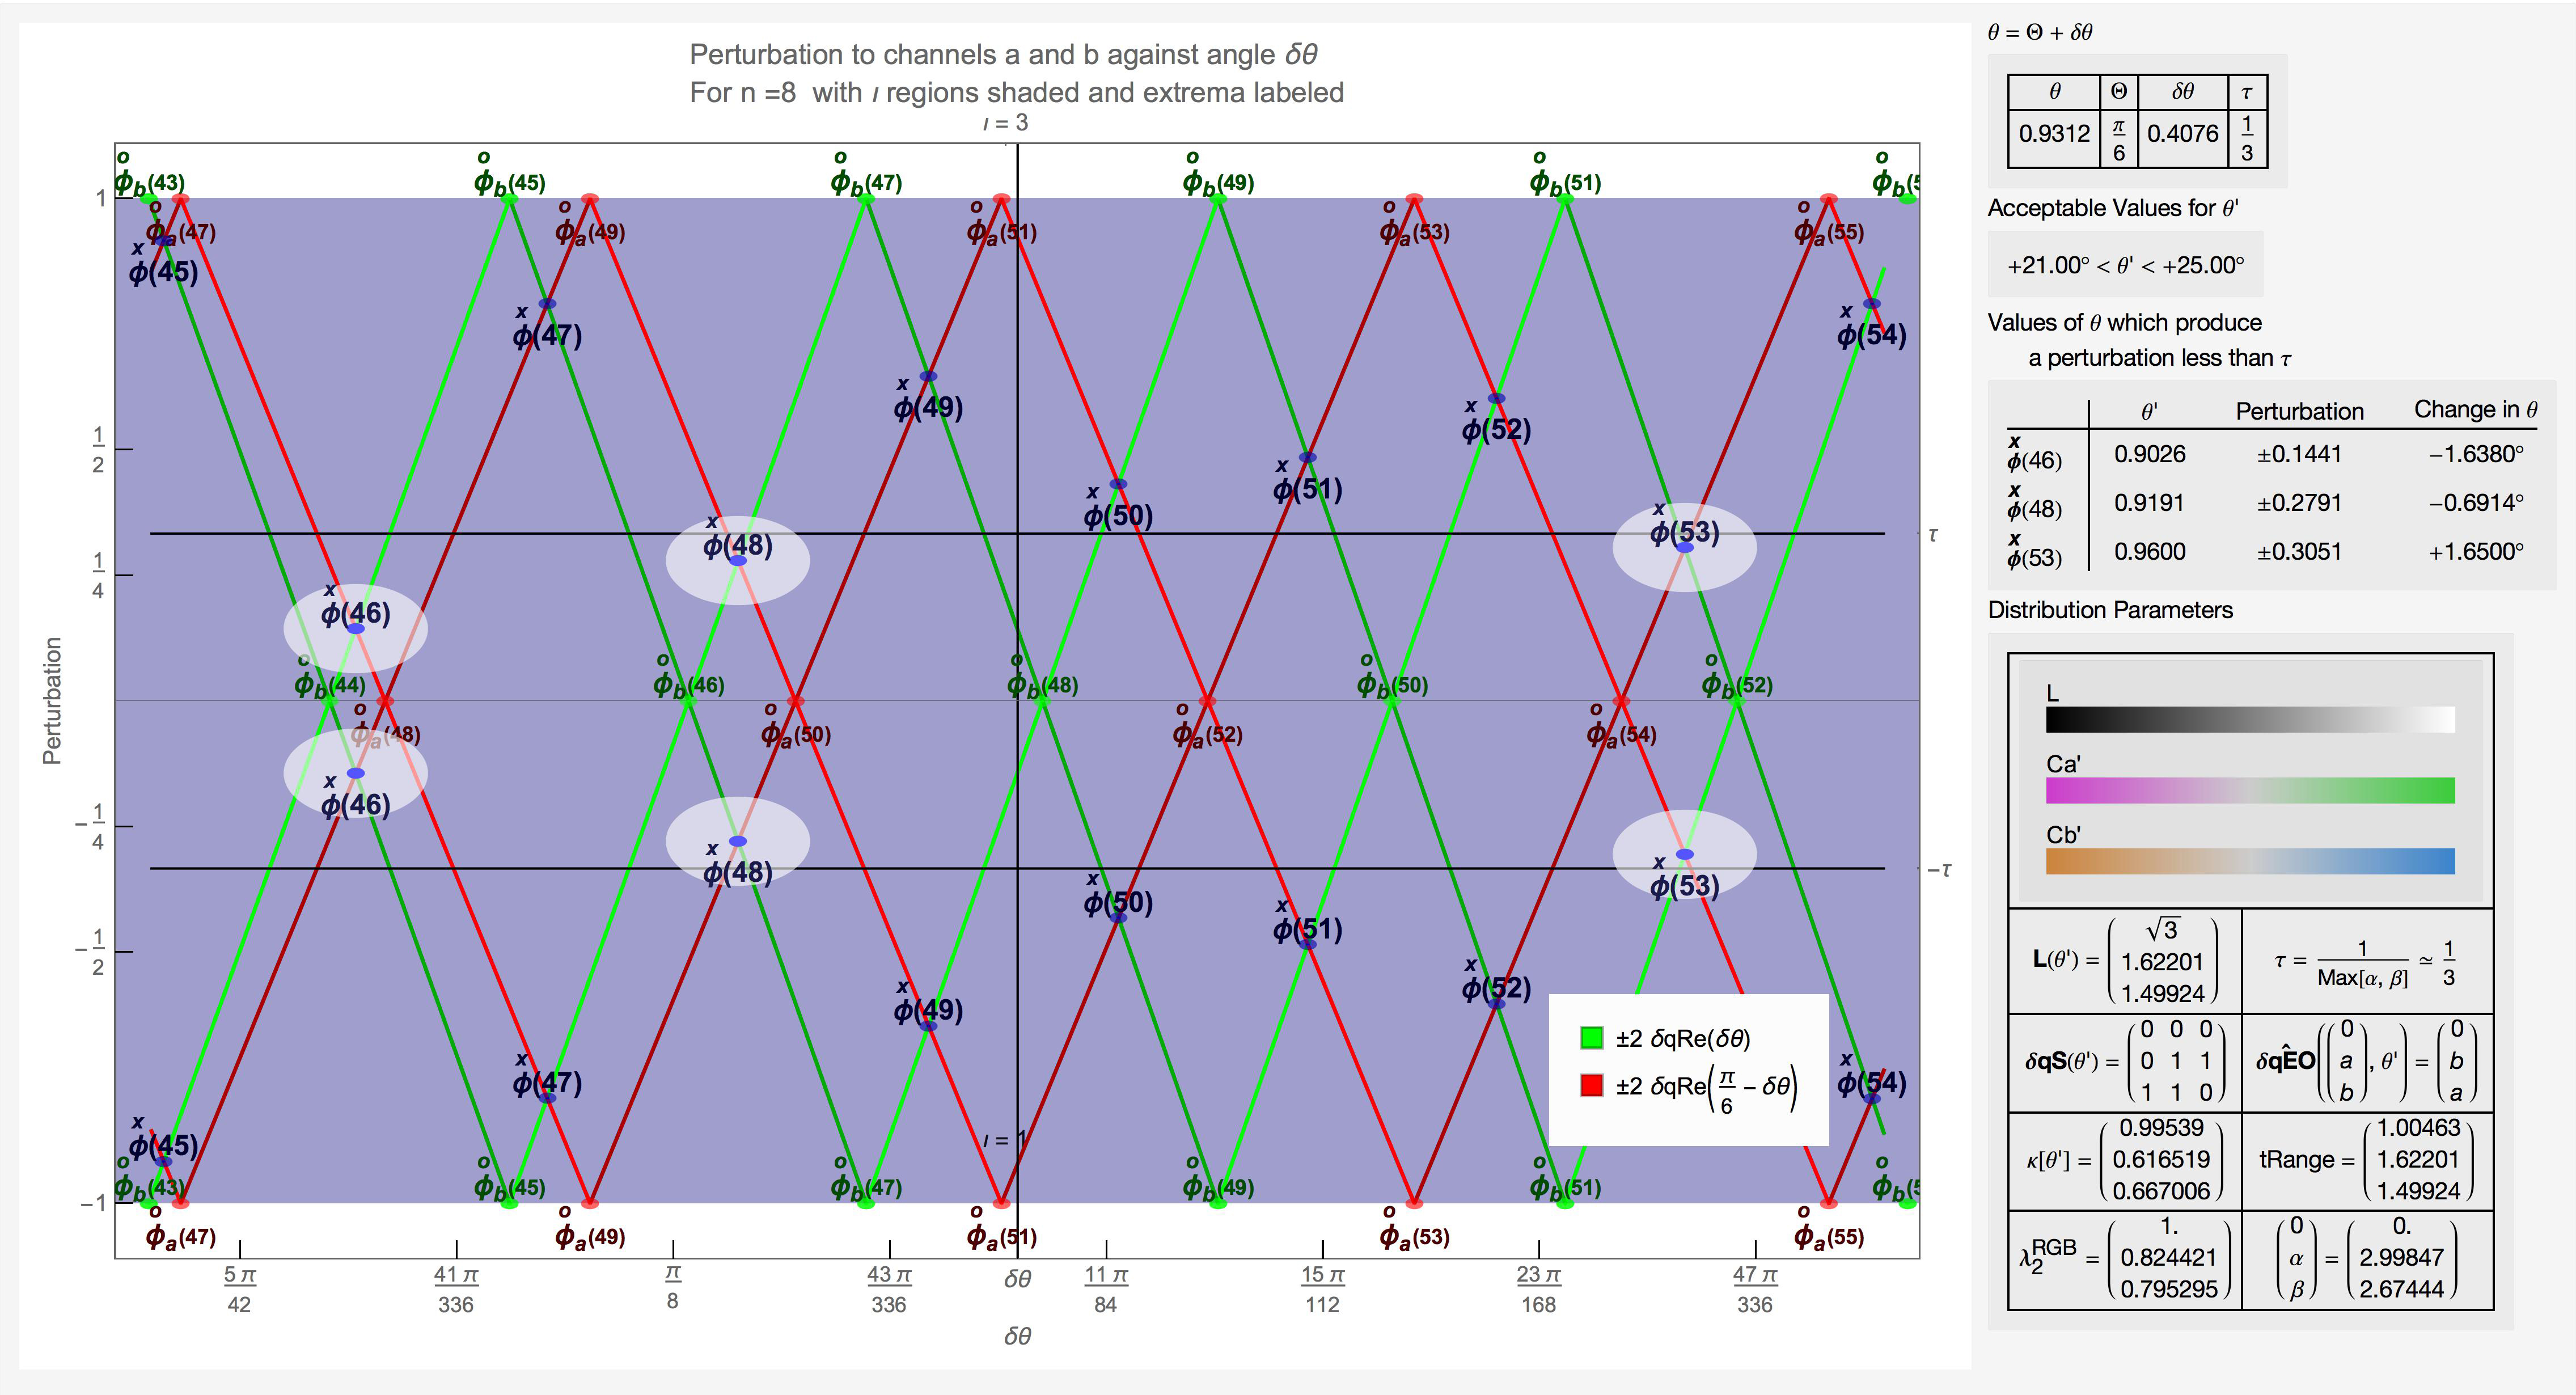
\includegraphics[width=1.0 \textwidth]{Chapter3/Figs/Channel_Perturbations_Angle_Decision_T.jpg} 
    \caption{The channel perturbations within $\frac{\pi}{84}$ of $\theta'$.}  \label{fig:PerturbationNearThetaT}
\end{figure}

We now follow the procedure outlined in Chapter 2 and obtain an angle informed by computational considerations.  
With the perturbations to each channel scaled by their relative importance (Figure \ref{fig:PerturbationNearThetaAB}) there are three angles which satisfy the criteria.
 The algorithm returns the closest angle to the requested angle which is $\overset{x}{\phi } (48)$ however the perturbation is close to the tolerance of 1, which suggests that if the distribution parameters were adjusted to fit a particular individual then the perturbation may slip above the tolerance. 
 The channel scaling $\left\{ \alpha, \beta\right\} $ are also fairly close in value so the unscaled perturbations can be used with a tolerance $\tau = \text{Max}\left(\alpha, \beta\right)$ (Figure \ref{fig:PerturbationNearThetaT}). 
 Accounting for both low perturbation and future adaptability a final angle $\theta = \overset{x}{\phi }(46) = 0.9025768293268257$ was chosen.

\begin{figure}[h!]
  \centering
  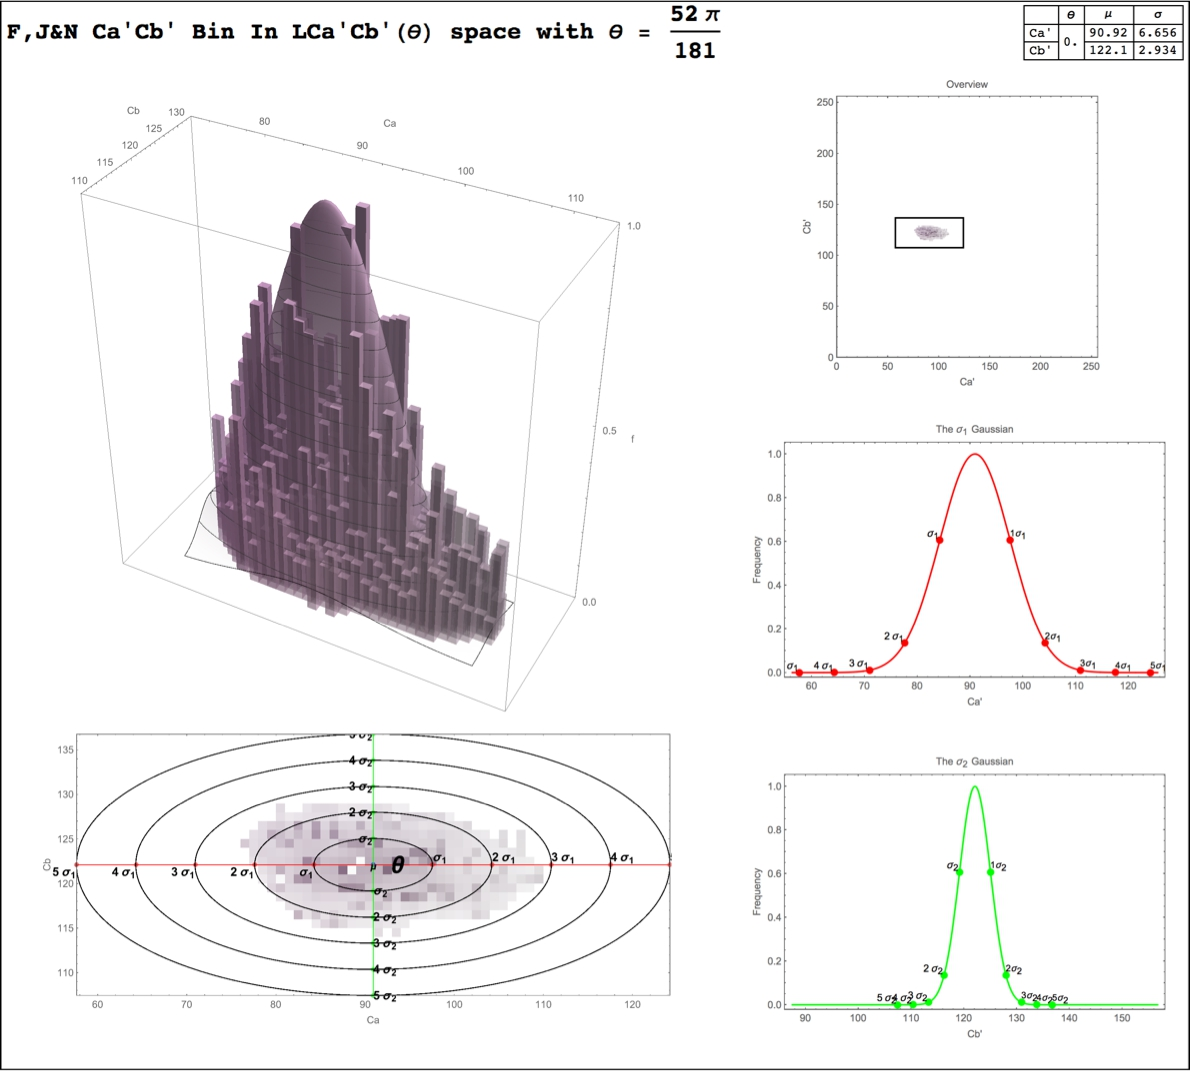
\includegraphics[width=1.0 \textwidth]{Chapter3/Figs/Fit_the_Gaussian_Final.jpg} 
    \caption{The Product of Gaussians fit to the three individuals statistics in the LCa'Cb' color-space.  }  \label{fig:FittheGaussianFinal}
\end{figure}

\begin{figure}[h!]
  \centering
  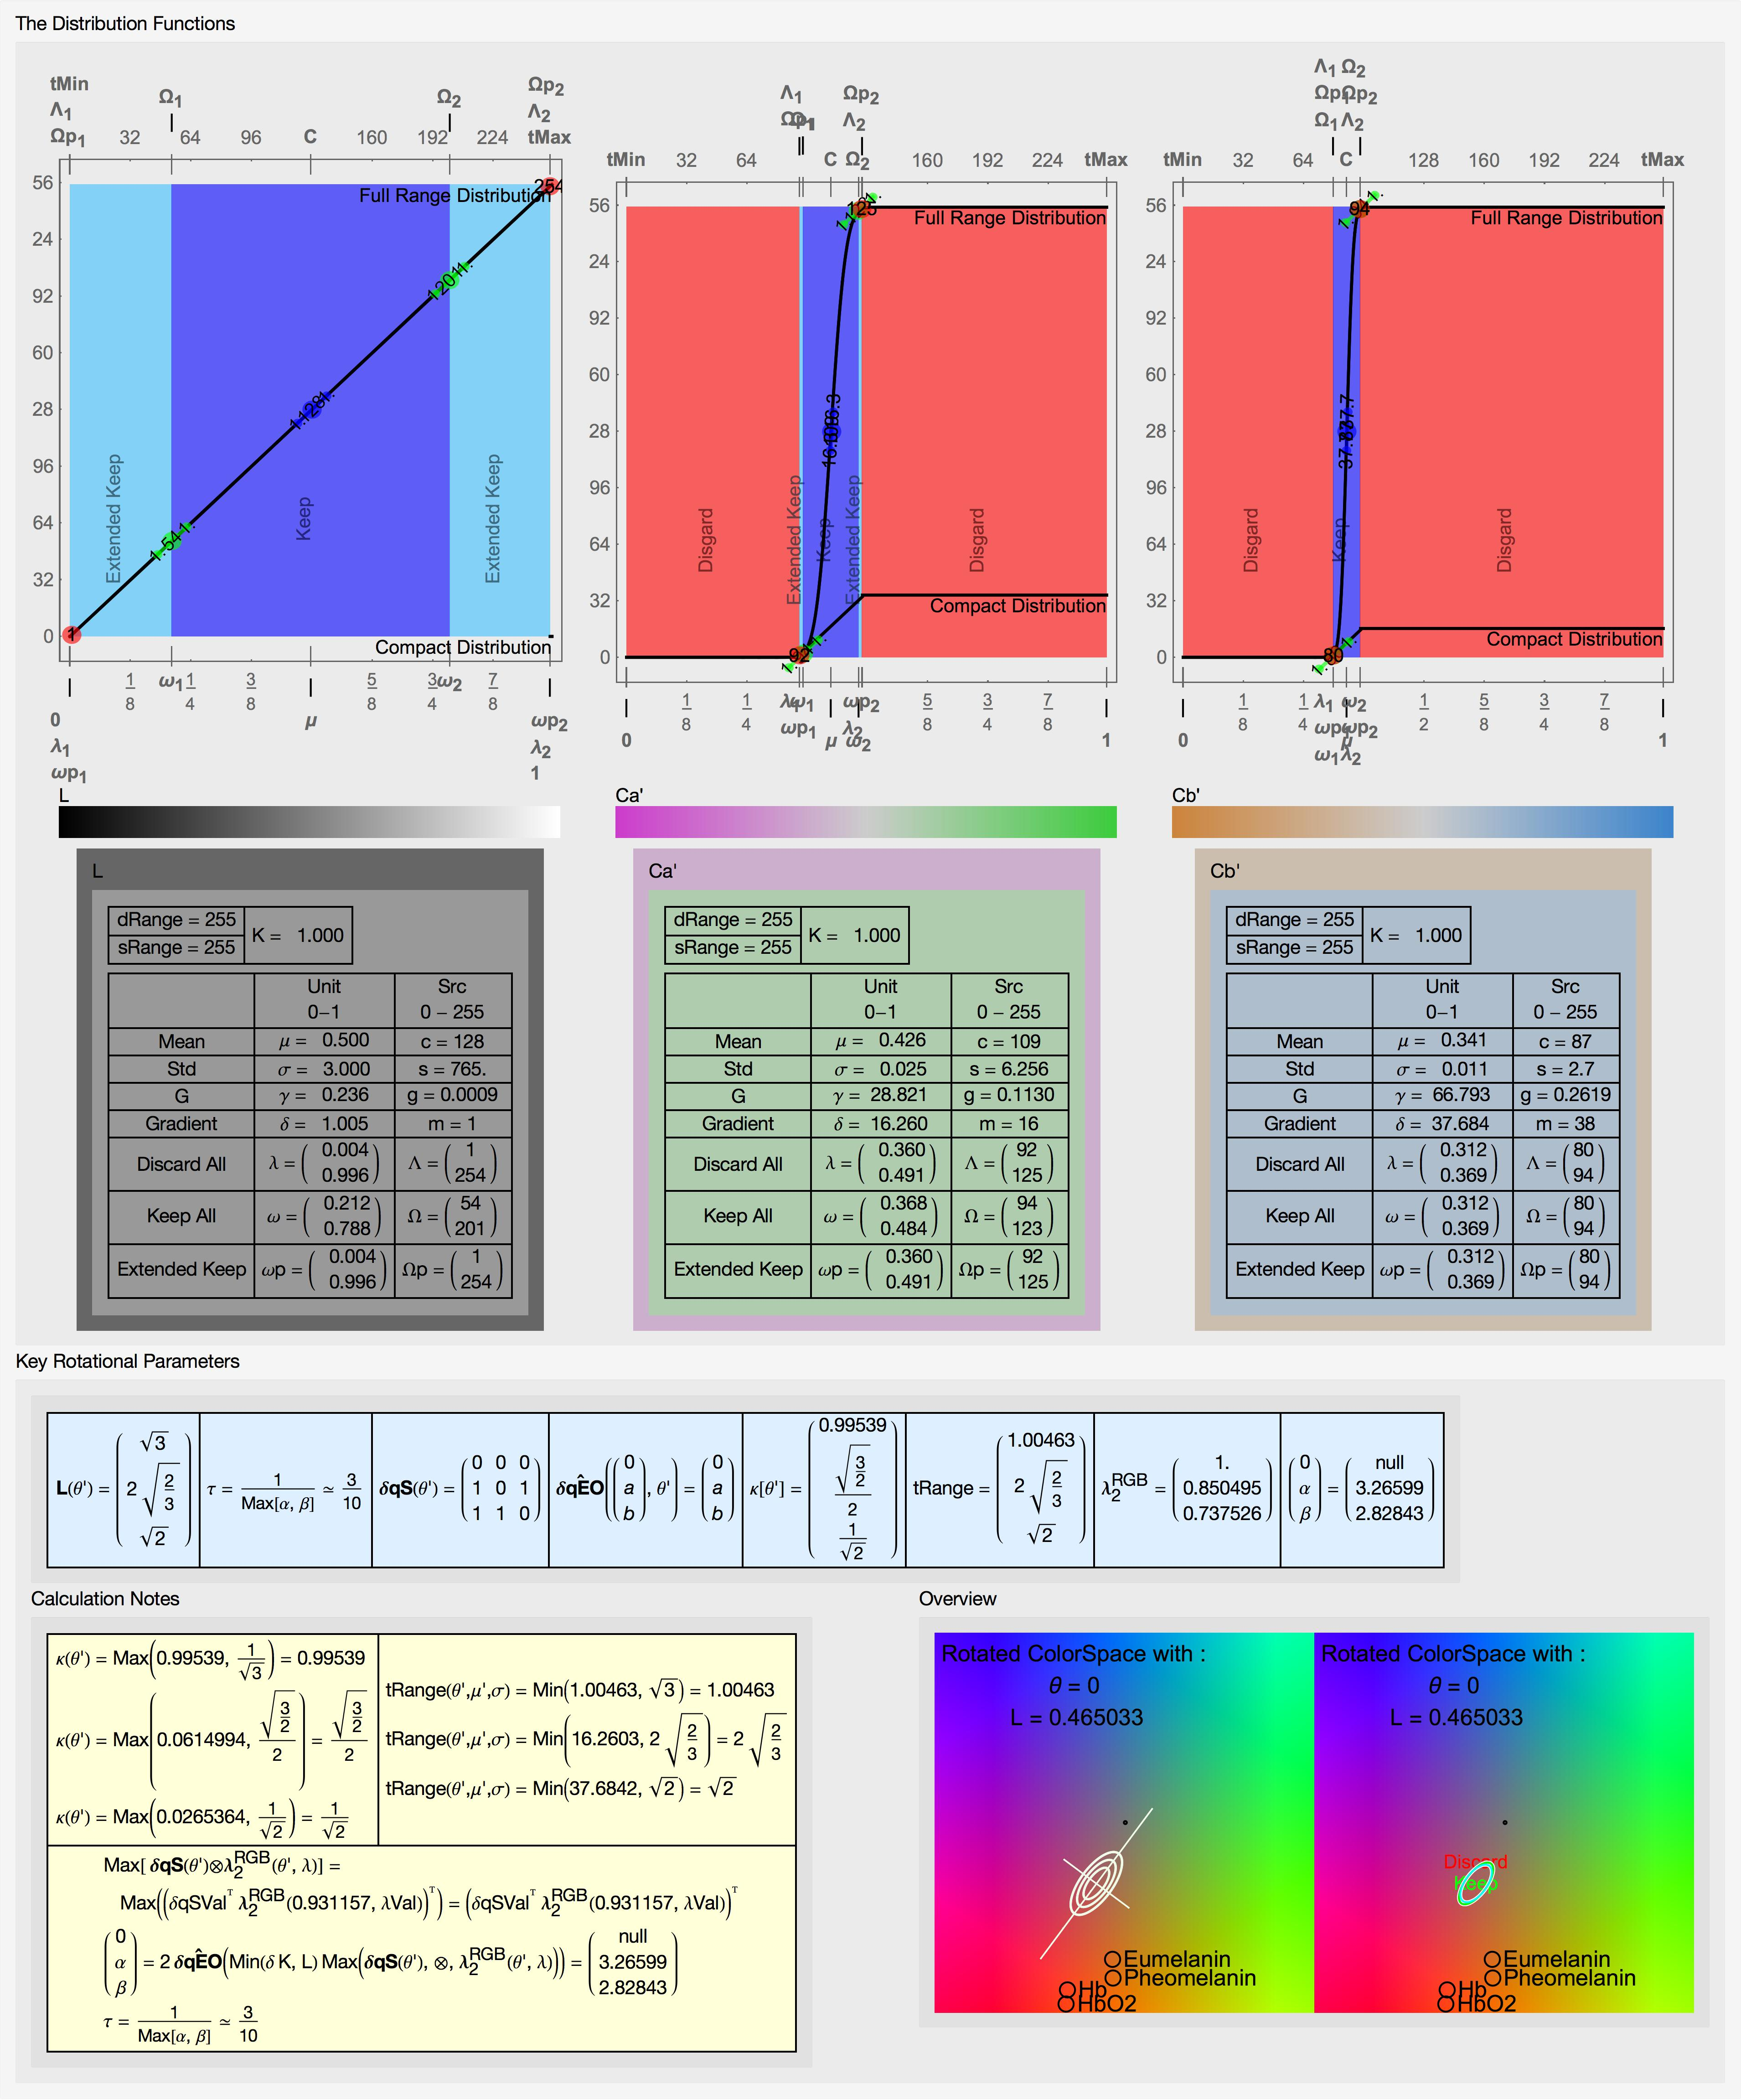
\includegraphics[width=1.0 \textwidth]{Chapter3/Figs/Distribution_Results.jpg} 
    \caption{ The redistribution functions for each axis alongside summary tables of the key parameters and a selection of calculations and an overview of the distribution in the new color-space  }  \label{fig:DistributionResults}
\end{figure}

As a final step, the MATLAB statistics gathering routine was run again using the combined F,J\&N RGB bins as a starting point and then rotating to the LCa'Cb' color-space with the new value for $\theta$. This was done partly to check that the code works as expected and to see how well the product of Gaussians function fits the distribution. The only difference to the MATLAB code was that for this run the Gaussian fit was found using Equation \ref{eq:2DGaussianProd} which is the product of two 1D Gaussians with a fixed Amplitude of 1. The result can be seen in Figure \ref{fig:FittheGaussianFinal}. 

\begin{equation}\label{eq:2DGaussianProd}
\exp \left( -\frac{{\CaMu}^2}{2 \sigma_1^2} -  \frac{ { \CbMu }^2}{2 \sigma_2^2} \right) \quad \textbf{where} \quad \CaMu = \text{Ca}-\mu_1 \quad \text{and} \quad \CbMu = \text{Cb}-\mu_2 
\end{equation}



\begin{figure}[h!]
  \centering
  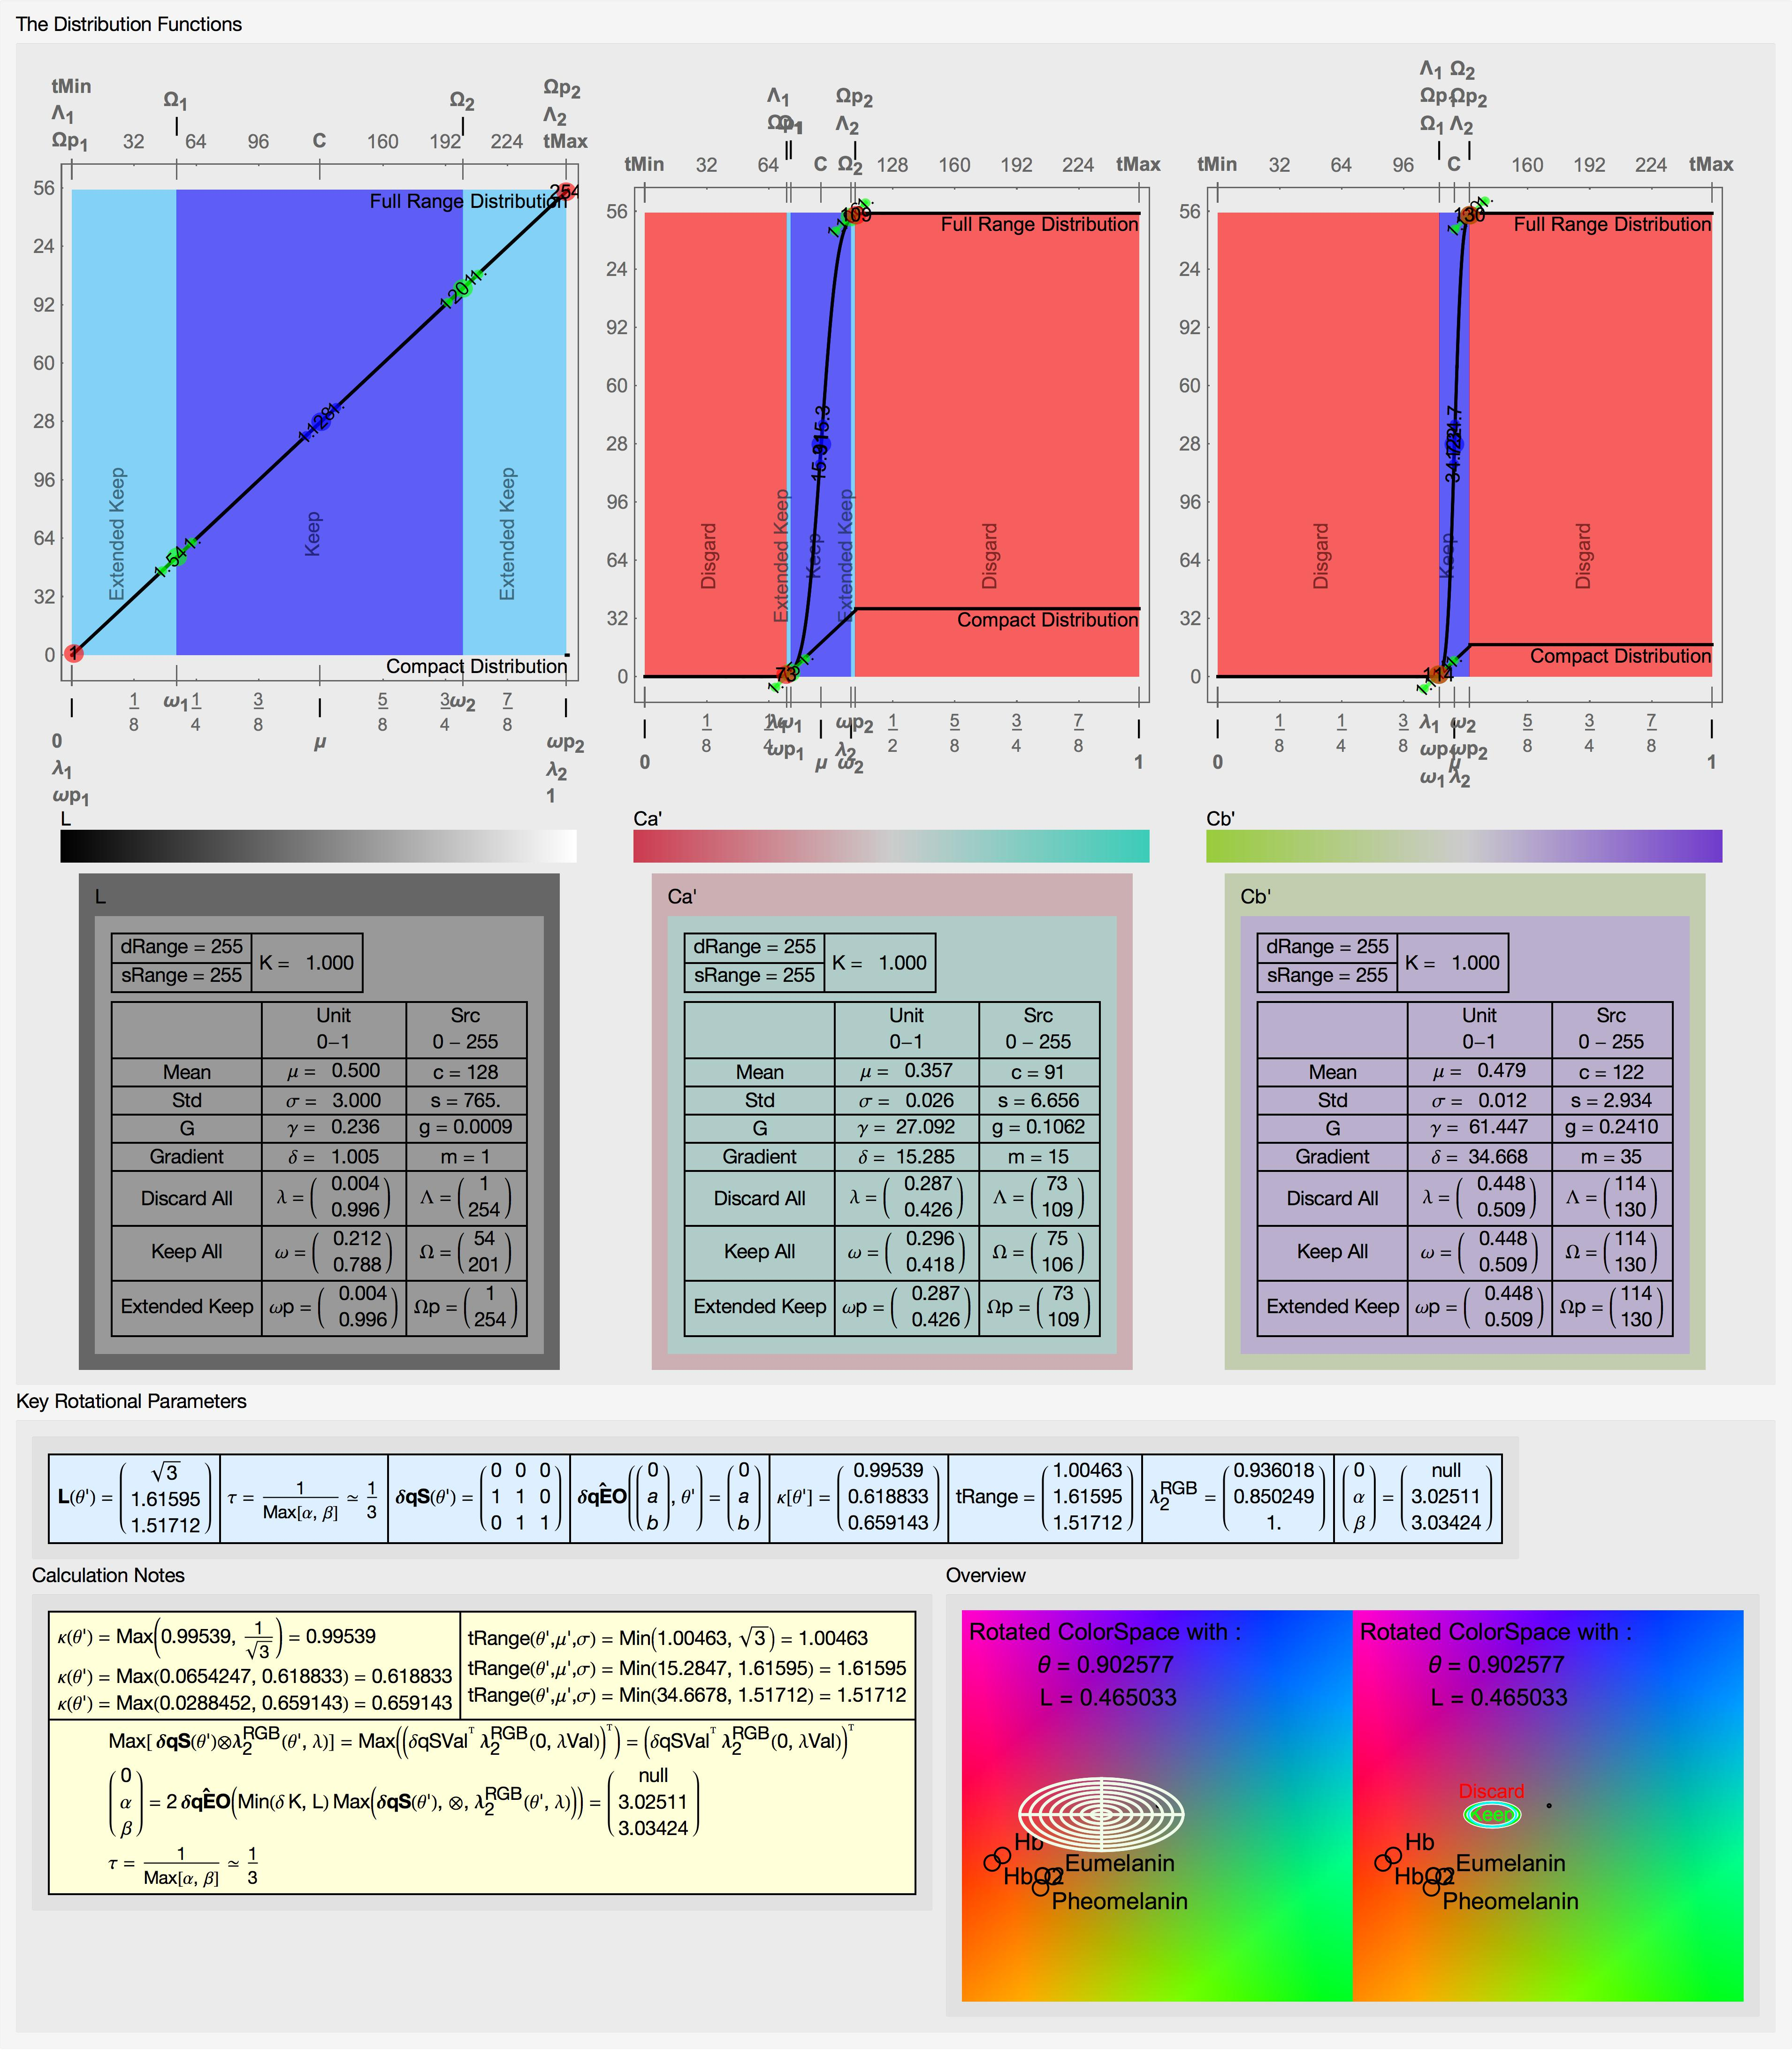
\includegraphics[width=1.0 \textwidth]{Chapter3/Figs/Distribution_Results_Final.jpg} 
    \caption{ \textbf{The Tight MATLAB fit in LCa'Cb'.} The redistribution functions for each axis alongside summary tables of the key parameters and a selection of calculations and an overview of the distribution in the new color-space.}  \label{fig:DistributionResultsFinal}
\end{figure}

It can be seen that the least square fit is a good predictor for the distribution, but the aim of the color-space is to capture all skin-relevant chromatic information. For this reason,  as well as the desire to be inclusive of skin tones outside of the sample set of three individuals, a region larger than the $2\sigma$ ellipse region (Figure \ref{fig:DistributionResultsFinal}) which is kept by the tight MATLAB fit may be desirable to be included. The $3\sigma$ ellipse region would include everything in the combined individual F,J\&N histogram. A $5\sigma$ ellipse region would  likely account for a wide variety of skin tones. 

\begin{figure}[h!]
  \centering
  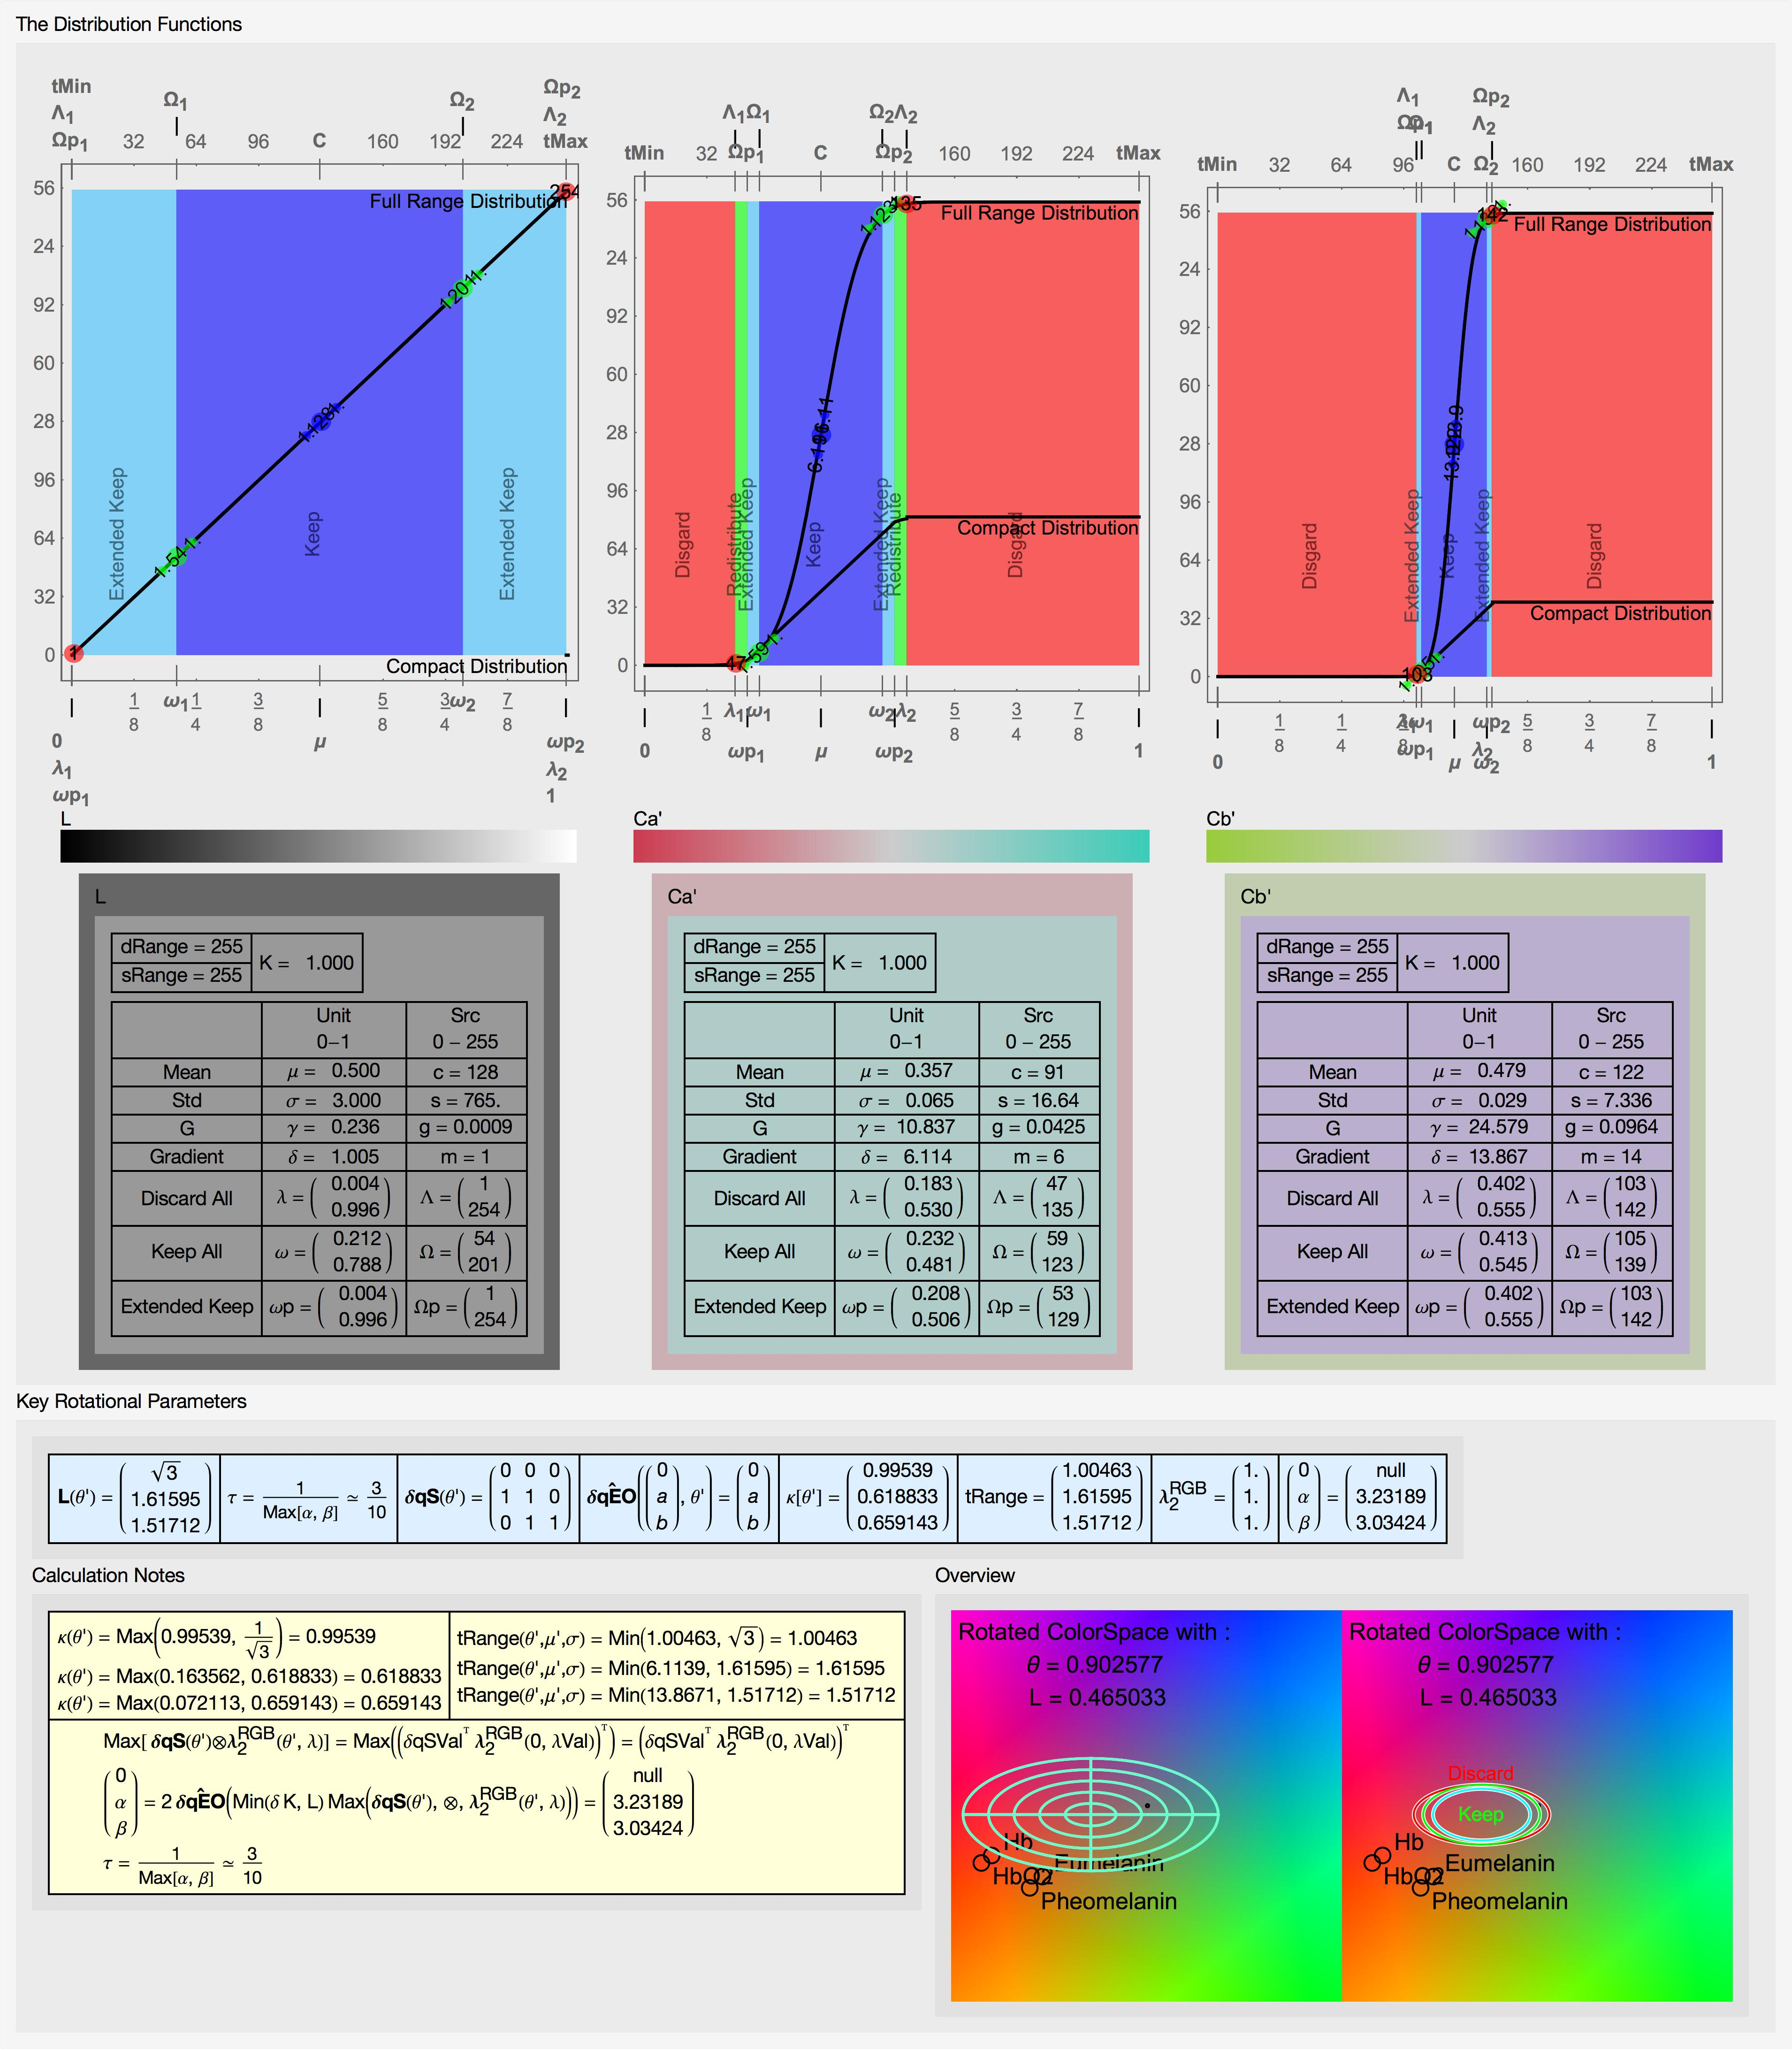
\includegraphics[width=1.0 \textwidth]{Chapter3/Figs/Distribution_Results_Final_Extended.jpg} 
    \caption{ \textbf{The extended $5\sigma$ ellipse region MATLAB fit in LCa'Cb'.} The redistribution functions for each axis alongside summary tables of the key parameters and a selection of calculations and an overview of the distribution in the new color-space. }  \label{fig:DistributionResultsFinalExtended}
\end{figure}

\begin{figure}[h!]
  \centering
  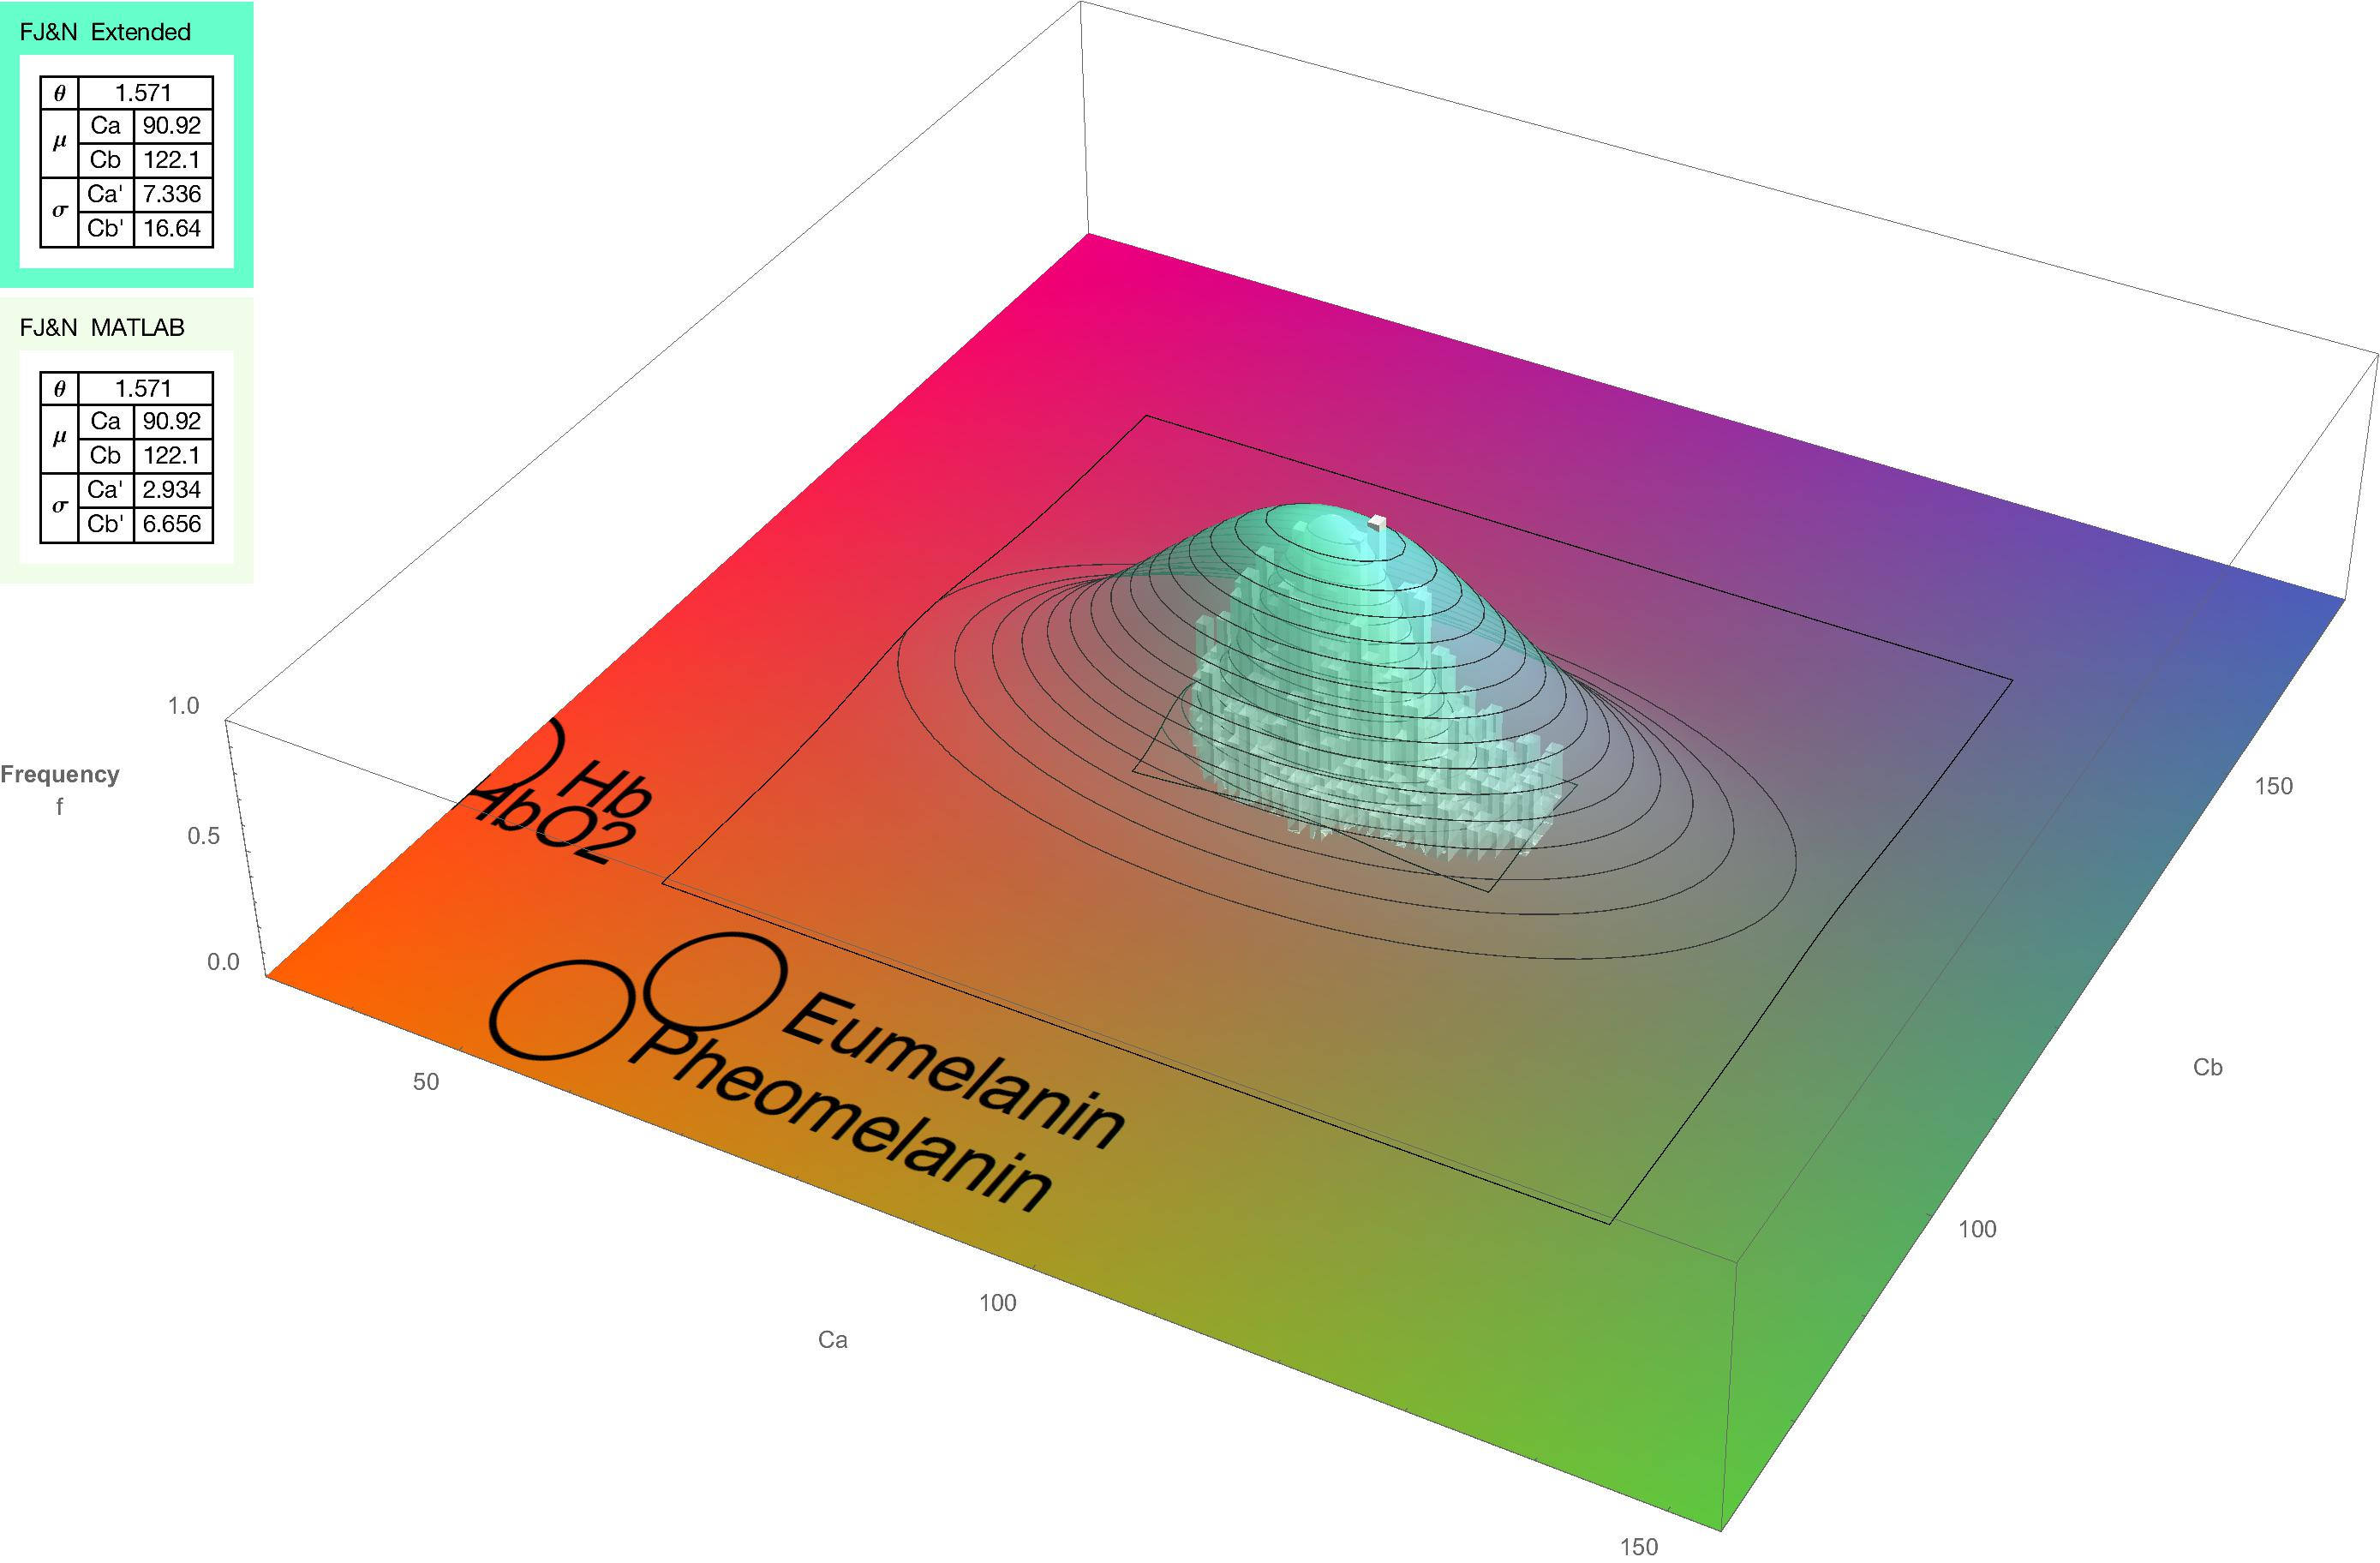
\includegraphics[width=0.95 \textwidth]{Chapter3/Figs/Distribution_Results_Final_Extended_3D.jpg} 
    \caption{ The tight and extended fits in the LCa'Cb' color-space.}  \label{fig:DistributionResultsFinalExtended3D}
\end{figure}

Extending the distribution may also affect the accuracy required in the rotation as mentioned previously. Extending out to a $5\sigma$ ellipse region does indeed affect the tolerance (Figure \ref{fig:DistributionResultsFinalExtended}), but the chosen angle perturbation $\pm0.144$ still satisfies the tolerance $\tau = 0.3094$ as $0.1441 < 0.3094$. It's also notable that the tight MATLAB distribution requires a partition in the chromatic axis while the extended distribution requires a small amount of redistribution. The tight MATLAB distribution and the extended distribution can be seen in Figure \ref{fig:DistributionResultsFinalExtended3D}.

\subsection{Conclusion}

Our goal was to find appropriate values for the 2D chromatic Gaussians in order to facilitate the image processing, and to create a color-space that preserves all of the chromatic skin information. To show that we have achieved this, we will quickly demonstrate the skin probability map:

After redistribution we have two new spaces in which to express the stats parameters: the 0:dstMax range and the new 0:1 range, where 0 and 1 correspond to different positions in the original unit space because of the compression of the information. The mean values are at the halfway point in both $c_d=dstMax/2$ and $\mu_d = \frac{1}{2}$.  The standard deviations are scaled to fit the region which is 'kept' $\sigma_d=\frac{\sigma}{\lambda_2-\lambda_1}$. The probability of a pixel in the redistributed color-space can then be found using 
\begin{equation}
P(L,Ca,Cb) = Exp(- \frac{Ca-\mu_d^{Ca} }{2 \sigma_d^{Ca}} - \frac{Cb-\mu_d^{Cb} }{2 \sigma_d^{Cb}})
\end{equation}
the result can be seen in Figure \ref{fig:TransformImages}.
\begin{figure}[h!]
  \centering
  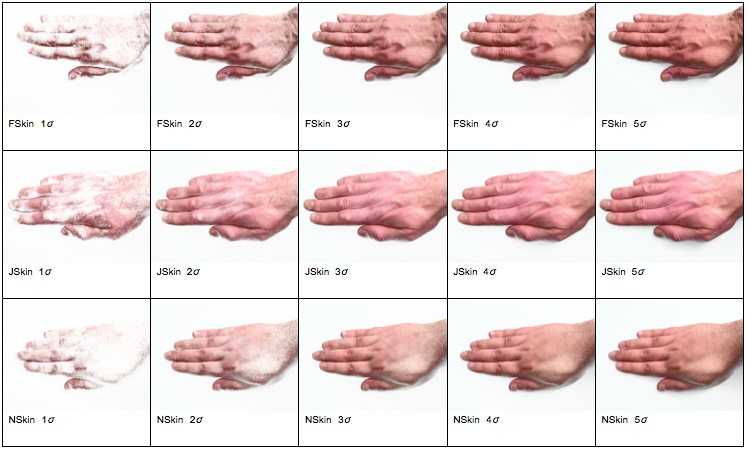
\includegraphics[width=0.95 \textwidth]{Chapter3/Figs/TransformImages.jpg} 
    \caption{ Images of hands from the three individual sets processed with the opacity given by the probability that the pixel value is skin using the simply product of Gaussians method given above.}  \label{fig:TransformImages}
\end{figure}

The probability in these images is indicated by the opacity; as can be seen, all of the skin detail is preserved, therefore all the skin information is preserved. In a normal color-space, the preservation of skin information is computationally intensive, but in the case of our bespoke color-space, it is simply the product of two 1D Gaussians, therefore finding the skin probability is a very simple function. Thus, we have preserved the skin information whilst simplifying a computer vision task. 

It should be noted that the strict $1\sigma$ result misses some of the skin; this was expected as some histogram values lie outside the Gaussian fit, so loosening the criteria is necessary to capture all of the skin information. A $2\sigma$ or $3\sigma$ criteria should be sufficient to capture all of the skin information. Additionally, the simple implementation here does not account for unreliable white-out and black-out values, or use nearest pixel values, but this is not the final step of the algorithm. For this, we need a classifier, which will be explored in the following chapter.
